\thispagestyle{empty}
\addcontentsline{toc}{section}{Segunda Etapa}

\vspace*{\fill}
\begin{center}
	{\Huge\bfseries EXAMEN GENERAL }\\[10pt]
	{\Huge\bfseries 2024-I}\\[10pt]
	{\Large\bfseries Segunda Etapa}
\end{center}
\vspace*{\fill}

\clearpage

\section*{Área: Ingenierías}

\addcontentsline{toc}{subsection}{Área: Ingenierías}


\subsection*{Aritmética}
\begin{enumerate}
	
	\item De las siguientes proposiciones, ¿Cuáles son equivalentes entre sí?
	
	I. Es necesario que Juan no vaya al cine para que termine su tarea. \\
	II. No es cierto que Juan termine su tarea y vaya al cine.\\ 
	III. Juan no termina su tarea y no va al cine.\\
	
	\begin{enumerate}[label=\alph*)]
		\item I y II
		\item I,II y III
		\item II y III
		\item I y III
		\item No son equivalentes entre sí
	\end{enumerate}
	\textbf{Respuesta correcta:} a)
	
	\vspace{2mm}
	\textbf{Solucionario:}\\[1mm]
	Sean las proposiciones\\
	p= Juan va al cine\\
	q= Juan termina su tarea\\
	
	\vspace{1mm}
	
	\textbf{Simbología:}
	
	\noindent \textbullet \quad Es necesario que Juan no vaya al cine para que termine su tarea equivale a decir: 
	\vspace{0.2cm}
	
	
	
	\begin{enumerate}[label=\Roman*.] % Configura la numeración a I., II., III.
		\item \quad $\underbrace{q}_{\text{Si Juan termina su tarea,}} \to \underbrace{\neg p}_{\text{entonces Juan no va al cine}}$
		\quad $\equiv$ \quad $\underbrace{\neg q}_{\text{Juan no termina su tarea}} \lor \underbrace{\neg p}_{\text{o no va al cine}}$\\
		\item \quad $\underbrace{\neg}_{\text{No es cierto que , }} \underbrace{(q \land p)}_{\text{Juan termine su tarea y vaya al cine}}$
		\quad $\equiv$ \quad $\underbrace{\neg q}_{\text{}} \lor \underbrace{\neg p}_{\text{}}$\\
		\item \quad $\underbrace{\neg q}_{\text{Juan no termina su tarea}} \land \underbrace{\neg p}_{\text{y no va al cine}}$\\
	\end{enumerate}
	
	\vspace{0.5cm}
	
	\noindent Son equivalentes I y II
	
	\noindent $\neg p \lor \neg q \equiv \neg (p \land q)$
	\vspace{6mm}
	
	\item En un barco habían 180 personas, ocurre un naufragio y, de los sobrevivientes, $\dfrac{2}{5}$ fuman, $\dfrac{3}{7}$ son casados y $\dfrac{2}{3}$ son ingenieros. ¿Cuántas personas sobrevivieron en dicho accidente?
	
	\begin{enumerate}[label=\alph*)]
		\item 75
		\item 105
		\item 65
		\item 95
		\item 100
	\end{enumerate}
	\textbf{Respuesta correcta:} b)
	
	\vspace{2mm}
	\textbf{Solucionario:}\\[1mm]
	
	\noindent $S + H = 180$
	
	\vspace{0.5cm}
	
	
	
	\begin{tikzpicture}[font=\normalsize]
		
		\node (S) at (4,0) {$S = \mathring{105}$};
		
		\node (F) at (0, 1.5) {$\text{Fuman } \dfrac{2}{5} S \implies S=\mathring{5}$};
		\node (C) at (0, 0) {$\text{Casados } \dfrac{3}{7} S \implies S=\mathring{7}$};
		\node (I) at (0, -1.5) {$\text{Ingenieros } \dfrac{2}{3} S \implies S=\mathring{3}$};
		
		\draw (S.west) -- (F.east);
		\draw (S.west) -- (C.east);
		\draw (S.west) -- (I.east);
	\end{tikzpicture}
	
	\vspace{0.5cm}
	
	\noindent Luego $S = 105, 210, 315, \dots$
	
	\vspace{0.5cm}
	
	\noindent Pero $S < 180 \Longrightarrow S=105$
	
	\vspace{0.5cm}
	
	\noindent Sobrevivieron las personas.
	
	\vspace{6mm}
	
	
	
	\item \noindent Halle un n\'umero de la forma: $N=32(a)(b)$, sabiendo que $a$ y $b$ son \\
	primos absolutos y que la suma de los divisores de $N$ es el triple \\
	de \'el.
	\begin{enumerate}[label=\alph*)]
		\item 325
		\item 672
		\item 323
		\item 422
		\item 642
	\end{enumerate}
	\textbf{Respuesta correcta:} b)
	
	\vspace{2mm}
	\textbf{Solucionario:}\\[1mm]
	\noindent Como $N = 2^5. a . b$
	
	\noindent Dato: $\text{SD}_{(N)} = 3 (N)$
	
	\noindent $\dfrac{2^{6}-1}{2-1} \cdot \dfrac{a^{2}-1}{a-1} \cdot \dfrac{b^{2}-1}{b-1} = 3 (2^5 . a.b)$
	
	\noindent $63 (a+1)(b+1)= 3_\cdot 2^5.a.b$
	
	\noindent $3_\cdot 7 (a+1)(b+1)= a.b.(4)(8) $
	
	\vspace{0.1cm}
	
	
	
	\noindent Comparando $a=3$ y $b=7$
	
	\vspace{0.1cm}
	
	\noindent Luego $N=32(3)(7)$
	
	\noindent \fbox{$N=672$}
	
	\vspace{6mm}
	
	\item Si $N$ se eleva al cuadrado y se le resta la unidad, es divisible entre 8, además el \text{MCM} de $N$ y el cociente obtenido es $3720$. Halle dicho cociente.
	\begin{enumerate}[label=\alph*)]
		\item 110
		\item 98
		\item 108
		\item 112
		\item 120
	\end{enumerate}
	\textbf{Respuesta correcta:} e)
	
	\vspace{2mm}
	\textbf{Solucionario:}
	
	\begin{flalign*}
		&\quad N^2 - 1 = \mathring{8} \text{ donde } q = \dfrac{N^2 - 1}{8} & \\
		&\quad \text{MCM}(N, q) = 3720 & \\
		&\quad \text{MCM} \underbrace{\left(N, \dfrac{N^2 - 1}{8}\right)}_{\text{PESI}} =\dfrac{N(N^2 - 1)}{8} = 3720 & \\
		&\quad \implies N(N^2 - 1) = 8(3720) \implies N = 31 & \\
		&\quad \therefore q = \dfrac{31^2 - 1}{8} =\fbox{120} &
	\end{flalign*}
	
	\vspace{6mm}
	
	
	
\end{enumerate}


\subsection*{Álgebra}

\begin{enumerate}[resume]
	
	\item  \text{Si el rango de la función } y = $\dfrac{4x}{x^2+1}$ \text{ es el intervalo } [a, b], \text{ calcule } $a^2 + b^2$.
	
	\begin{enumerate}[label=\alph*)]
		\item 5
		\item 8
		\item 10
		\item 4
		\item 2
	\end{enumerate}
	\textbf{Respuesta correcta:} b)
	
	\vspace{2mm}
	\textbf{Solucionario:}
	
	
	
	\begin{flalign*}
		&\quad \text{Dom } g(x) = \mathbb{R}; \quad y = \dfrac{4x}{x^2+1} & \\
		&\quad yx^2 - 4x + y = 0 & \\
		&\quad \Delta = (-4)^2 - 4yy \ge 0 & \\
		&\quad 16 \ge 4y^2 \implies 4 \ge y^2 & \\
		&\quad -2 \le y \le 2 \quad y \in [-2, 2] & \\
		&\quad a^2 + b^2 = 4 + 4 =\fbox{ 8 }&
	\end{flalign*}
	
	\vspace{6mm}
	
	\item Sean los polinomios idénticos:
	\begin{flushleft}
		
		$P(x) = 2x^{3} + 5x^{2} + 4x + 1$
		
		
		$Q(x) = (ax + b)^{c}\,(cx + d)^{a} + K, \qquad K \ne 1$
		
		\text{Calcule } 
		
		$\left( \dfrac{b^{\,c}\, d^{\,a}}{1 - K} \right)(a^{\,c} c^{\,a})$
		
	\end{flushleft}
	
	
	
	
	\begin{enumerate}[label=\alph*)]
		\item -1
		\item 2
		\item 1
		\item -2
		\item 4
	\end{enumerate}
	\textbf{Respuesta correcta:} b)
	
	\vspace{2mm}
	\textbf{Solucionario:}
	
	Los términos independientes son iguales $1 = b^c d^a + k $ $\Longrightarrow$   $1-k = b^c d^a$ \\
	
	Coeficiente principal igual:
	$2 = a^c.c^a$
	
	$\therefore \left(\dfrac{b^d c^a}{(1-k)}\right) (a^c.c^a) = \left(\dfrac{1-k}{1-k}\right) (2) =$\fbox{$ 2$}
	
	\vspace{6mm}
	
	\item Resuelva la siguiente ecuasion:\\
	$$\log_x(5-x) + \dfrac{1}{\log_{(x+2)} x} = \log_x 6$$
	\text{Y calcule el valor de } $\log_{64} x^2$
	
	\begin{enumerate}[label=\alph*)]
		\item 0
		\item $\dfrac{2}{3}$
		\item $\dfrac{1}{2}$
		\item $\dfrac{1}{4}$
		\item $\dfrac{1}{3}$
	\end{enumerate}
	\textbf{Respuesta correcta:} b)
	
	\vspace{2mm}
	\textbf{Solucionario:}
	
	
	\begin{align*}
		\log_x (5-x) + \dfrac{1}{\log_{(x+2)} x} &= \log_x 6 \\
		&= \log_x (5-x) + \log_x (x+2) \\
		&= \log_x [(5-x)(x+2)] \\
		&= \log_x (10 + 3x - x^2) \\
		&= \log_x 6 \\
		\therefore 10 + 3x - x^2 &= 6 \\
		\implies x^2 - 3x - 4 &= 0 \\
		(x-4)(x+1) &= 0
	\end{align*}
	\text{de donde } x=4 \quad \text{ó } x=-1
	\text{tomemos } x=4
	\begin{align*}
		\log_{64} x^2 &= \log_{64} 4^2 \\
		&= \log_{2^6} 2^4 \\
		&= \dfrac{4}{6} \\
		&= \fbox{$\dfrac{2}{3}$}
	\end{align*}
	
	\vspace{6mm}
	
	\item \text{Dada la matriz }$ A = (a_{ij})_{3\times3}$ \text{ definida por:}
	\[
	a_{ij} =
	\begin{cases}
		3 - a_{ij}, & \text{si } i \neq j,\\[4pt]
		-a_{ij},    & \text{si } i = j.
	\end{cases}
	\]
	
	\text{Calcule } $|A|$
	
	
	\begin{enumerate}[label=\alph*)]
		\item 0
		\item 1
		\item $\dfrac{2}{7}$
		\item $\dfrac{27}{4}$
		\item $\dfrac{9}{4}$
	\end{enumerate}
	\textbf{Respuesta correcta:} d)
	
	\vspace{2mm}
	\textbf{Solucionario:}
	
	\[
	a_{ij} =
	\begin{cases}
		3 - a_{ij}, & \text{si } i \neq j,\\[6pt]
		-a_{ij},    & \text{si } i = j.
	\end{cases}
	\qquad\Rightarrow\qquad 
	\begin{aligned}
		a_{11} = -a_{11} &\Rightarrow a_{11} = 0 \\[6pt]
		a_{12} = 3 - a_{12} &\Rightarrow a_{12} = \dfrac{3}{2} \\[6pt]
		a_{13} = 3 - a_{13} &\Rightarrow a_{13} = \dfrac{3}{2} \\[6pt]
		a_{21} = 3 - a_{21} &\Rightarrow a_{21} = \dfrac{3}{2}
	\end{aligned}
	\]
	
	\[
	\text{Luego, } 
	A = 
	\begin{pmatrix}
		0 & 3/2 & 3/2 \\
		3/2 & 0 & 3/2 \\
		3/2 & 3/2 & 0
	\end{pmatrix}
	\qquad\Rightarrow\qquad 	
	A = \dfrac{3}{2}
	\begin{pmatrix}
		0 & 1 & 1 \\
		1 & 0 & 1 \\
		1 & 1 & 0
	\end{pmatrix}
	\]
	
	
	$|A|= \left(\dfrac{3}{2}\right)^3 \bigl(0 + 1 + 1 - 0 - 0 - 0\bigr)$
	
	
	
	$|A| = \dfrac{27}{8}(2)=$\fbox{$ \dfrac{27}{4}$}
	
	
\end{enumerate}	


\subsection*{Geometría}

\begin{enumerate}[resume]
	
	\item \text{En la figura, ABCDE es un polígono Regular.}
	
	\text{Halle} |x|.
	
	\begin{center}
		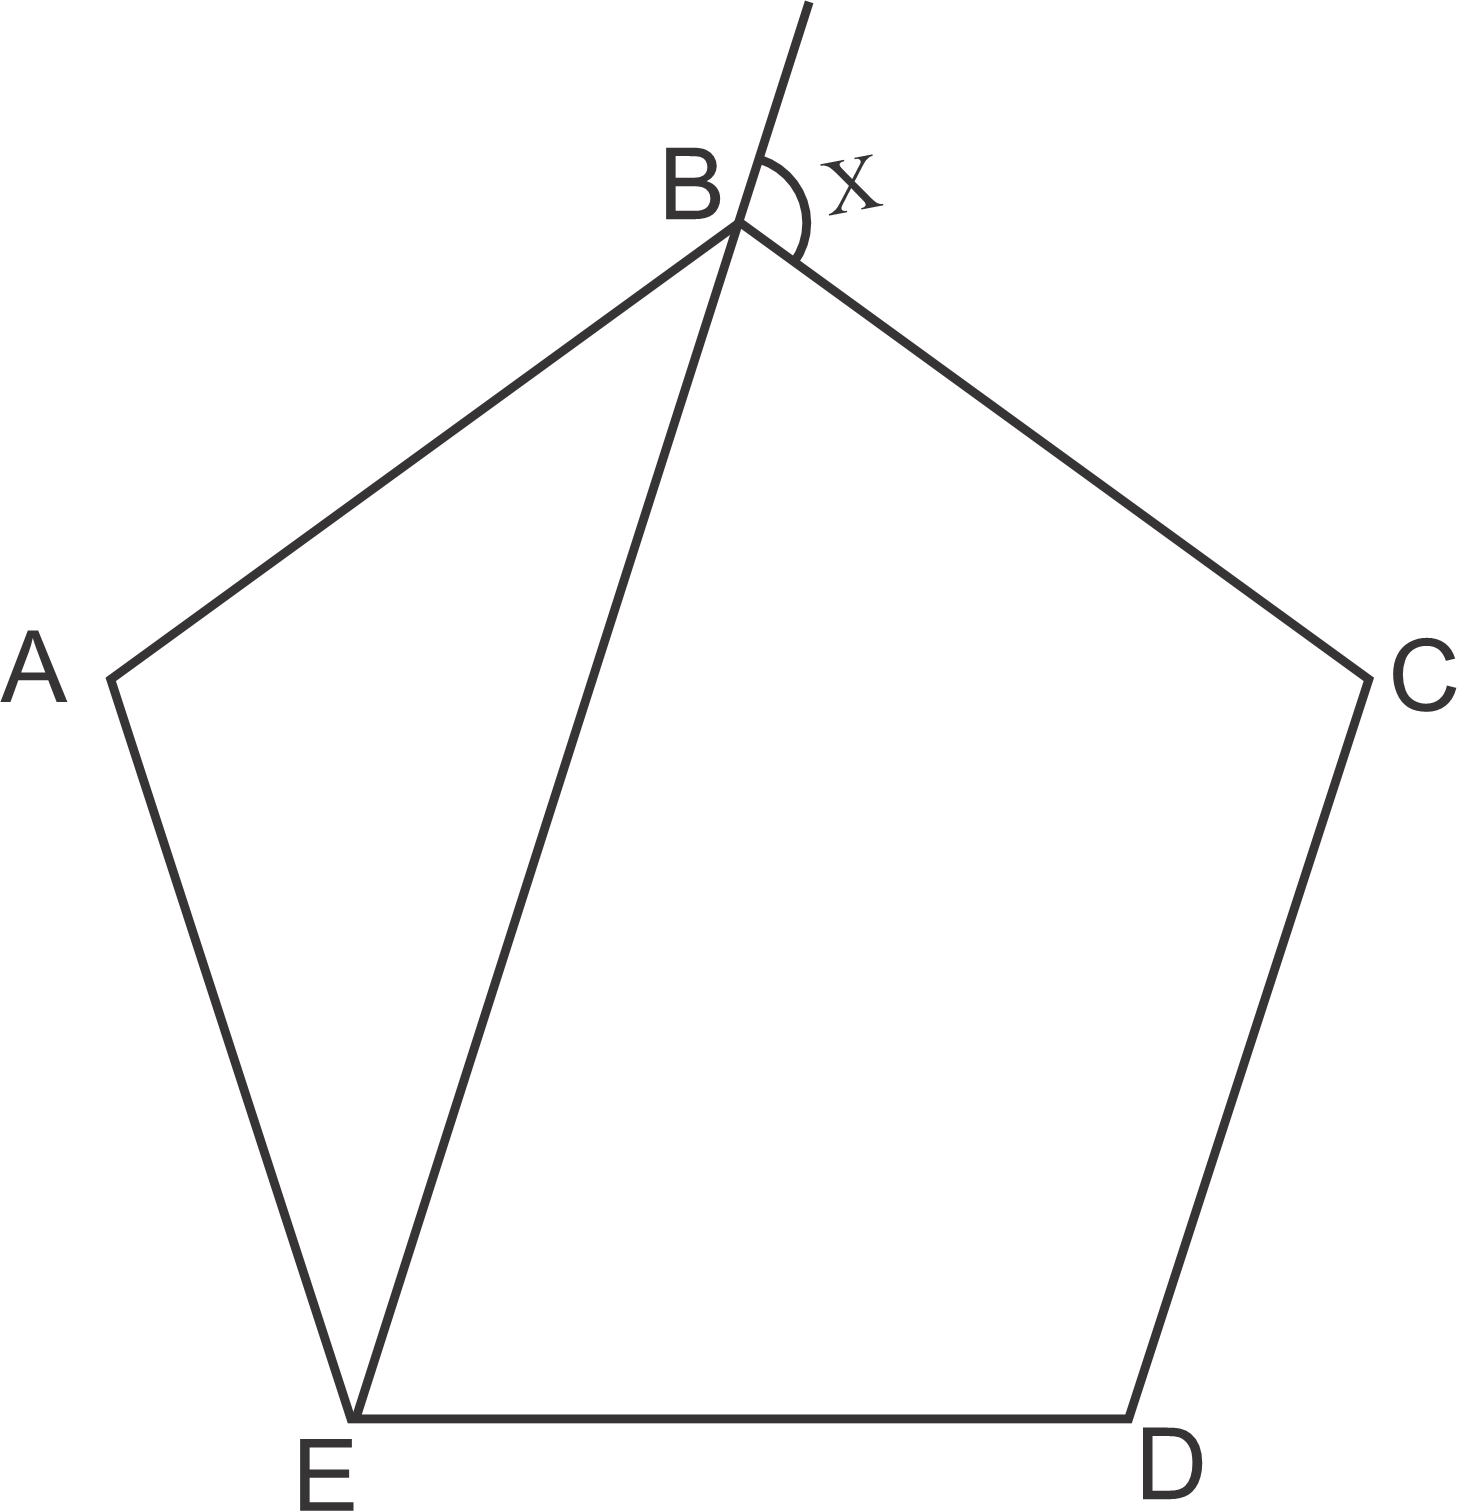
\includegraphics[width=4cm]{imagenes/general2024-I/etapa2/ing/Enunciado-1.png}\par\vspace{2cm}
	\end{center}
	\vspace{1mm}	
	\begin{enumerate}[label=\alph*)]
		\item 36°
		\item 72°
		\item 108°
		\item 120°
		\item 144°
	\end{enumerate}
	
	\textbf{Respuesta correcta:} c)
	
	\vspace{2mm}
	\textbf{Solucionario:}
	
	De la figura  se tiene
	
	$x+72^\circ=180^\circ$
	
	$x=180^\circ-72^\circ$
	
	\fbox{$x=108°$}
	
	
	\begin{center}
		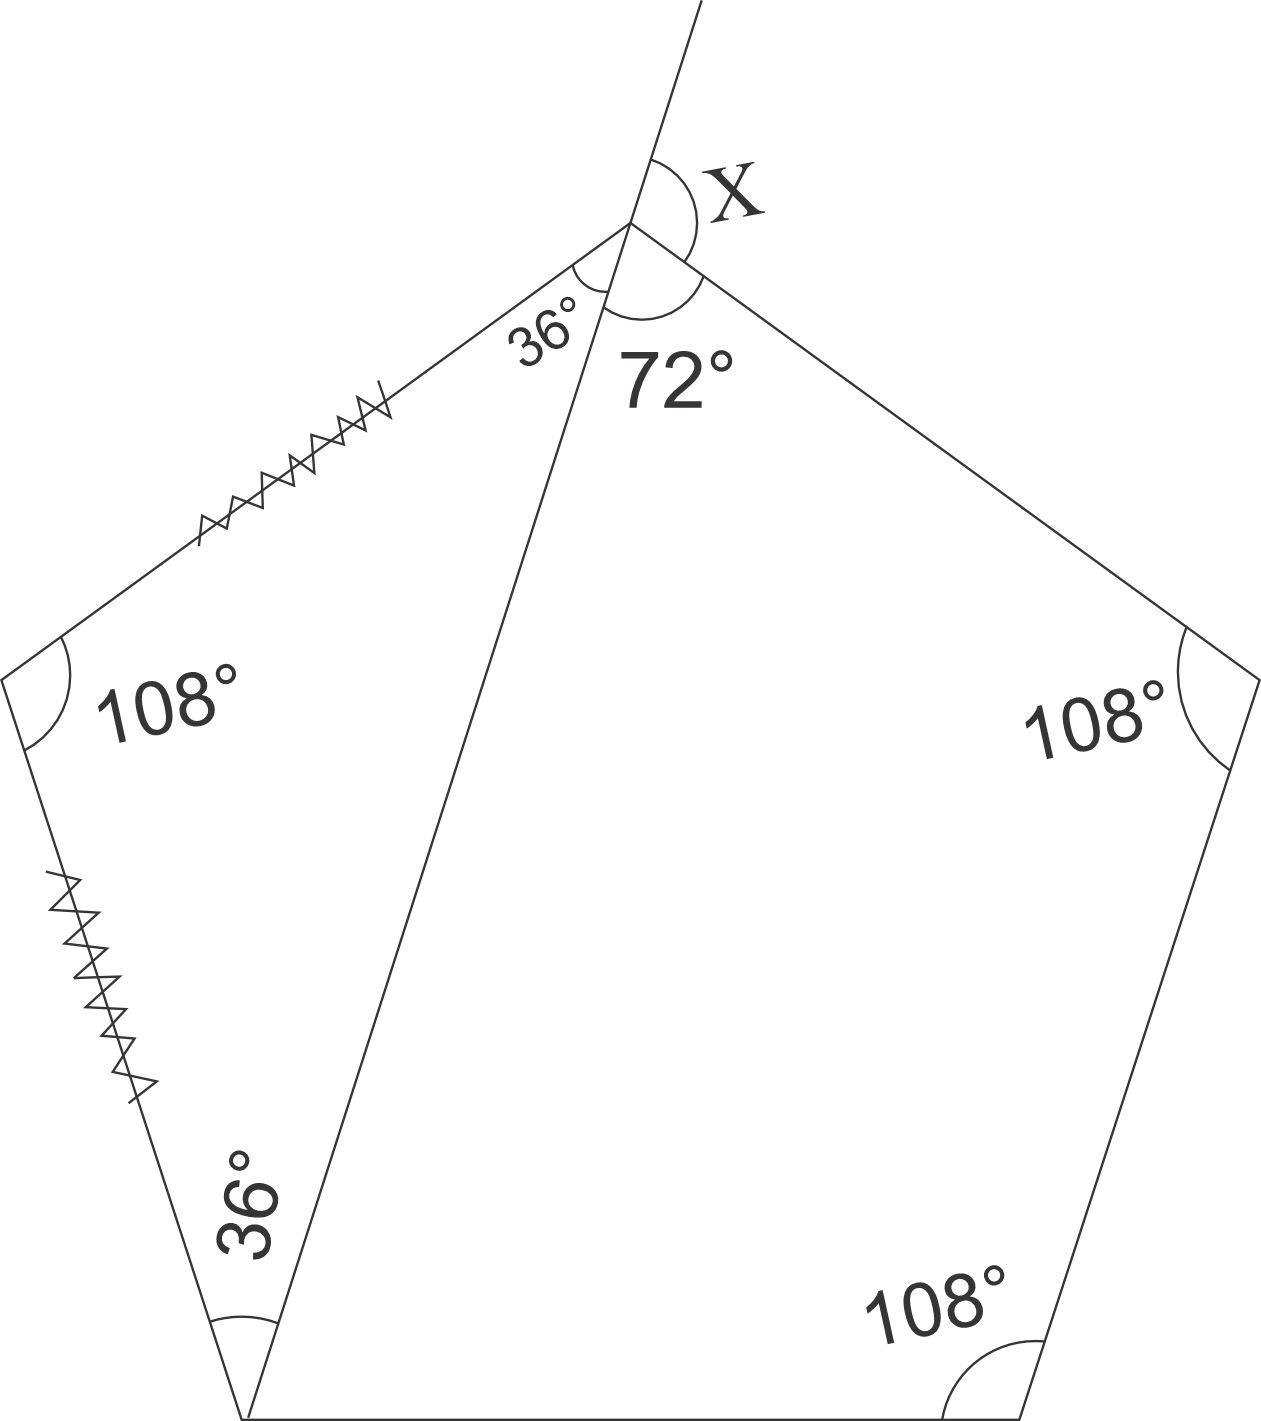
\includegraphics[width=4cm]{imagenes/general2024-I/etapa2/ing/Pgeometria1.png}\par\vspace{2cm}
	\end{center}
	
	
	\item En un cono circular recto de 9cm de altura y 15 cm de radio, se inscribe un cilindro circular recto de 5cm de radio tal que una de sus bases está sobre la base del cono. Calcule el volumen del cilindro.
	\begin{enumerate}[label=\alph*)]
		\item 120 $\pi cm^3$
		\item 130 $\pi cm^3$
		\item 140 $\pi cm^3$
		\item 150 $\pi cm^3$
		\item 160 $\pi cm^3$
	\end{enumerate}
	
	\textbf{Respuesta correcta:} d)
	
	\vspace{2mm}
	\textbf{Solucionario:}
	
	\begin{center}
		\begin{minipage}{0.45\textwidth}
			Por semejanza de triángulos:\\[0.2cm]
			$\dfrac{9-x}{9}=\dfrac{5}{15}$\\
			
			$9-x=\dfrac{9}{3}$\\
			
			$9-x=3$\\
			$x=6$\\
			$V_{cilindro}$ $= \pi r^2h$\\
			
			$=\pi (5)^2 * 6 $\\
			\fbox{$=150\pi cm^3$}
			\vspace{6mm}
		\end{minipage}
		\hfill
		\begin{minipage}{0.45\textwidth}
			\centering
			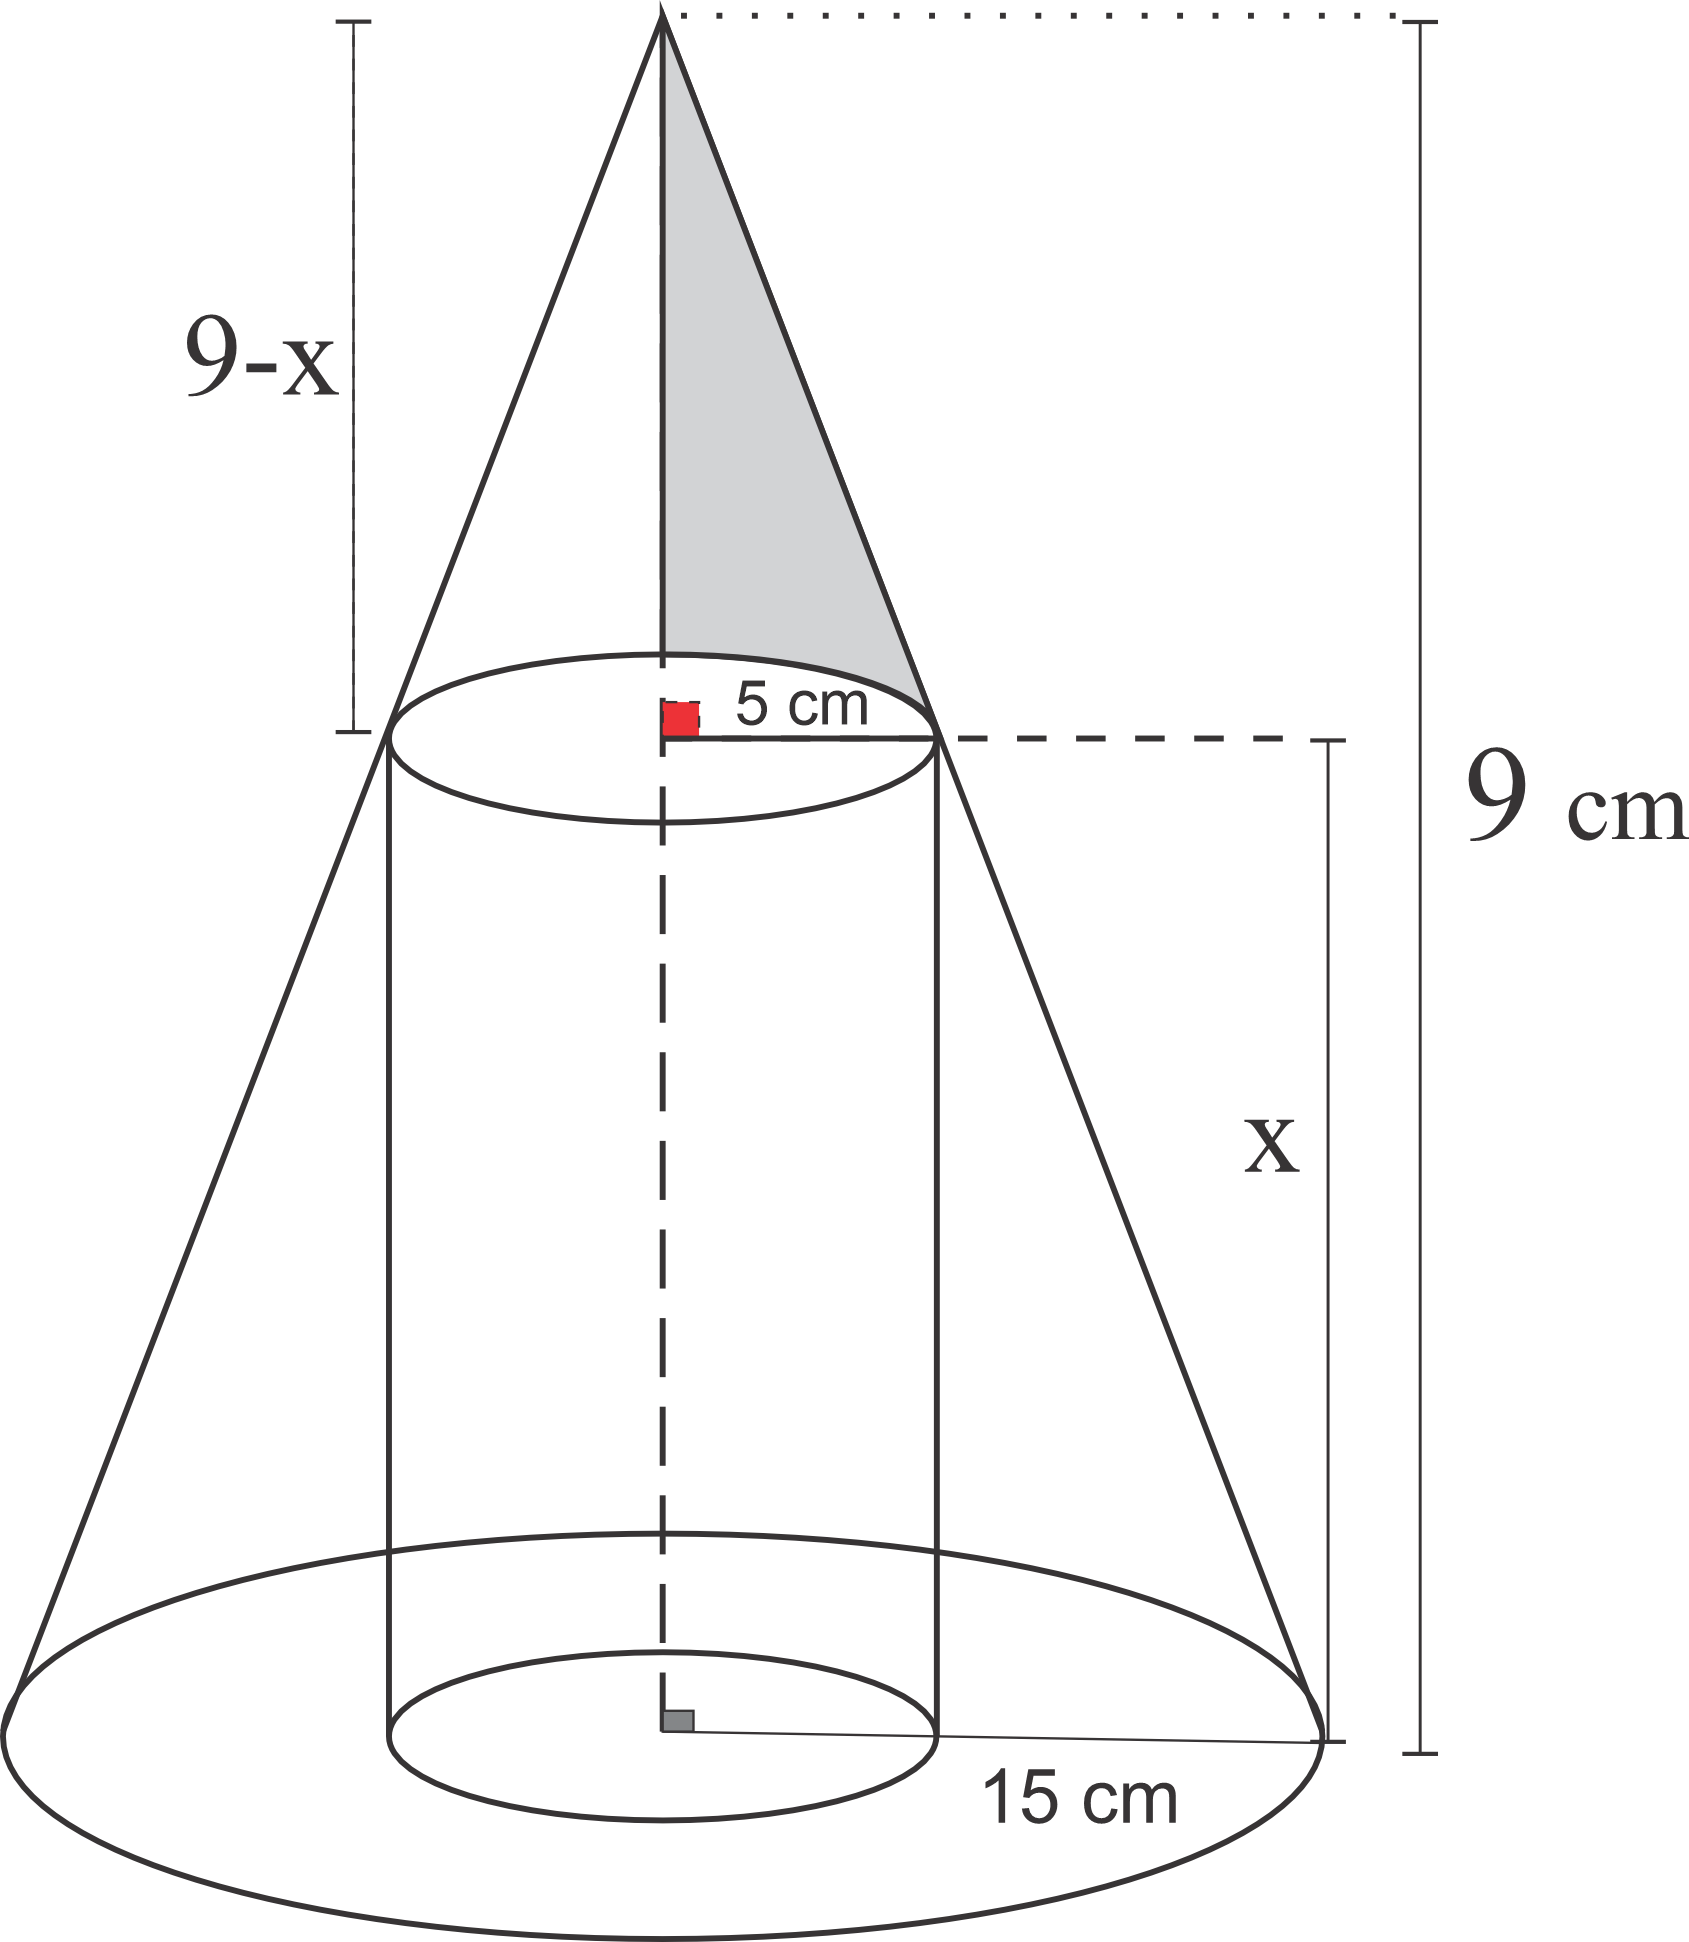
\includegraphics[width=3.5cm]{imagenes/general2024-I/etapa2/ing/problema-2.png}
		\end{minipage}
	\end{center}
	
	
	
	\item Un depósito de agua en la UNA-PUNO tiene sección transversal parabólica. Cuando el nivel del agua alcanza una altura de 18m, su ancho mide 24m.halle el ancho del nivel del agua cuando este desciende 10m. 
	\begin{enumerate}[label=\alph*)]
		\item 8 m
		\item 16 m
		\item 32 m
		\item 25 m
		\item 20 m
	\end{enumerate}
	
	\textbf{Respuesta correcta:} b)
	
	\vspace{2mm}
	\textbf{Solucionario:}

	\begin{center}
		\begin{minipage}{0.45\textwidth}
			De la fig:\\
			$\mathscr{P} : x^2=4py$
			
			$\bullet  12^2=4p(18) \longrightarrow p=2$\\
			
			$\bullet  a^2=4(2)(8) \longrightarrow  a=8$\\
			
			
			
			$\therefore$ El nuevo Ancho del agua $= 8+8=$\fbox{$16$	}
			\vspace{6mm}
		\end{minipage}
		\hfill
		\begin{minipage}{0.45\textwidth}
			\centering
			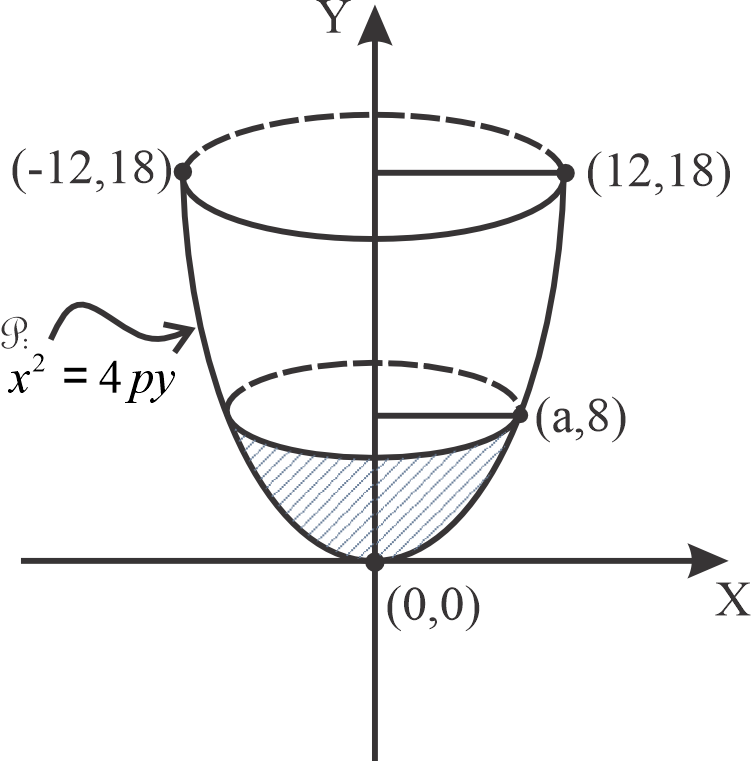
\includegraphics[width=4.3cm]{imagenes/general2024-I/etapa2/ing/problema 3 geometris.png}
		\end{minipage}
	\end{center}
	

	\vspace{6mm}
	
	\item Halle  la longitud de la figura  continua si m$\overset{\frown}{EF}
	$ es 60°y los demas arcos son semicicunferencias de igual radio.
	
	
	
	\begin{center}
		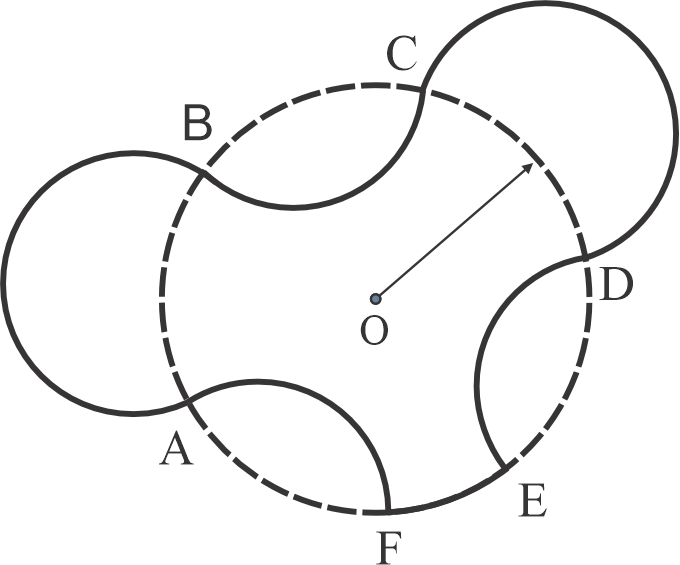
\includegraphics[width=4.3cm]{imagenes/general2024-I/etapa2/ing/probgeometria4.png}\par
		\vspace{2cm}
	\end{center}
	
	
	
	\begin{enumerate}[label=\alph*)]
		\item $\dfrac{15\pi}{2}R$
		\item $\dfrac{16\pi}{3}R$
		\item $\dfrac{17\pi}{6}R$
		\item $18\pi R$
		\item $\dfrac{19\pi}{3}R$
	\end{enumerate}
	
	\textbf{Respuesta correcta:} c)
	
	\vspace{2mm}
	\textbf{Solucionario:}
	
	$
	L_{\text{total}}
	= 5L + L_{\overset{\frown}{EF}}
	$
	
	$
	= 5(\pi r) + \dfrac{2\pi R\,\theta}{360^\circ}
	$
	
	$
	= 5\!\left(\dfrac{2\pi\left(\tfrac{R}{2}\right)}{2}\right)
	+ \dfrac{2\pi R(60^\circ)}{360^\circ}
	$
	
	$
	= \dfrac{5\pi R}{2} + \dfrac{\pi R}{3}
	$
	
	\fbox{$
	= \dfrac{17\pi R}{6}
	$}
	
	
	\vspace{6mm}
\end{enumerate}


\subsection*{Trigonometría}

\begin{enumerate}[resume]
	
	\item Un niño y dos árboles se encuentran en una misma línea. El niño que está entre los árboles observa las partes superiores de dichos árboles con ángulos de elevacion $\alpha$ y $2\alpha$. Si se sabe que sus respectivas visuales miden 30 y 35 metros,Calcule la altura del mayor árbol, temiendo en cuenta que la distancia a la que encuentra el niño de un árbol es igual a la altura del otro árbol y ese último es el que se opone a $2\alpha$.
	\begin{enumerate}[label=\alph*)]
		\item $\dfrac{60}{7}m$
		\item $\dfrac{40}{7}m$
		\item $\dfrac{60\sqrt{10}}{7}m$
		\item $\dfrac{50\sqrt{10}}{7}m$
		\item $\dfrac{45\sqrt{10}}{7}m$
	\end{enumerate}
	
	\textbf{Respuesta correcta:} b)
	
	\vspace{2mm}
	\textbf{Solucionario:}
	
	
	\begin{center}
		\begin{minipage}{0.45\textwidth}
			Igualando\\
			$35\sen2 \alpha =30\cos \alpha$\\
			
			$35(2\sen \alpha \cos\alpha)=30\cos\alpha$\\
			
			$\sen \alpha=\dfrac{3}{7}$\\
			
			$x=30$.$\cos\alpha$\\
			
			$x=30$.$\dfrac{2\sqrt{10}}{7}=$\fbox{$\dfrac{60\sqrt{10}}{7} $}
			\vspace{6mm}
		\end{minipage}
		\hfill
		\begin{minipage}{0.45\textwidth}
			\centering
			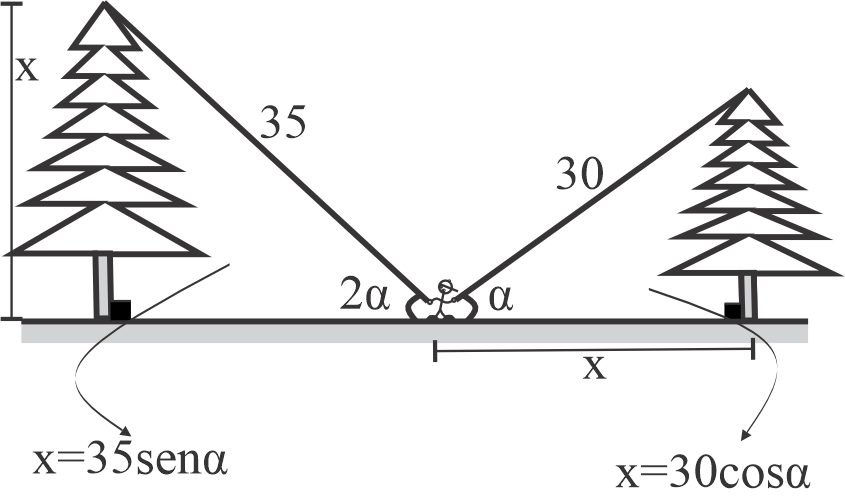
\includegraphics[width=4.5cm]{imagenes/general2024-I/etapa2/ing/trigonometria-1.png}
		\end{minipage}
	\end{center}
	
	
	
	\vspace{6mm}
	
	\item En la figula mostrada, determine $\tan$ $\theta$
	\begin{center}
		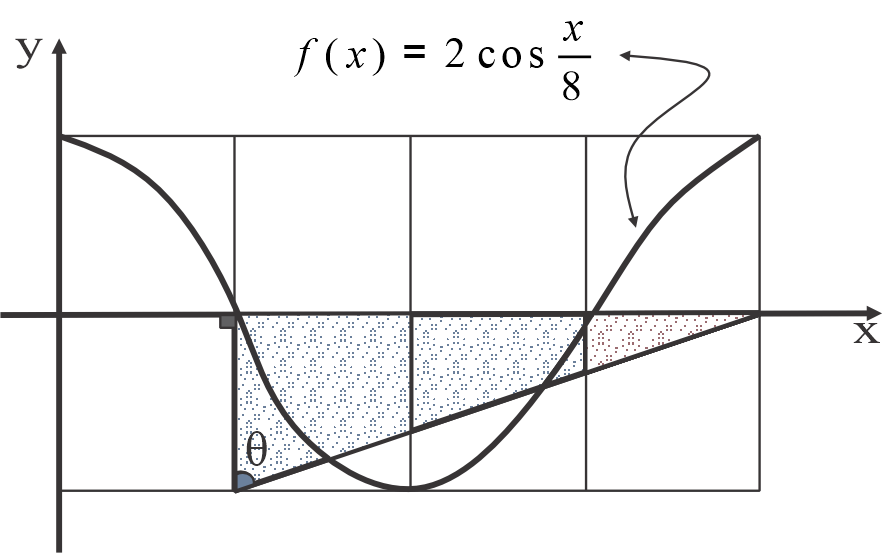
\includegraphics[width=4.8cm]{imagenes/general2024-I/etapa2/ing/trigonometria-2.png}
	\end{center}
	
	\begin{enumerate}[label=\alph*)]
		\item 5$\pi$
		\item 2$\pi$
		\item 4$\pi$
		\item 6$\pi$
		\item 3$\pi$
	\end{enumerate}
	
	\textbf{Respuesta correcta:} d)
	
	\vspace{2mm}
	\textbf{Solucionario:}
	
	\begin{center}
		\begin{minipage}{0.45\textwidth}
			$ \bigstar w=\dfrac{1}{8}$\\
			
			$\dfrac{2\pi}{T}=\dfrac{1}{8}$\\
			
			$T=16\pi $\\
			
			$\bigstar A=2$\\
			
			$\tan \theta =\dfrac{12\pi}{2}=$\fbox{$6\pi$}
			
			\vspace{6mm}
		\end{minipage}
		\hfill
		\begin{minipage}{0.45\textwidth}
			\centering
			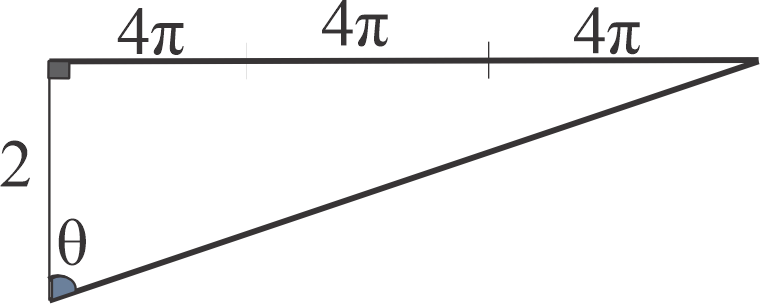
\includegraphics[width=4.5cm]{imagenes/general2024-I/etapa2/ing/trigonometria-2.2.png}
		\end{minipage}
	\end{center}

\item En el gráfico,calcular el valor de:

$M=12\cos\theta - 5 \cos\alpha.$
\begin{center}
	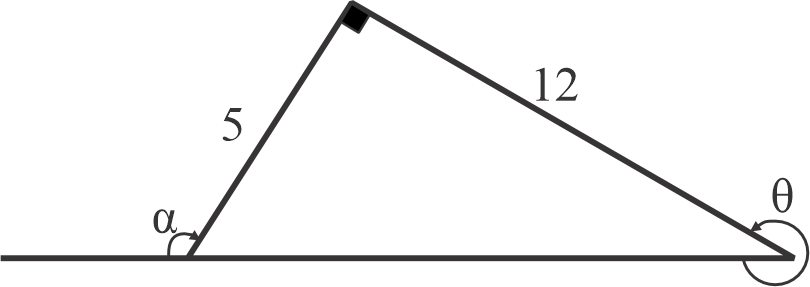
\includegraphics[width=4.5cm]{imagenes/general2024-I/etapa2/ing/trigonometria-3.png}
\end{center}


\begin{enumerate}[label=\alph*)]
	\item 26
	\item 15
	\item 11
	\item 14
	\item 13
\end{enumerate}

\textbf{Respuesta correcta:} e)

\vspace{2mm}
\textbf{Solucionario:}

	\begin{center}
	\begin{minipage}{0.45\textwidth}
		$\cos(\overbrace{360°-\theta}^{\text{$IV_c$}})=\cos\theta=\dfrac{12}{13}$\\
		$\cos(\overbrace{180°-\alpha}^{\text{$II_c$}})=-\cos\alpha=\dfrac{5}{13}$\\
		Reemplazando: \\
		$M= 12 \cos\theta-5\cos\alpha$\\
		
		$M=12(\dfrac{12}{13})-5(\dfrac{-5}{13})$\\
		
		$M=\dfrac{144+25}{13}=\dfrac{13^2}{13}=$\fbox{$13$}
		\vspace{5mm}
	\end{minipage}
	\hfill
	\begin{minipage}{0.45\textwidth}
		\centering
		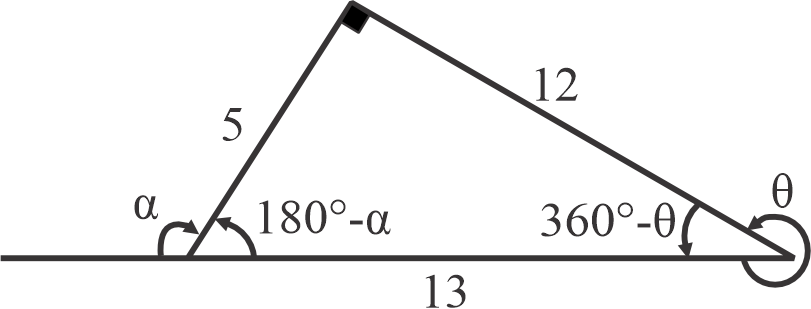
\includegraphics[width=4.5cm]{imagenes/general2024-I/etapa2/ing/trigonometria-3.3.png}
	\end{minipage}
\end{center}


\vspace{6mm}

		

	\item Determine la Variación de:\\
	
	$K= \dfrac{\sen\alpha-2}{\sen\alpha+2},\alpha \in  III_c$\\
	
\begin{enumerate}[label=\alph*)]
	\item $\langle-2;0\rangle$
	\item $\langle-3;-1\rangle$
	\item $\langle-4;-2\rangle$
	\item $\langle-3;0\rangle$
	\item $\langle-2;-1\rangle$
\end{enumerate}
\textbf{Respuesta correcta:} c)

\vspace{2mm}
\textbf{Solucionario:}

$K= \dfrac{\sen\alpha+2}{\sen\alpha+2}-\dfrac{4}{\sen\alpha+2}$

$K= 1-\dfrac{4}{\sen\alpha+2}$

$III_c \rightsquigarrow -1< \sen\alpha < 0  $

$1< \sen\alpha+2 < 2$

$1>\dfrac{1}{5\alpha+2}>\dfrac{1}{2}$

$-4<\dfrac{-4}{5\alpha+2}<-2 $

$-3<1-\dfrac{4}{5\alpha+2}<-1 $

$-3<K<-1 $

	\fbox{
$\langle-3;-1\rangle$
}
\vspace{6mm}

\end{enumerate}

\vspace{6mm}


\subsection*{Física}


\begin{enumerate}[resume]
	
	\item En la figura, se demuestra una esferaque tiene una carga de 10C y una masa de 5kg,que se encuentra en equilibrio mecánico dentro de un campo eléctrico uniforme de 5N/C, unida a una cuerda no conductora. Determine el ángulo $\theta$ que dorma la cuerda con el eje vertical.$(g=10 m/s_2)$
	\begin{enumerate}[label=\alph*)]
		\item 60°
		\item 45°
		\item 30°
		\item 53°
		\item 37°
	\end{enumerate}
	\textbf{Respuesta correcta:} b)
	
	\vspace{2mm}
	\textbf{Solucionario:}\\[1mm]
	
	
	
	
	\begin{center}
		\begin{minipage}{0.45\textwidth}
		$\sum F_x=0$\\
		
		$T\sen\theta=Eq..............I$	\\
		
		$\sum F_y=0 $\\
		
		$ T\cos\theta=mg..............II$\\
		
			\vspace{6mm}
		\end{minipage}
		\hfill
		\begin{minipage}{0.45\textwidth}
			\centering
			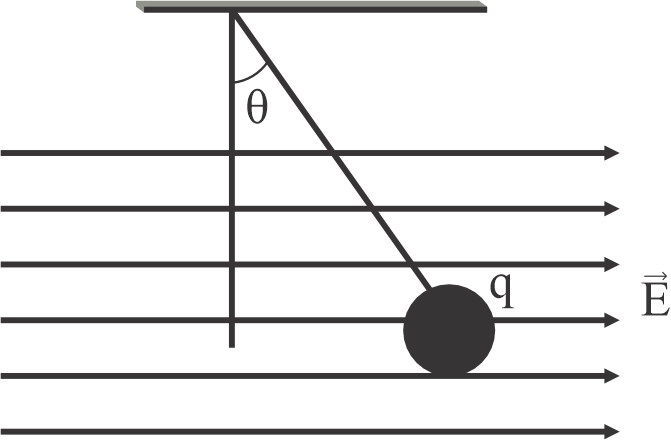
\includegraphics[width=4.5cm]{imagenes/general2024-I/etapa2/ing/fisica-1.png}
		\end{minipage}
	\end{center}
	
	
	
	\begin{center}
		\begin{minipage}{0.45\textwidth}
		$I \div II$\\
		
		$\dfrac{T\sen\theta}{T\cos\theta}=\dfrac{Eq}{mg}$\\
		
		$\tan\theta=\dfrac{(5)(10)}{(5)(10)}=1$\\
		
			\fbox{
		$\theta=45°$
	}
			\vspace{6mm}
		\end{minipage}
		\hfill
		\begin{minipage}{0.45\textwidth}
		\centering
		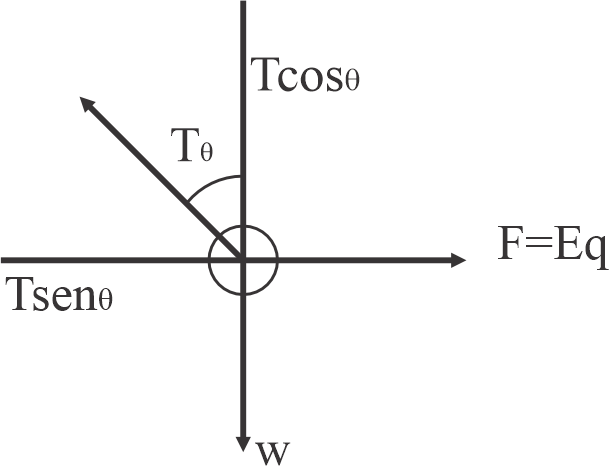
\includegraphics[width=4.5cm]{imagenes/general2024-I/etapa2/ing/fisica-1.1.png}
		\end{minipage}
	\end{center}
	
	
	
	
	
	\vspace{6mm}
	
	\item Una partícula con +3mC de carga que tiene una velocidad de $\vec{v}=(\hat{J}+2\hat{k})10^3m/s$, está dentro de un campo magnético $\vec{B}=2\hat{i}T$. Calcule la fuerza magnética sobre la partícula.
	\begin{enumerate}[label=\alph*)]
		\item $(10\hat{J}-2\hat{k})N$
		\item $(12\hat{J}-6\hat{k})N$
		\item $(12\hat{i}+ 6\hat{J})N$
		\item $(9\hat{J}-3\hat{k})N$
		\item $(8\hat{i}-5\hat{k})N$
	\end{enumerate}
	\textbf{Respuesta correcta:} b)
	
	\vspace{2mm}
	\textbf{Solucionario:}

	$q = 3 \, \text{mC} \quad ; \quad \vec{v} = \hat{J} + 2\hat{k} \cdot 10^3 \, \text{m/s}$
	\phantom{$q = 3 \, \text{mC} \quad ; \quad$} $\vec{B} = 2\hat{i} \, \text{T}$
	
	Por tanto:
	
	$\vec{F} = q \vec{v} \times \vec{B} = 3 \times 10^{-3} 
	\begin{vmatrix} 
		\hat{i} & \hat{J} & \hat{k} \\ 
		0 & 10^3 & 2 \times 10^3 \\ 
		2 & 0 & 0 
	\end{vmatrix} \text{N}$
	
	$\vec{F} = 3 \times 10^{-3} (0\hat{i} - (0 - 4 \times 10^3)\hat{J} + (0 - 2 \times 10^3)\hat{k})$
	
	$\vec{F} = 3 \times 10^{-3} (0\hat{i} + 4 \times 10^3\hat{J} - 2 \times 10^3\hat{k})$
	
	\fbox{
		$\vec{F} = (12\hat{J} - 6\hat{k}) \, \text{N}$
	}
	
	\vspace{6mm}
	
		\item La frecuencia de un fotón ultravioleta es $6 \times 10^{15} \, \text{Hz}$. Calcule la cantidad de movimiento del fotón. ($h = 6,63 \times 10^{-34} \, \text{J}\cdot\text{s}$)
	\begin{enumerate}[label=\alph*)]
		\item $8,23\times10^{-27} kg. m/s$
		\item $9,27\times10^{-25} kg. m/s$
		\item $10,21\times10^{-26} kg. m/s$
		\item $11,20\times10^{-27} kg. m/s$
		\item $13,26\times10^{-27} kg. m/s$
	\end{enumerate}
	\textbf{Respuesta correcta:} e)
	
	\vspace{2mm}
	\textbf{Solucionario:}
	
	$P = \dfrac{h}{\lambda} = \dfrac{hf}{c}$
	
	$P = \dfrac{(6,63 \times 10^{-34} \, \text{J}\cdot\text{s})(6 \times 10^{15} \, \text{Hz})}{3 \times 10^8 \, \text{m/s}}$
	
	$P = 6,63 \times 10^{-34} \times 2 \times 10^{15} \times 10^{-8}$
	
	\fbox{
	$P = 13,26 \times 10^{-27} \, \text{kg}\cdot\text{m/s}$
}
	\vspace{6mm}
	
	\item Una función de onda transversal está dada por $\psi(x,t)=20\cos(\dfrac{\pi}{8}x-6\pi t)$ donde $x$ y $\psi$ están en centímetros, $t$ en segundos. Calcule la rapidez de propagación y el periodo de oscilación.
	\begin{enumerate}[label=\alph*)]
		\item $30 cm/s ; 2s.$
		\item $48 cm/s ; \dfrac{1}{3}s.$
		\item $40 cm/s ; \dfrac{1}{4}s.$
		\item $24 cm/s ; \dfrac{1}{3}s.$
		\item $20 cm/s ; 1s.$
	\end{enumerate}
	\textbf{Respuesta correcta:} b)
	
	\vspace{2mm}
	\textbf{Solucionario:}
	
		$\psi = A \cos(kx - \omega t)$
		
		$\phantom{\psi} = 20 \cos\left(\dfrac{\pi}{8}x - 6\pi t\right)$
		
		\fbox{$A = 20 \, \text{cm}$}
		
		$k = \dfrac{\pi}{8} \, \text{cm}^{-1}$
		
		$\omega = 6\pi \, \text{rad/s}$
		
		$v = \dfrac{\omega}{k} = \dfrac{6\pi \, \text{rad/s}}{\dfrac{\pi}{8} \, \text{cm}^{-1}} = 48 \, \text{cm/s}$
		
		$T = \dfrac{2\pi}{\omega} = \dfrac{2\pi}{6\pi} =$ \fbox{$ \dfrac{1}{3} \, \text{s}$}
	
	\vspace{6mm}	
	
	
	
	
	
	
	
	
	
	
	
	
	
\end{enumerate}


\subsection*{Química}

\begin{enumerate}[resume]
	
	\item Se dispone de gas helio a 2400 mmHg contenido en un recipiente cúbico. Si dicho gas se traslada a otro cubo cuya arista es la cuarta parte de la arista del primero y su temperatura se reduce en un 60\%, ¿cuál será su presión final en mmHg?
	\begin{enumerate}[label=\alph*)]
		\item 75000
		\item 61440
		\item 64040
		\item 60440
		\item 76000
	\end{enumerate}
	\textbf{Respuesta correcta:} b)
	
	\vspace{2mm}
	\textbf{Solucionario:}\\[1mm]
	
	
		\begin{center}
		\begin{minipage}{0.45\textwidth}
		\centering
		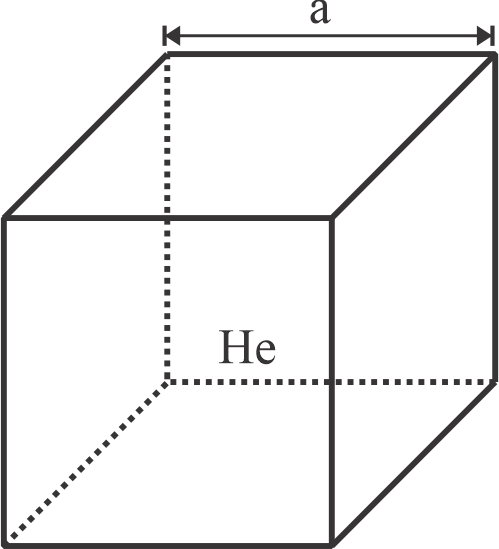
\includegraphics[width=3.5cm]{imagenes/general2024-I/etapa2/ing/quimica-1.png}
		\vspace{6mm}
		\end{minipage}
		\hfill
		\begin{minipage}{0.45\textwidth}
			\centering
			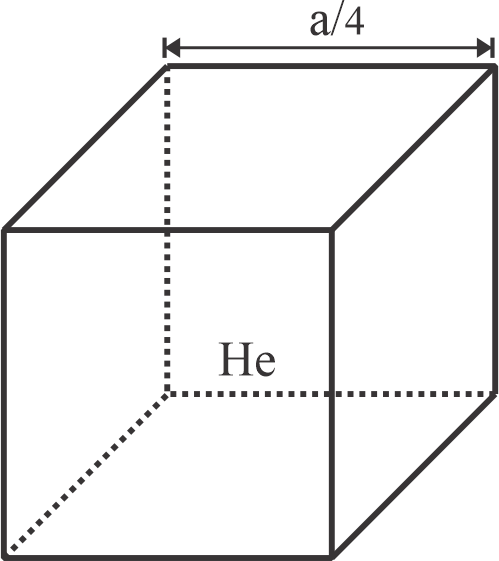
\includegraphics[width=2cm]{imagenes/general2024-I/etapa2/ing/quimica-1.1.png}
		\end{minipage}
	\end{center}
	
	
	
	\begin{center}
		\begin{minipage}{0.45\textwidth}
				
			$V_1 = a^3$ 
			
			$P_1 = 2400$ 
			
			$T_1 = T$
			\vspace{6mm}
		\end{minipage}
		\hfill
		\begin{minipage}{0.45\textwidth}
			$V_2 = \left(\dfrac{a}{4}\right)^3$\\
			$P_2 = ?$\\
			$T_2 = 0,4T$
		\end{minipage}
	\end{center}
	
	
	Utilizamos la ecuación general de los gases ideales:
	
	$\dfrac{P_1 V_1}{T_1} = \dfrac{P_2 V_2}{T_2}$
	
	$\dfrac{(2400)(a^3)}{T} = \dfrac{P_2 \cdot \left(\dfrac{a}{4}\right)^3}{0,4T}$
	
	$\Rightarrow (0,4T)(2400)(a^3) = \dfrac{P_2 (a^3) T}{64}$
	
	$\Rightarrow$ \fbox{ $P_2 = 61440 \, \text{mm Hg}$}
	
	\vspace{6mm}
	
	\item ¿Cuántos segundos debe transcurrir para que una corriente de $120 \, \text{A}$ deposite en el cátodo $5 \, \text{g}$ de hierro ($\text{Fe}$) de una solución de cloruro de hierro(III), $\text{FeCl}_3$?
	
	($1 \, \text{Faraday} = 96\,500 \, \text{Coulomb} \quad ; \quad \text{PA}(\text{Fe}) = 56$)
	\begin{enumerate}[label=\alph*)]
		\item 25,4
		\item 235,5
		\item 96,5
		\item 215,4
		\item 155,4
	\end{enumerate}
	\textbf{Respuesta correcta:} d)
	
	\vspace{2mm}
	\textbf{Solucionario:}\\
	
	Datos\\
	$I = 120 \, \text{A}$
	
	$t = ?$
	
	$m = 5 \, \text{g}$
	
	$\text{PA Fe} = 56$
	
	$\text{Farad} = 96\,500 \, \text{coulombios}$
	
	$\Rightarrow$ Utilizando ley de Faraday
	
	
	$m = \dfrac{P_{eq} \cdot I \cdot t}{96\,500}$ , despejando tiempo $t = \dfrac{96\,500 \cdot m}{P_{eq} \cdot I}$
	
	
	$t = \dfrac{(96\,500)(5)}{\left( \dfrac{56}{3} \right) \cdot 120}$ $\Rightarrow$ \fbox{$ t = 215,4 \, \text{s}$}
	

	\item ¿Qué masa de óxido de calcio se obtendrá si se calcina 1 tonelada de caliza, cuyo contenido de $C_aCO_3$ es del $62\%?  (C_a = 40;C=12;O=16)$\\
	$C_aCO_{3(s)}+calor \Rightarrow  C_aO_{(s)}+CO_{2(g)}$
	
	\begin{enumerate}[label=\alph*)]
		\item 347,2
		\item 233,4
		\item 374,0
		\item 185,8
		\item 620,0
	\end{enumerate}
	
	\textbf{Respuesta correcta:} a)
	
	\vspace{2mm}
	\textbf{Solucionario:}
	
	\textbf{Datos}
	
	$M_{CaO} = ?$
	
	Pureza $CaCO_3 = 62\%$
	
	1 Tonelada = $1000 \, kg$
	
	$ PM \, CaCO_3 = 100$
	
	$PM \, CaO = 56$
	
	Si la caliza tiene una pureza de $62\%$, entonces:\\
	$CaCO_3 = 1000 \, kg \times 62\%$\\
	$CaCO_3 = 620 \, kg$ puro\\
	
	$\Rightarrow \quad CaCO_3 \xrightarrow{\hspace{1cm}} CaO$\\
	\phantom{$\Rightarrow \quad$} $100 \xrightarrow{\hspace{1cm}} 56$\\
	\phantom{$\Rightarrow \quad$} $620 \xrightarrow{\hspace{1cm}} X$\\

	$X = \dfrac{(620)(56)}{100}$\\
	
	\fbox{
		$X = 347,2 \, g \, CaO$
	}
	
	
	\item Señale la suma de coeficientes de los productos en la siguiente reacción química:
	
	$CrI_3 + Cl_2 + KOH \rightarrow KIO_4 + K_2CrO_4 + KCl + H_2O$
	
	\begin{enumerate}[label=\alph*)]
		\item 65
		\item 46
		\item 39
		\item 94
		\item 87
	\end{enumerate}
	\textbf{Respuesta correcta:} d)
	
	\vspace{2mm}
	\textbf{Solucionario:}
	
	Asignamos estados de oxidación:
	
	En $CrI_3$:
	
	$Cr=+3$
	
	$I=-1$
	
	En $KIO_4$:
	
	$I+4(-2)+1=0$
	
	$I-8+1=0$
	
	$I=+7$
	
	En $K_2CrO_4$:
	
	$Cr+4(-2)+2(+1)=0$
	
	$Cr-8+2=0$
	
	$Cr=+6$
	
	
	$Cr^{+3}\rightarrow Cr^{+6}$
	
	Pierde $3e^-$
	
	$I^{-1}\rightarrow I^{+7}$
	
	Pierde $8e^-$
	
	$Cl_2^{0}\rightarrow Cl^{-1}$
	
	Gana $2e^-$
	
	
	$2CrI_3+27Cl_2+64KOH\rightarrow 6KIO_4+2K_2CrO_4+54KCl+32H_2O$
	
	La suma de coeficientes de los productos es:
	
	$6+2+54+32=94$
	
	\fbox{$94$}
	
	\vspace{6mm}
	
	
	
	
\end{enumerate}	
	
	
	
	\subsection*{Biología y Anatomía}
	
	\begin{enumerate}[resume]
		
		\item las plantas que crecen cerca del agua y en suelos muy húmedos con provisión de agua permanente, como los musgos y helechos se denominan:
		
		\begin{enumerate}[label=\alph*)]
			\item halofitas.
			\item psicrofitas.
			\item higrófitas.
			\item xenófitas.
			\item hidrofitas.
		\end{enumerate}
		
		\textbf{Respuesta correcta:} c)
		
	\vspace{2mm}
	\textbf{Solucionario:}\\[1mm]
	
	Las higrófitas son plantas que se desarrollan en ambientes con alta humedad y con disponibilidad permanente de agua, como riberas, pantanos y suelos constantemente húmedos. Ejemplos típicos son los musgos y helechos, los cuales requieren condiciones húmedas para su crecimiento y reproducción.
	No viven totalmente sumergidas, a diferencia de las hidrófitas.
		
		\vspace{6mm}
		
		\item Son peces vertebrados sin mandíbulas, carecen de escamas y tienen una piel mucosa resbaladiza.
		\begin{enumerate}[label=\alph*)]
			\item Condrictios
			\item Gnatostomados
			\item Osteíctios
			\item Tunicados
			\item Agnatos
		\end{enumerate}
		
		\textbf{Respuesta correcta:} e)
		
			\vspace{2mm}
		\textbf{Solucionario:}
		
		Los agnatos son vertebrados primitivos caracterizados por carecer de mandíbulas, escamas y aletas pares. Presentan una piel mucosa resbaladiza y una boca circular adaptada para succión. Ejemplos representativos son las lampreas y mixinos, considerados los peces más antiguos.
		
		\vspace{6mm}
		
	\end{enumerate}
	

\subsection*{Psicología y Filosofía}

\begin{enumerate}[resume]
	
	\item Claudia le dice a su mamá: ¡La ropa de caperucita es muy bonita!, mientras esta le lee el cuento.
	¿Qué tipo de imaginación está utilizando Claudia?
	
	\begin{enumerate}[label=\alph*)]
		\item Creadora
		\item Reproductora
		\item Icónica
		\item Alucinación
		\item Fantástica
	\end{enumerate}
	
	\textbf{Respuesta correcta:} b)
	
      \vspace{2mm}
      \textbf{Solucionario:}\\
      
      La imaginación reproductora consiste en recrear mentalmente imágenes ya conocidas, a partir de relatos, lecturas o experiencias previas.
      Claudia imagina la vestimenta de Caperucita Roja basándose en el cuento que está escuchando, sin crear elementos nuevos, por lo que no se trata de una imaginación creadora o fantástica.
	
	\vspace{6mm}
	
	\item Rebeca le dice a su hijo: "Cuando termines la tarea te llevaré al cine. En el acto, Rebeca, para controlar el comportamiento de su hijo, utiliza el:
	\begin{enumerate}[label=\alph*)]
		\item reforzamiento positivo.
		\item castigo negativo.
		\item castigo positivo.
		\item reforzamiento continuo.
		\item reforzamiento negativo.
	\end{enumerate}
	
	\textbf{Respuesta correcta:} a)
	

	\vspace{2mm}
	\textbf{Solucionario:}\\
	
 El reforzamiento positivo consiste en presentar un estímulo agradable (ir al cine) para incrementar una conducta deseada (hacer la tarea).
 Rebeca motiva a su hijo ofreciéndole una recompensa, lo cual aumenta la probabilidad de que cumpla con la tarea.
	
	
	
	\item El escéptico \underline{\hspace{1.5cm}} la posibilidad del conocimiento pleno.
	
	\begin{enumerate}[label=\alph*)]
		\item afirma
		\item niega
		\item prueba
		\item comprueba
		\item critica
	\end{enumerate}
	
	\textbf{Respuesta correcta:} b)
	
	
	\vspace{2mm}
	\textbf{Solucionario:}\\
	
	El escepticismo es una corriente filosófica que niega o duda de la posibilidad de alcanzar un conocimiento verdadero y absoluto.
	El escéptico sostiene que el ser humano no puede conocer la realidad de manera plena y definitiva, por lo que adopta una actitud de duda constante.


	\vspace{6mm}
	
	\item Es el conocimiento práctico de las cosas, basado en la experiencia personal, arbitrario y carente de fundamentación.
	\begin{enumerate}[label=\alph*)]
		\item conocimiento filosófico
		\item conocimiento científico
		\item conocimiento vulgar
		\item conocimiento conceptual
		\item conocimiento metafisíco
	\end{enumerate}
	
	\textbf{Respuesta correcta:} c)
		
		
		\vspace{2mm}
		\textbf{Solucionario:}\\
	
		El conocimiento vulgar (o empírico) es aquel que se adquiere a través de la experiencia cotidiana, sin método ni fundamentación científica.
		Es subjetivo, asistemático y arbitrario, pero útil para la vida diaria, ya que permite desenvolverse en situaciones comunes.
		
		
	\vspace{6mm}
		
\end{enumerate}





\subsection*{Geografía}

\begin{enumerate}[resume]
	
	\item De acuerdo al MINAM, ¿qué instrumento técnico se requiere para desarrollar el ordenamiento territorial?
	
	\begin{enumerate}[label=\alph*)]
		\item La estrategia global para la sostenibilidad
		\item La Zonificación Ecológica y Económica
		\item El estudio no especializado
		\item El levantamiento topográfico
		\item La caracterización de imágenes satelitales
	\end{enumerate}
	
	\textbf{Respuesta correcta:} b)
	
	\vspace{2mm}
	\textbf{Solucionario:}\\[1mm]
	El Ministerio del Ambiente (MINAM) establece que la Zonificación Ecológica y Económica (ZEE) es el principal instrumento técnico para el ordenamiento territorial.
	La ZEE permite identificar las potencialidades y limitaciones del territorio, considerando criterios físicos, biológicos, sociales, económicos y culturales, con el fin de orientar el uso sostenible del territorio y la toma de decisiones públicas y privadas.
	
	\vspace{6mm}
	
	\item En el Perú, \dots\dots\dots\dots\dots son áreas destinadas a la conservación de la diversidad biológica y a la utilización sostenible de los recursos de flora y fauna silvestre, con excepción de la explotación forestal comercial, en el marco de la clasificación de áreas naturales protegidas (ANP)
	\begin{enumerate}[label=\alph*)]
		\item los Parques nacionales
		\item los Bosques de protección
		\item las Reservas comunales
		\item las Reservas nacionales
		\item las Zonas reservadas
	\end{enumerate}
	
	\textbf{Respuesta correcta:} d)
	
		\vspace{2mm}
	\textbf{Solucionario:}\\[1mm]
	En el Perú, las Reservas Nacionales son un tipo de Área Natural Protegida (ANP) destinadas a la conservación de la diversidad biológica, donde se permite el aprovechamiento sostenible de los recursos naturales, excepto la explotación forestal maderable comercial.
	Estas actividades deben realizarse bajo planes de manejo y supervisión del Estado, garantizando la sostenibilidad de los ecosistemas.
	
	\vspace{6mm}
	
\end{enumerate}



\subsection*{Historia}

\begin{enumerate}[resume]
	
\item Para realizar cálculos matemáticos, los incas utilizaron un instrumento denominado:

\begin{enumerate}[label=\alph*)]
	\item tocapu.
	\item quipu.
	\item yupana.
	\item ushnu.
	\item urpo.
\end{enumerate}

\textbf{Respuesta correcta:} c)

\vspace{2mm}
\textbf{Solucionario:}\\[1mm]
La yupana era un dispositivo utilizado por los incas (una especie de ábaco) para realizar operaciones aritméticas complejas. Aunque el quipu se usaba para la contabilidad y registro de datos, la yupana era la herramienta específica para el cálculo.

\vspace{6mm}

\item La cultura romana exaltó los triunfos a través de monumentos arquitectónicos conocidos como:

\begin{enumerate}[label=\alph*)]
	\item esculturas.
	\item pórticos.
	\item obeliscos.
	\item arcos.
	\item columnas.
\end{enumerate}

\textbf{Respuesta correcta:} d)

\vspace{2mm}
\textbf{Solucionario:}\\[1mm]
Los Arcos de Triunfo eran estructuras monumentales construidas por los romanos para conmemorar victorias militares y honrar a sus generales o emperadores.


	
	\vspace{6mm}
	
\end{enumerate}


\subsection*{Educación Cívica}

\begin{enumerate}[resume]
	

	\vspace{2mm}	

	\item Es el responsable de velar por el mantenimiento de la moral pública, perseguir y prevenir el delito y promover la reparación civil en favor de las personas que son lesionadas en sus derechos e intereses.
	
	\begin{enumerate}[label=\alph*)]
		\item Tribunal Constitucional
		\item Ministerio Público
		\item Fuerzas Armadas
		\item Poder Judicial
		\item Poder Ejecutivo
	\end{enumerate}
	
	\textbf{Respuesta correcta:} b)
	
	\vspace{2mm}
	\textbf{Solucionario:}\\[1mm]
	El Ministerio Público es el organismo autónomo del Estado que tiene como funciones principales la defensa de la legalidad y de los intereses públicos tutelados por el derecho, así como la persecución del delito y la reparación civil de las víctimas.
	
	\vspace{6mm}
	
	\item El Secretario General de la OEA y la ONU son elegidos por un periodo de:
	
	\begin{enumerate}[label=\alph*)]
		\item cuatro y cinco años respectivamente.
		\item cinco y cuatro años respectivamente.
		\item cinco años para cada Secretario General.
		\item cuatro años para cada Secretario con posibilidad de reelección.
		\item cuatro años sin posibilidad de reelección.
	\end{enumerate}
	
	\textbf{Respuesta correcta:} c)
	
	\vspace{2mm}
	\textbf{Solucionario:}\\[1mm]
	
	Tanto el Secretario General de la Organización de los Estados Americanos (OEA) como el de la Organización de las Naciones Unidas (ONU) son elegidos para ejercer sus funciones por un periodo de cinco años.

	
	\vspace{6mm}
	
\end{enumerate}


\subsection*{Economía}

\begin{enumerate}[resume]
	
\item En una economía de mercado, si la inflación subió en forma inesperada por encima de lo proyectado; entonces, los salarios se \underline{\hspace{2cm}} y los beneficios se \underline{\hspace{2cm}}.

\begin{enumerate}[label=\alph*)]
	\item incrementan - reducen.
	\item indexan - distribuyen.
	\item reducen - incrementan.
	\item reducen - reducen.
	\item incrementan - incrementan.
\end{enumerate}

\textbf{Respuesta correcta:} d)

\vspace{2mm}
\textbf{Solucionario:}\\[1mm]

En un escenario de inflación inesperada, los salarios reales se reducen porque pierden poder adquisitivo frente al alza de precios. Asimismo, los beneficios reales de las empresas también pueden verse reducidos debido a la incertidumbre económica, el aumento en los costos de los insumos y la caída en la demanda real de los consumidores.

\vspace{6mm}

\item En un determinado mercado, las funciones de demanda y oferta para una mercancía son:
\[ Q_x^d = 40 - 0,7Px \]
\[ Q_x^s = 10 + 0,3Px \]

Al precio de S/ 10 cada uno, se puede afirmar que en el mercado:

\begin{enumerate}[label=\alph*)]
	\item abunda la mercadería.
	\item sobran 10 unidades.
	\item faltan 20 unidades.
	\item sobran 30 unidades.
	\item faltan 40 unidades.
\end{enumerate}

\textbf{Respuesta correcta:} c)

\vspace{2mm}
\textbf{Solucionario:}\\[1mm]
Reemplazamos el precio ($Px = 10$) en ambas funciones:
\begin{itemize}
	\item Cantidad demandada: $Q_d = 40 - 0,7(10) = 40 - 7 = 33$
	\item Cantidad ofertada: $Q_s = 10 + 0,3(10) = 10 + 3 = 13$
\end{itemize}
Como la demanda ($33$) es mayor que la oferta ($13$), existe un exceso de demanda de $33 - 13 = 20$ unidades. Por lo tanto, faltan 20 unidades.


\vspace{6mm}
	
\end{enumerate}



\subsection*{Comunicación}

\begin{enumerate}[resume]
	
\item Escuché la voz de mi padre diciéndome "Mira Jaime ese es el Capitán", mientras señalaba al jugador que llevaba un brazalete al lado derecho.

En el fragmento, predomina el texto:

\begin{enumerate}[label=\alph*)]
	\item instructivo.
	\item descriptivo.
	\item narrativo.
	\item argumentativo.
	\item expositivo.
\end{enumerate}

\textbf{Respuesta correcta:} c)

\vspace{2mm}
\textbf{Solucionario:}\\[1mm]
El texto es narrativo porque relata un suceso o acción en un tiempo y espacio determinados (la acción de escuchar al padre y observar al jugador), presentando una secuencia de hechos.

\vspace{6mm}

\item Los sustantivos que nombran seres reales que pueden ser percibidos por nuestros sentidos y, por tanto, ser tocados, vistos, medidos, se denominan:

\begin{enumerate}[label=\alph*)]
	\item Propios.
	\item Concretos.
	\item Abstractos.
	\item Individuales.
	\item Colectivos.
\end{enumerate}

\textbf{Respuesta correcta:} b)

\vspace{2mm}
\textbf{Solucionario:}\\[1mm]
Los sustantivos concretos designan objetos o seres que tienen existencia física y real, los cuales pueden ser captados a través de los sentidos (vista, tacto, oído, etc.).

\vspace{6mm}

\item Como actuar en caso de accidente de tránsito:\\
1.- Cubra con ropas al lesionado para mantener su temperatura.\\
2.- Prevenga el shock.\\
3.- Controle la hemorragia, si la hay.\\
4.- Asegúrese de que el herido se mantenga respirando.

El propósito comunicativo del texto es:

\begin{enumerate}[label=\alph*)]
	\item advertir.
	\item convencer.
	\item deleitar.
	\item informar.
	\item mostrar.
\end{enumerate}

\textbf{Respuesta correcta:} a)

\vspace{2mm}
\textbf{Solucionario:}\\[1mm]
El texto tiene una función apelativa o exhortativa; su propósito es advertir y dar pautas de comportamiento o instrucciones necesarias para actuar ante una situación de emergencia.

\vspace{6mm}

\item Una obra literaria, en el proceso comunicativo, constituye el:

\begin{enumerate}[label=\alph*)]
	\item emisor.
	\item mensaje.
	\item código.
	\item receptor.
	\item contexto.
\end{enumerate}

\textbf{Respuesta correcta:} b)

\vspace{2mm}
\textbf{Solucionario:}\\[1mm]
Dentro del proceso de comunicación, la obra literaria es el contenido o la información que el autor (emisor) transmite al lector (receptor), por lo tanto, constituye el mensaje.

\vspace{6mm}
	
\end{enumerate}


\subsection*{Literatura}

\begin{enumerate}[resume]

\item Escribió poemas bajo el título \textit{Rimas}, 22 leyendas y una colección de prosas con el título \textit{Cartas desde mi Celda}.

\begin{enumerate}[label=\alph*)]
	\item Miguel de Cervantes Saavedra
	\item Tirso de Molina
	\item Francisco de Quevedo
	\item Gustavo Adolfo Bécquer
	\item Pedro Calderón de la Barca
\end{enumerate}

\textbf{Respuesta correcta:} d)

\vspace{2mm}
\textbf{Solucionario:}\\[1mm]

Gustavo Adolfo Bécquer es la figura máxima del Romanticismo tardío español. Su fama reside principalmente en sus \textit{Rimas}, poemas breves de tono melancólico, y sus \textit{Leyendas}, narraciones fantásticas en prosa. Escribió \textit{Cartas desde mi celda} durante su estancia en el monasterio de Veruela.

\vspace{6mm}

\item Mariátegui, a diferencia de otros intelectuales, consideró que al problema del indio era de carácter:

\begin{enumerate}[label=\alph*)]
	\item religioso
	\item educativo
	\item económico
	\item político
	\item moral
\end{enumerate}

\textbf{Respuesta correcta:} c)

\vspace{2mm}
\textbf{Solucionario:}\\[1mm]
En sus \textit{7 ensayos de interpretación de la realidad peruana}, José Carlos Mariátegui sostiene que el problema del indio no es pedagógico, moral ni jurídico, sino que tiene raíces económicas vinculadas a la propiedad de la tierra (el problema agrario y el gamonalismo).

\vspace{6mm}


\end{enumerate}






\subsection*{Razonamiento Matemático}

\begin{enumerate}[resume]



\item Si la suma de las fechas de todos los viernes de un determinado mes es igual a 85, ¿qué día cae el 15 de dicho mes?

\begin{enumerate}[label=\alph*)]
	\item Martes
	\item Miércoles
	\item Jueves
	\item Viernes
	\item Lunes
\end{enumerate}

\textbf{Respuesta correcta:} b)

\vspace{2mm}
\textbf{Solucionario:}

Las fechas de un mismo día de la semana forman una progresión aritmética de razón 7:

sea el primer viernes $= a$

 $a, a+7, a+14, a+21, a+28$.
 
Si sumamos 5 viernes: 

$5a + 70 = 85 \Rightarrow 5a = 15 \Rightarrow a = 3$.

Los viernes son: 3, 10, 17, 24 y 31.

Si el viernes es 17, retrocedemos dos días para llegar al 15: el día es miercoles.

\vspace{6mm}

\item Pamela con todas las monedas que tiene, forma un arreglo triangular de la siguiente manera: en la primera fila 1 moneda, en la segunda fila 2 monedas y sobre cada una de ellas una más, en la tercera fila tres monedas y sobre cada una de ellas 2 monedas más y así sucesivamente. Si pudo formar 20 filas en total, ¿cuántas monedas tenía?

\begin{enumerate}[label=\alph*)]
	\item 2790
	\item 2890
	\item 2870
	\item 2320
	\item 5740
\end{enumerate}

\textbf{Respuesta correcta:} c)

\vspace{2mm}
\textbf{Solucionario:}

Número de monedas por fila ($f$):

Fila 1: $1 \times 1 = 1^2$

Fila 2: $2 \times 2 = 2^2$

Fila 3: $3 \times 3 = 3^2$

Total para 20 filas:

$\sum_{i=1}^{20} i^2 = \dfrac{n(n+1)(2n+1)}{6}$

$S = \dfrac{20(21)(41)}{6} = 10(7)(41) = $\fbox{$2870$ monedas.}

\vspace{6mm}


\item Se compra un televisor en 630 soles. ¿Cuánto debo aumentar a este precio para que durante la venta se realice una rebaja de 10\% y así gane el 40\% del precio de costo?

\begin{enumerate}[label=\alph*)]
	\item S/ 250
	\item S/ 252
	\item S/ 350
	\item S/ 98
	\item S/ 198
\end{enumerate}

\textbf{Respuesta correcta:} c)

\vspace{2mm}
\textbf{Solucionario:}\\[1mm]
Sea $10x$ el aumento total sobre el costo. La rebaja es el $10\%$ de este aumento, es decir, $x$.
\begin{itemize}
	\item Precio de costo ($P_c$) = S/ 630
	\item Ganancia esperada ($40\% P_c$) = $0,40 \times 630$ = S/ 252
	\item Dinero a recibir = $P_c + \text{Ganancia} = 630 + 252 = 882$
\end{itemize}
Si el aumento total es $10x$ y se rebaja $x$, el dinero recibido equivale a $9x$:\\
$9x = 882 \Rightarrow x = 98$.\\
El costo a incrementar total es la Ganancia + Rebaja: $252 + 98 = \text{S/ 350}$.\\

\vspace{6mm}

\vspace{6mm}
\item Sabiendo que $\overline{UNA} + \overline{ANU} = 988$ y $U - A = 4$, calcule $N + A$.

\begin{enumerate}[label=\alph*)]
	\item 10
	\item 14
	\item 11
	\item 13
	\item 18
\end{enumerate}

\textbf{Respuesta correcta:} c)

\vspace{2mm}
\textbf{Solucionario:}

De la suma en unidades: $A + U = 8$.

Como $U - A = 4$, sumamos ambas: $(A+U) + (U-A) = 8 + 4 \Rightarrow 2U = 12 \Rightarrow U=6$.

Entonces $A = 2$.

En las decenas: $N + N = 18 \Rightarrow 2N = 18 \Rightarrow N = 9$.

Piden $N + A = 9 + 2 = 11$.

\vspace{6mm}

	\item En el cuadrado ABCD, cuyo lado mide 4 cm, determine el área de la región sombreada, siendo O el centro de la circunferencia.
	
		\begin{center}
		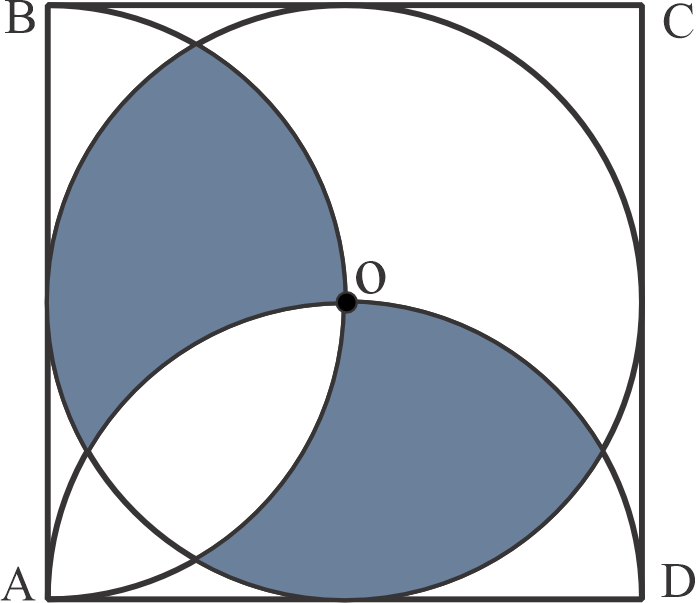
\includegraphics[width=3.5cm]{imagenes/general2024-I/etapa2/ing/rm5.png}\par\vspace{2cm}
	\end{center}
	
	
	
\begin{enumerate}[label=\alph*)]
	\item 4,0 \( \pi cm^2\)
	\item 3,5 \( \pi cm^2\)
	\item 3,0 \( \pi cm^2\)
	\item 2,5 \( \pi cm^2\)
	\item 2,0 \( \pi cm^2\)
\end{enumerate}

\textbf{Respuesta correcta:} e)

\vspace{2mm}
\textbf{Solucionario:}

	\begin{center}
	\begin{minipage}{0.45\textwidth}
	Al trazar $\overline{OM}$ y $\overline{ON}$, se observan regiones equivalentes, a cuyas áreas les asignamos los valores $a$ y $b$.\\
	piden $A_{somb}=2a+2b=??$\\
	Pero, del gráfico, $a+b=A_{DOND}=\dfrac{\pi 2^2}{4}=\pi\,cm^2$.\\
	$\therefore\ A_{somb}=2(a+b)=2\pi\,cm^2$\\

		\vspace{6mm}
	\end{minipage}
	\hfill
	\begin{minipage}{0.45\textwidth}
		\centering
		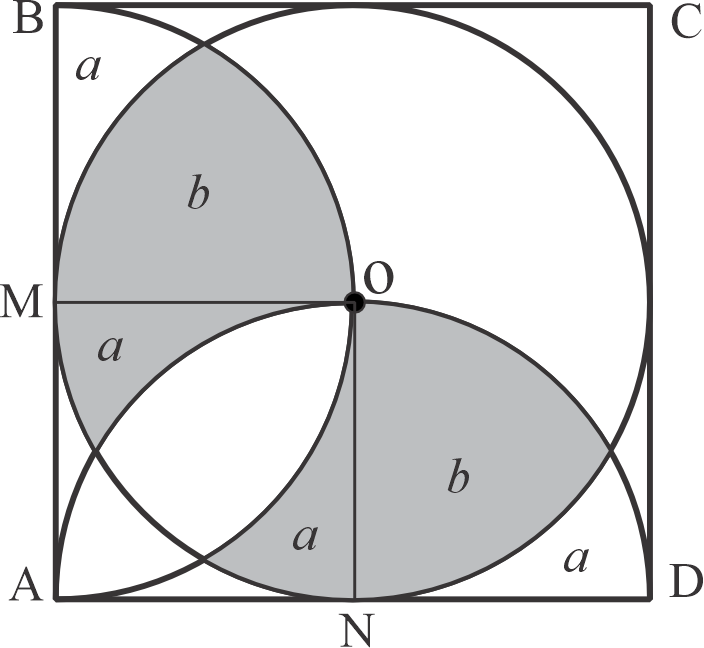
\includegraphics[width=3.5cm]{imagenes/general2024-I/etapa2/ing/rrm5.png}
	\end{minipage}
	\end{center}

\vspace{5mm}

\item El segundo término de una progresión aritmética es 7 y el séptimo término es 22. Halle la suma de los 100 primeros términos de la progresión.

\begin{enumerate}[label=\alph*)]
	\item 14250
	\item 15250
	\item 14350
	\item 15350
	\item 13250
\end{enumerate}

\textbf{Respuesta correcta:} b)

\vspace{2mm}
\textbf{Solucionario:}
$a_7 = a_2 + 5r \Rightarrow 22 = 7 + 5r \Rightarrow r = 3$.

Hallamos $a_1$: $a_2 = a_1 + r \Rightarrow 7 = a_1 + 3 \Rightarrow a_1 = 4$.

Hallamos $a_{100}$: $a_{100} = 4 + 99(3) = 301$.

Suma: $S_{100} = \dfrac{(4 + 301)100}{2} = 305 \times 50 = 15250$.



\end{enumerate}




\subsection*{Razonamiento Verbal}

\begin{enumerate}[resume]
	
\item El término que no corresponde a la palabra PARAFRASEAR es:

\begin{enumerate}[label=\alph*)]
	\item comentar.
	\item agilizar.
	\item argumentar.
	\item explicar.
	\item interpretar.
\end{enumerate}

\textbf{Respuesta correcta:} b)

\vspace{2mm}
\textbf{Solucionario:}\\[1mm]
Parafrasear consiste en explicar o interpretar un texto con palabras propias para hacerlo más comprensible. Términos como comentar, argumentar o explicar están ligados a este proceso cognitivo; sin embargo, "\text{agilizar}" no guarda relación semántica con la acción de traducir o explicar un contenido.

\vspace{6mm}

\item El sinónimo de la palabra PERORATA es:

\begin{enumerate}[label=\alph*)]
	\item discursivo.
	\item exordio.
	\item explicación.
	\item doctrina.
	\item alusión.
\end{enumerate}

\textbf{Respuesta correcta:} a)

\vspace{2mm}
\textbf{Solucionario:}\\[1mm]
Una perorata es un discurso o razonamiento, generalmente largo y aburrido, que se pronuncia ante un público. Por ello, el término \textbf{discursivo} es el que más se aproxima a la naturaleza de la palabra, aunque habitualmente se utiliza el sustantivo "discurso".

\vspace{6mm}

\item Complete las oraciones.\\
A partir de la fabricación de la primera bomba atómica, \dots\dots\dots\dots\dots se ha hecho para salvar al mundo de la guerra, \dots\dots\dots\dots\dots se ha hecho mucho \dots\dots\dots\dots\dots aumentar su capacidad destructiva.

\begin{enumerate}[label=\alph*)]
	\item poco - y - al
	\item no - y tampoco - para
	\item algo - y - como para
	\item mucho - por el contrario - con el fin de
	\item nada - mientras - para
\end{enumerate}

\textbf{Respuesta correcta:} e)

\vspace{2mm}
\textbf{Solucionario:}\\[1mm]

La oración expresa una oposición temporal y de sentido entre dos acciones relacionadas con la bomba atómica.
En la primera parte, se indica que no se ha hecho nada para salvar al mundo de la guerra; mientras que en la segunda parte se señala que sí se ha actuado con un propósito, es decir, para aumentar su capacidad destructiva.

El conector “mientras” introduce un contraste simultáneo, mostrando que, al mismo tiempo que no se realizan acciones para la paz, se desarrollan acciones orientadas a la destrucción.
La preposición “para” expresa finalidad, indicando el objetivo de aumentar el poder destructivo.

Por ello, la alternativa que mantiene coherencia lógica y semántica es:

\vspace{6mm}

\item Identifica el par analógico.\\
INGENIERO : MINA ::

\begin{enumerate}[label=\alph*)]
	\item aviador : cosmos.
	\item peregrino : agua.
	\item citadino : campo.
	\item marino : lago.
	\item geólogo : montaña.
\end{enumerate}

\textbf{Respuesta correcta:} e)

\vspace{2mm}
\textbf{Solucionario:}\\[1mm]
La analogía es de Sujeto : Lugar de trabajo o acción. Un ingeniero desempeña sus funciones técnicas frecuentemente en una mina; del mismo modo, un geólogo realiza sus estudios de campo y análisis profesional predominantemente en la montaña.
	
	
	
	\item \textbf{PLAN DE REDACCIÓN}
	
	\begin{center}
		\textbf{Los Trenes}
	\end{center}
	
	I. El Ferrocarril Central del Perú es la línea férrea más alta del mundo y fue construido en 1873. \\
	II. La empresa Nacional de Ferrocarriles del Perú fue privatizada en 1996. \\
	III. El gobierno de Velasco Alvarado crea la Empresa Nacional de Ferrocarriles (ENAFER). \\
	IV. El primer tren del Perú se inauguró en 1852, fue el Lima – Callao y luego el Lima – Chorrillos. \\
	V. En los años veinte las carreteras desplazaron a los trenes en el Perú.
	
	\begin{enumerate}[label=\alph*)]
		\item IV - I - V - III - II
		\item IV - V - I - II - III
		\item III - V - I - IV - II
		\item I - IV - V - II - III
		\item I - V - II - III - IV
	\end{enumerate}
	
	\textbf{Respuesta correcta:} a)
	
	\vspace{2mm}
	\textbf{Solucionario:}\\[1mm]
	El criterio de ordenación es cronológico:\\
	1. (IV) 1852: Primer tren.\\
	2. (I) 1873: Ferrocarril Central.\\
	3. (V) Años veinte: Desplazamiento por carreteras.\\
	4. (III) Gobierno de Velasco (1968-1975): Creación de ENAFER.\\
	5. (II) 1996: Privatización.\\	
	
	
	\item La República del Perú es democrática, social, independiente y soberana. El Estado es uno e indivisible. Su gobierno es unitario representativo y descentralizado, y se organiza según el principio de la separación de poderes (Art. 43º C.P. 93).
	
	Lo descrito significa que:
	
	\begin{enumerate}[label=\alph*)]
		\item La Constitución Política tiene un carácter presidencialista.
		\item El Congreso de la República es el primer poder del Estado.
		\item Ningún poder del Estado tiene primacía sobre el otro.
		\item El equilibrio de poderes, parcialmente está garantizado.
		\item La hegemonía del Estado de Derecho está por encima de toda ley.
	\end{enumerate}
	
	\textbf{Respuesta correcta:} c)
	
	\vspace{2mm}
	\textbf{Solucionario:}\\[1mm]
	El principio de separación de poderes establece una estructura de "frenos y contrapesos" donde el Poder Ejecutivo, Legislativo y Judicial son autónomos e independientes entre sí. Esto garantiza que no exista una jerarquía de supremacía de un poder sobre los demás, buscando el equilibrio en el ejercicio del poder estatal.
	
	
	
	\vspace{6mm}
	
	
	
	\vspace{6mm}
	
\end{enumerate}




\subsection*{Inglés}

\begin{enumerate}[resume]

\item In the sentence: Lionel Messi is a famous soccer player.
What is the underlined word?

\begin{enumerate}[label=\alph*)]
	\item a verb.
	\item a preposition.
	\item a gerund.
	\item a noun.
	\item an adjective.
\end{enumerate}

\textbf{Respuesta correcta:} e)

\vspace{2mm}
\textbf{Solucionario:}\\[1mm]
La palabra "famous" (famoso) funciona como un adjetivo en la oración, ya que su función es calificar o describir una característica del sustantivo "soccer player".

\vspace{6mm}

\item If I say: just every Monday I do the laundry.
How often do I do the laundry?

\begin{enumerate}[label=\alph*)]
	\item twice a day
	\item once a week
	\item once a day
	\item ever Friday
	\item three times a day
\end{enumerate}

\textbf{Respuesta correcta:} b)

\vspace{2mm}
\textbf{Solucionario:}\\[1mm]
La expresión "every Monday" (cada lunes) indica una frecuencia semanal. Dado que el lunes ocurre una vez por semana, la respuesta correcta es "once a week".

\vspace{6mm}
\end{enumerate}





\subsection*{Quechua y Aimara}

\begin{enumerate}[resume]



\item ¿Hayk'a k'uchukunayuqtaq wasi punkuri kan? / ¿Qawqha k'uchukananisa uta punkuxa?

\begin{enumerate}[label=\alph*)]
	\item Iskay k'uchukunayuq / Pä k'uchukananiwa.
	\item Qanchis k'uchukunayuq / Paqallqu k'uchukananiwa.
	\item Kimsa k'uchukunayuq / Kimsa k'uchukananiwa.
	\item Tawa k'uchukunayuq / Pusi k'uchukananiwa.
	\item Pichqa k'uchukunayuq / Phisqa k'uchukananiwa.
\end{enumerate}

\textbf{Respuesta correcta:} d)

\vspace{2mm}
\textbf{Solucionario:}\\[1mm]
La pregunta inquiere cuántas esquinas o ángulos tiene la puerta de una casa. Al ser rectangular, la respuesta es cuatro: \textbf{Tawa} (quechua) / \textbf{Pusi} (aymara).

\vspace{6mm}

\item ¿Ima yupaytaq chunka tawayuq chawpinri? / ¿Kuna jakhusa tunka pusini chikatapaxa?

\begin{enumerate}[label=\alph*)]
	\item Suqta / Suxta
	\item Qanchis / Paqallqu
	\item Pusaq / Kimsaqallqu
	\item Isqun / Llatunka
	\item Chunka / Tunka
\end{enumerate}

\textbf{Respuesta correcta:} b)

\vspace{2mm}
\textbf{Solucionario:}\\[1mm]
Se pregunta por la mitad de catorce (chunka tawayuq / tunka pusini). La mitad es siete: \textbf{Qanchis} en quechua y \textbf{Paqallqu} en aymara.



\end{enumerate}










\section*{Área: Biomédicas}

\addcontentsline{toc}{subsection}{Área: Biomédicas}

\subsection*{Aritmética}

\begin{enumerate}
	
	\item Una familia está dedicada a la crianza de animales y ellos tienen $\overline{aba}$ animales. A causa de una epidemia se le mueren $\overline{ab}$ vacas, $\overline{10a}$ carneros y $\overline{b0}$ conejos, hasta que al final se quedan con $\overline{7(3a)}$ animales. Halle $5a-2b$.
	\begin{enumerate}[label=\alph*)]
		\item 0
		\item -3
		\item 5
		\item 2
		\item -1
	\end{enumerate}
	\textbf{Respuesta correcta:} d)
	
	\vspace{2mm}
	\textbf{Solucionario:}
	

	$\underbrace{\overline{aba}}_{\text{Total inicial}} - \underbrace{(\overline{ab} + \overline{10a} + \overline{b0})}_{\text{mueren}} = \underbrace{\overline{7(3a)}}_{\text{Total final}}$ 
	
	Como $3a \le 9$, entonces, $1 \le a \le 3$ 
	
	Descomponemos polinómicamente: 
	
	$100a + 10b + a - (10a + b + 100 + a + 10b) = 70 + 3a$ 
	
	$100a - 10a - b - 100 = 70 + 3a$ 
	
	$87a = 170 + b$; $b < 9$ 
	
	$\downarrow$ \hspace{6mm} $\downarrow$ 
	
	$2$ \hspace{7.5mm} $4$ 
	
	Luego $5a - 2b \implies 5(2) - 2(4) = 10 - 8 =$\fbox{$ 2$}
	
	\vspace{6mm}
	
	\item Tres ciclistas parten al mismo tiempo de un punto de una pista circular que tiene $240\text{ m}$ de circunferencia. El primero con velocidad de $8\text{ m/s}$, el segundo a $5\text{ m/s}$ y el tercero a $3\text{ m/s}$. ¿Cuánto tiempo transcurrirá para que los tres móviles realicen el primer encuentro?
	\begin{enumerate}[label=\alph*)]
		\item 8 min
		\item 2 min
		\item 4 min
		\item 10 min
		\item 12 min
	\end{enumerate}
	\textbf{Respuesta correcta:} c)
	
	\vspace{2mm}
	\textbf{Solucionario:}
	
	Calculamos el tiempo que emplea c/u en dar 1 vuelta: 
	
	$T_{1ro} = 240 \div 8 = 30\text{ s}$ 
	
	$T_{2do} = 240 \div 5 = 48\text{ s}$ 
	
	$T_{3ro} = 240 \div 3 = 80\text{ s}$ 
	
	El tiempo que emplean para encontrarse por primera vez deberá ser el: 
	
	$\text{MCM}(30, 48, 80) = 240\text{ s}$ 
	
	$240\text{ s} \implies $\fbox{$4\text{ min}$}
	
	\vspace{6mm}
	
	\item De un lote de 12 artículos se sabe que 8 no tienen ningún defecto. Si se toma al azar 3 artículos del lote, halle la probabilidad de que los 3 estén defectuosos.
	\begin{enumerate}[label=\alph*)]
		\item $\dfrac{1}{55}$
		\item $\dfrac{41}{55}$
		\item $\dfrac{14}{55}$
		\item $\dfrac{17}{77}$
		\item $\dfrac{5}{33}$
	\end{enumerate}
	\textbf{Respuesta correcta:} a)
	
	\vspace{2mm}
	\textbf{Solucionario:}
	
	Veamos:
	\begin{center}
		Total (12) $\rightarrow$ 4 con defecto / 8 sin defecto
	\end{center}
	La probabilidad de elegir tres artículos defectuosos de un total de 12 se calculará así: 
	
	
	$P = \dfrac{(n.^\circ \text{ de casos favorables})}{(n.^\circ \text{ de casos totales})}$ 
	
	$\implies P = \dfrac{C_{3}^{4}}{C_{3}^{12}} = \dfrac{\dfrac{4!}{3! \times 1!}}{\dfrac{12!}{3! \times 9!}} = \dfrac{4! \times 9!}{12!}$ 
	
	$P = \dfrac{24 \times 1}{10 \times 11 \times 12} = \dfrac{2}{110} = $\fbox{$\dfrac{1}{55}$}
	
	\vspace{6mm}
\end{enumerate}		







\subsection*{Álgebra}

\begin{enumerate}[resume]
	
	\item Si $(G \circ F)(x) = x + 2$ y $F(x) = x^3 + 6x^2 + 12x + 8$, halle $G(x)$.
	\begin{enumerate}[label=\alph*)]
		\item $G(x) = \sqrt[3]{x}$
		\item $G(x) = \sqrt{x}$
		\item $G(x) = \sqrt[3]{x^2}$
		\item $G(x) = \sqrt{x} + 2$
		\item $G(x) = \sqrt{x^3}$
	\end{enumerate}
	\textbf{Respuesta correcta:} a)
	
	\vspace{2mm}
	\textbf{Solucionario:}
	
	$(G \circ F)(x) = x + 2 \Rightarrow G(F(x)) = x + 2$
	
	$F(x) = x^3 + 6x^2 + 12x + 8$
	
	\hfill
	\begin{tabular}{c|cccc}
		& 1 & 6 & 12 & 8 \\
		-2 & & -2 & -8 & -8 \\
		\hline
		& 1 & 4 & 4 & 0
	\end{tabular}\\
	$= (x + 2)(x^2 + 4x + 4)$
	
	$= (x + 2)^3$
	
	luego
	
	$G((x + 2)^3) = x + 2 = \sqrt[3]{(x + 2)^3}$
	
	$G(X) =$\fbox{$ \sqrt[3]{x}$}
	
	\vspace{6mm}
	
	\item Si $A$ es una matriz que verifica:
	$(A + I)^2 = \begin{pmatrix} 4 & -3 \\ 3 & 2 \end{pmatrix}$ y $(A - I)^2 = \begin{pmatrix} -1 & 0 \\ 0 & -1 \end{pmatrix}$
	Halle la traza de $A$.
	\begin{enumerate}[label=\alph*)]
		\item 2
		\item 1
		\item 4
		\item 5
		\item 6
	\end{enumerate}
	\textbf{Respuesta correcta:} a)
	
	\vspace{2mm}
	\textbf{Solucionario:}
	
	$(A + I)^2 - (A - I)^2 = \begin{pmatrix} 4 & -3 \\ 3 & 2 \end{pmatrix} - \begin{pmatrix} -1 & 0 \\ 0 & -1 \end{pmatrix} = \begin{pmatrix} 5 & -3 \\ 3 & 3 \end{pmatrix}$
	
	$[A + I + A - I][A + I - A + I] = \begin{pmatrix} 5 & -3 \\ 3 & 3 \end{pmatrix}$
	
	$2A \cdot 2I = \begin{pmatrix} 5 & -3 \\ 3 & 3 \end{pmatrix} \Rightarrow A = \begin{pmatrix} \dfrac{5}{4} & \dfrac{-3}{4} \\ \dfrac{3}{4} & \dfrac{3}{4} \end{pmatrix}$
	
	Traza de $A = \dfrac{5}{4} + \dfrac{3}{4} = $\fbox{$2$}
	
	\vspace{6mm}
	
	\item Calcule:
	$E = \log_3(4 + \log_2 8 + \log_5 25)$
	\begin{enumerate}[label=\alph*)]
		\item 1
		\item 2
		\item 3
		\item 4
		\item 0
	\end{enumerate}
	\textbf{Respuesta correcta:} b)
	
	\vspace{2mm}
	\textbf{Solucionario:}
	
	$E = \log_3(4 + \log_2 8 + \log_5 25) = \log_3(4 + \log_2 2^3 + \log_5 5^2)$
	
	$= \log_3(4 + 3(1) + 2(1)) = \log_3(9)$
	
	\fbox{$= 2$}
	
	\vspace{6mm}
\end{enumerate}



\subsection*{Geometría}

\begin{enumerate}[resume]
	\item En la figura, halle $\dfrac{y}{x}$
	
	
	\begin{center}
		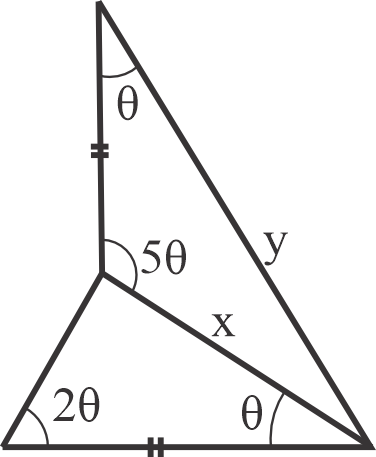
\includegraphics[width=3cm]{imagenes/general2024-I/etapa2/bio/geo1g24-II.png}
	\end{center}
	
	
	
	\begin{enumerate}[label=\alph*)]
		\item 3
		\item 1
		\item 2
		\item 4
		\item 5
	\end{enumerate}
	\textbf{Respuesta correcta:} c)
	
	\vspace{2mm}
	\textbf{Solucionario:}\\[1mm]
	
	
	
	\begin{center}
		\begin{minipage}{0.45\textwidth}
			Por congruencia de triangulos: \\
			
			De la figura se tiene:\\
			
			$2x=y$\\
			
			\fbox{$2$}$=\dfrac{y}{x}$
			
			\vspace{6mm}
		\end{minipage}
		\hfill
		\begin{minipage}{0.45\textwidth}
			\centering
			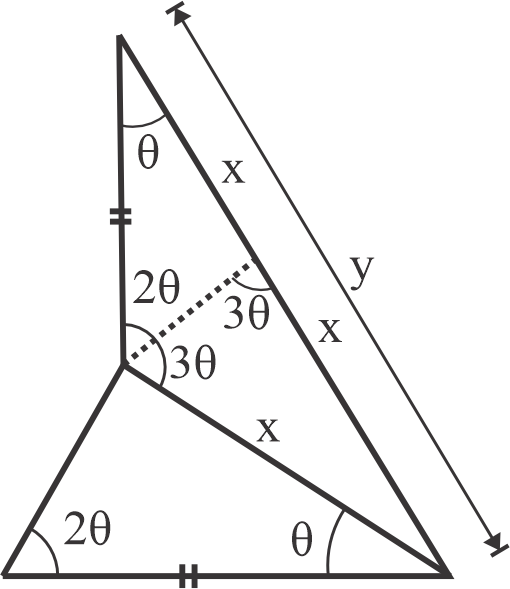
\includegraphics[width=3.5cm]{imagenes/general2024-I/etapa2/bio/geo1g24r-II.png}
		\end{minipage}
	\end{center}
	
	
	
	
	
	\vspace{6mm}
	
	\item En la figura,O es centro, UN=NA=$\sqrt{2}$ y P es Punto de Tangencia Calcule AP.
	
	\begin{center}
		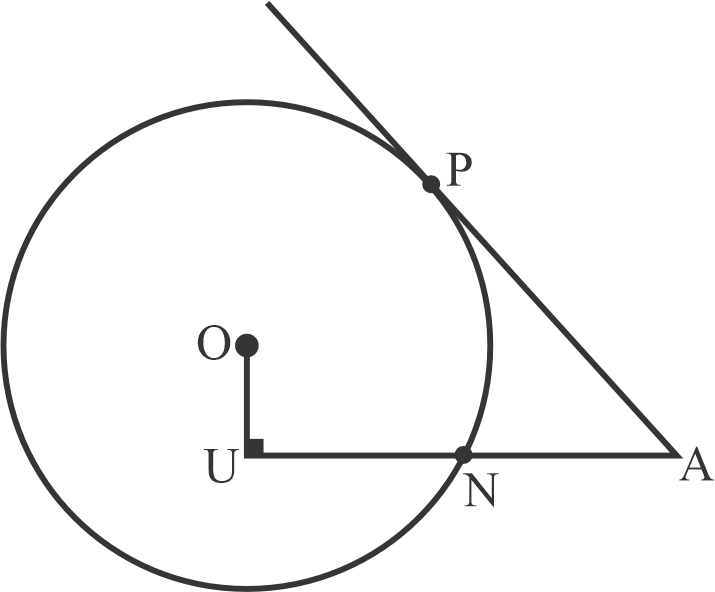
\includegraphics[width=4cm]{imagenes/general2024-I/etapa2/bio/geo2g24-II.png}
	\end{center}
	
	\begin{enumerate}[label=\alph*)]
		\item $\sqrt{3}$
		\item $\sqrt{6}$
		\item 3
		\item 6
		\item 5
	\end{enumerate}
	\textbf{Respuesta correcta:} b)
	
	\vspace{2mm}
	\textbf{Solucionario:}
	
	\begin{center}
		\begin{minipage}{0.45\textwidth}
			Por relaciones métricas \\
			
			$x^2=(3\sqrt{2})(\sqrt{2})$\\
			
			$x^2=3(2)$\\
			
			$x=$\fbox{$\sqrt{6}$}
			
			\vspace{6mm}
		\end{minipage}
		\hfill
		\begin{minipage}{0.45\textwidth}
			\centering
			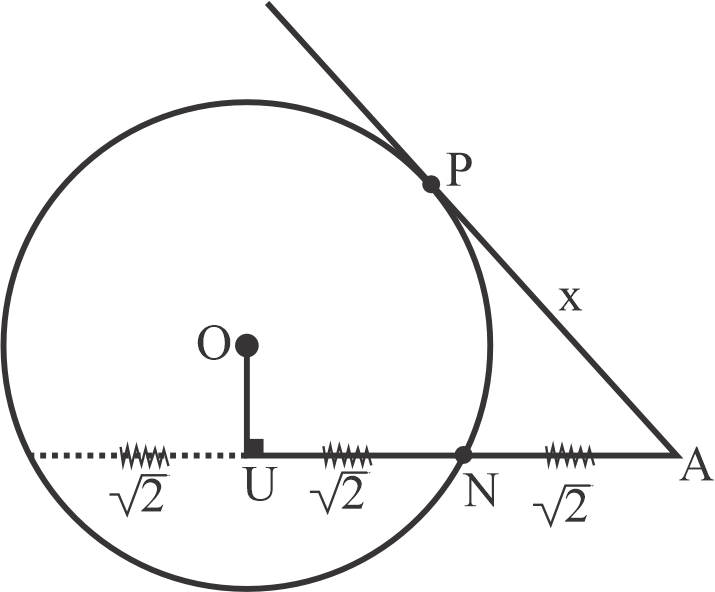
\includegraphics[width=4cm]{imagenes/general2024-I/etapa2/bio/geo2g24-IIr.png}
		\end{minipage}
	\end{center}
	
	
	\item En la figura, calcule AB.
	
	\begin{center}
		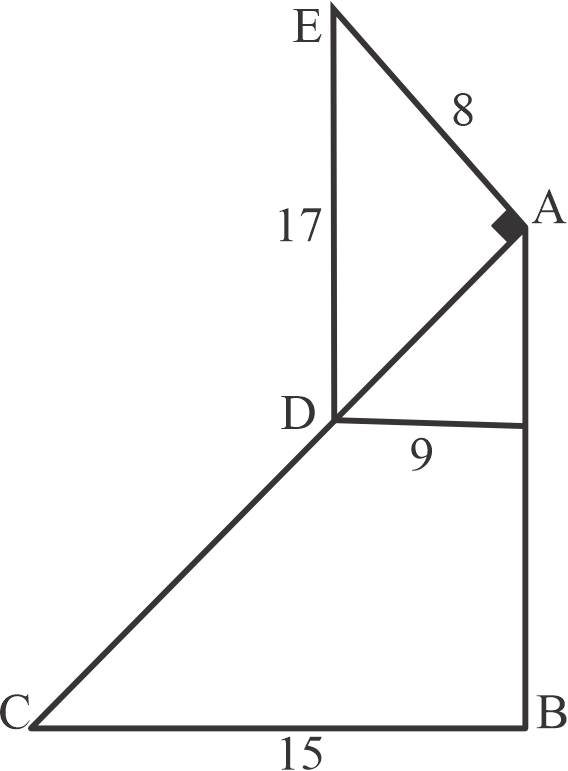
\includegraphics[width=3cm]{imagenes/general2024-I/etapa2/bio/geo3g24-II.png}
	\end{center}
	
	\begin{enumerate}[label=\alph*)]
		\item 14
		\item 15
		\item 16
		\item 18
		\item 20
	\end{enumerate}
	\textbf{Respuesta correcta:} c)
	
	\vspace{2mm}
	\textbf{Solucionario:}\\[1mm]
	
	\begin{center}
		\begin{minipage}{0.45\textwidth}
			Por semejanza de triángulos \\
			
			$\bigtriangleup APD \sim  \bigtriangleup ABC $\\
			
			$\dfrac{x}{12}=\dfrac{15}{9}$\\
			
			$x=$\fbox{$20$}
			
			\vspace{6mm}
		\end{minipage}
		\hfill
		\begin{minipage}{0.45\textwidth}
			\centering
			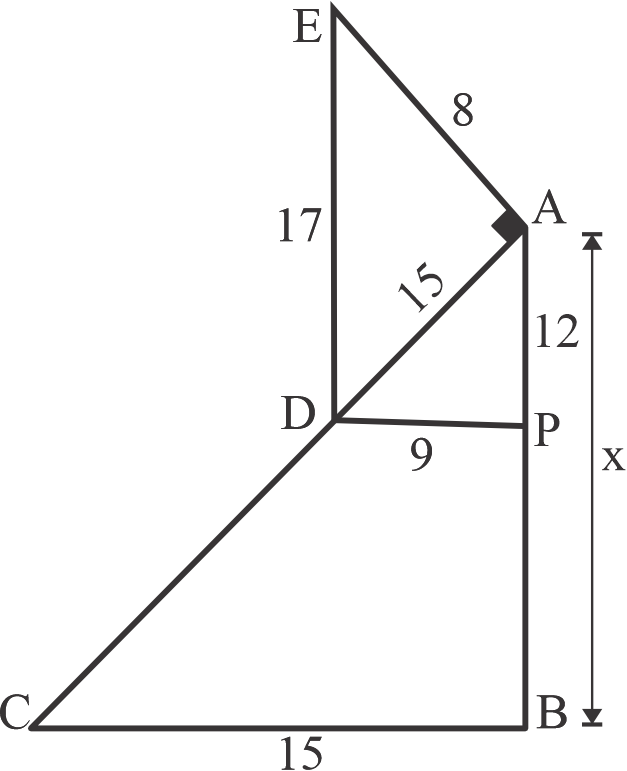
\includegraphics[width=3.8cm]{imagenes/general2024-I/etapa2/bio/geo3g24-IIr.png}
		\end{minipage}
	\end{center}
	
	\vspace{6mm}
	
	
\end{enumerate}





\subsection*{Trigonometría}

\begin{enumerate}[resume]
	
	\item En la figura, calcule ctg $\theta$
	
	\begin{center}
		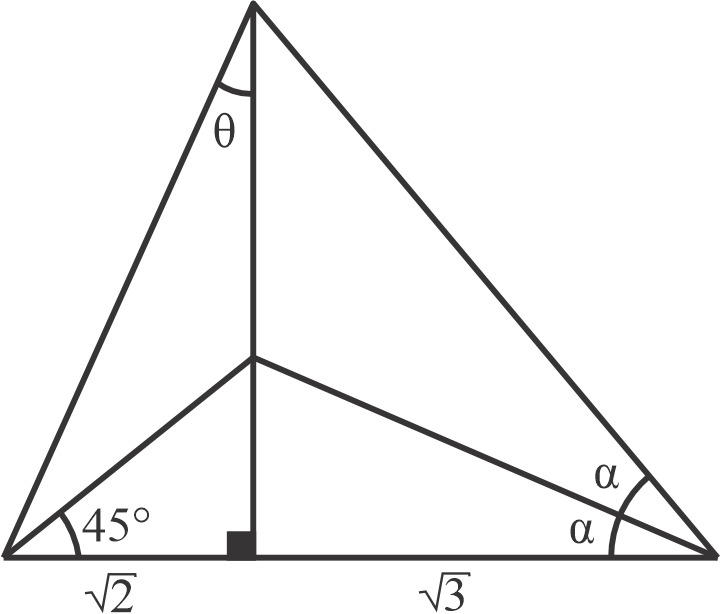
\includegraphics[width=4cm]{imagenes/general2024-I/etapa2/bio/trigo1g24-II.png}
	\end{center}
	
	\begin{enumerate}[label=\alph*)]
		\item 4
		\item $\sqrt{6}$
		\item 6
		\item 2$\sqrt{2}$
		\item 4$\sqrt{3}$
	\end{enumerate}
	\textbf{Respuesta correcta:} c)
	
	\vspace{2mm}
	\textbf{Solucionario:}
	
	$\tan \alpha = \dfrac{\sqrt{2}}{\sqrt{3}} \quad , \quad \tan 2\alpha = \dfrac{x + \sqrt{2}}{\sqrt{3}}$
	
	
	$\dfrac{2\tan \alpha}{1 - \tan^2 \alpha} = \dfrac{x + \sqrt{2}}{\sqrt{3}}$
	
	$\dfrac{\dfrac{2\sqrt{2}}{\sqrt{3}}}{1 - \dfrac{2}{3}} = \dfrac{x + \sqrt{2}}{\sqrt{3}}$
	
	$6\sqrt{2} = x + \sqrt{2}$
	
	$x = 5\sqrt{2}$
	
	$\text{ctg} \theta = \dfrac{6\sqrt{2}}{\sqrt{2}} = \fbox{6}$
	
	\vspace{6mm}
	
	\item En la figura, calcule CD
	
	\begin{center}
		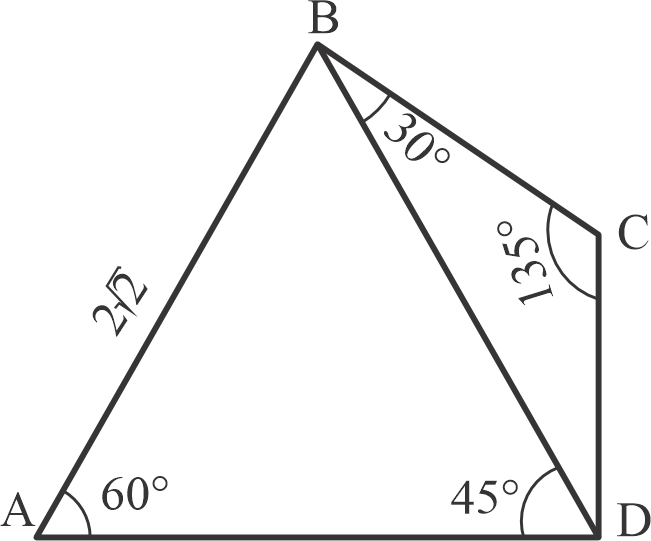
\includegraphics[width=4cm]{imagenes/general2024-I/etapa2/bio/trigo2g24-II.png}
	\end{center}
	
	\begin{enumerate}[label=\alph*)]
		\item $\sqrt{7}$
		\item $\sqrt{6}$
		\item $\sqrt{5}$
		\item $\sqrt{3}$
		\item $\sqrt{2}$
	\end{enumerate}
	\textbf{Respuesta correcta:} b)
	
	\vspace{2mm}
	\textbf{Solucionario:}
	
	\begin{center}
		\begin{minipage}{0.45\textwidth}
			
			\begin{flushright}
				ABD \qquad  | \qquad BCD\\
			\end{flushright} 
			$a = \dfrac{\text{sen}60^\circ \cdot 2\sqrt{2}}{\text{sen}45^\circ} \qquad | \qquad X = \dfrac{\text{sen}30^\circ \cdot a}{\text{sen}135^\circ}$\\
			
			De ambos\\
			
			$X = \dfrac{\text{sen}30^\circ}{\text{sen}135^\circ} \cdot \dfrac{\text{sen}60^\circ \cdot 2\sqrt{2}}{\text{sen}45^\circ}$\\
			
			\fbox{$X = \sqrt{6}$}
			
			\vspace{6mm}
		\end{minipage}
		\hfill
		\begin{minipage}{0.45\textwidth}
			\centering
			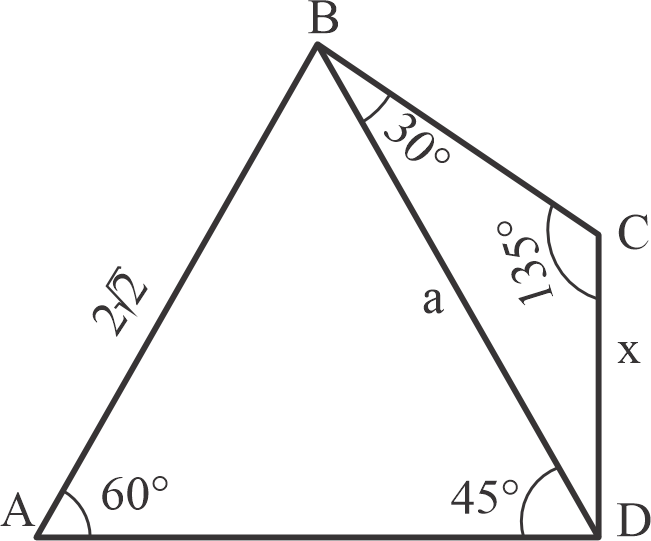
\includegraphics[width=4cm]{imagenes/general2024-I/etapa2/bio/trigo2g24-IIr.png}
		\end{minipage}
	\end{center}
	
	
	\vspace{6mm}
	
	
	\item Si $\dfrac{\csc x}{\text{sen } x} + \dfrac{\sec x}{\cos x} = n$. Calcule $\tan^2 x + \cot^2 x$
	\begin{enumerate}[label=\alph*)]
		\item $n-1$
		\item $n+2$
		\item $n-2$
		\item $n+1$
		\item $-n$
	\end{enumerate}
	\textbf{Respuesta correcta:} c)
	
	\vspace{2mm}
	\textbf{Solucionario:}\\
	
	$\dfrac{\csc x}{\text{sen } x} + \dfrac{\sec x}{\cos x} = n$
	
	$\dfrac{1}{\text{sen}^2 x} + \dfrac{1}{\cos^2 x} = n$
	
	$\dfrac{\cos^2 x + \text{sen}^2 x}{\text{sen}^2 x \cdot \cos^2 x} = n$
	
	$(\sec x \cdot \csc x)^2 = n$
	
	$(\tan x + \cot x)^2 = n$
	
	$\tan^2 x + \cot^2 x + 2 = n$
	
	$\tan^2 x + \cot^2 x = \fbox{ n - 2}$
	
	\vspace{6mm}
	
\end{enumerate}








\subsection*{Física}

\begin{enumerate}[resume]
	
	\item Ha ocurrido un accidente de tránsito y al lugar de los hechos ha llegado una ambulancia donde el personal está atendiendo a los heridos. La ambulancia estacionada tiene encendida su sirena sonora, la cual emite una potencia de $4\pi \times 10^{-2}$ W. Determine con qué nivel de intensidad percibe el sonido de la sirena una persona que se ubica a 10 m de la ambulancia.
	\begin{enumerate}[label=\alph*)]
		\item 80 dB
		\item 90 dB
		\item 70 dB
		\item 60 dB
		\item 50 dB
	\end{enumerate}
	\textbf{Respuesta correcta:} a)
	
	\vspace{2mm}
	\textbf{Solucionario:}
	
	\begin{center}
		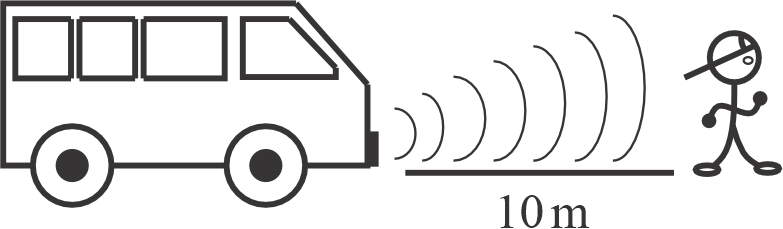
\includegraphics[width=5cm]{imagenes/general2024-I/etapa2/bio/fisica1g24-IIr.png}
	\end{center}
	
	$I = \dfrac{P}{A} = \dfrac{P}{4\pi r^2} = \dfrac{4\pi \cdot 10^{-2}}{4\pi \cdot (10)^2} = 10^{-4}$
	
	$\beta = 10 \log \left( \dfrac{I}{10^{-12}} \right) = 10 \log \left( \dfrac{10^{-4}}{10^{-12}} \right) = 10 \log (10^8)$
	
	$= (10)(8) = \fbox{80 \text{ dB}}$
	
	\vspace{6mm}
	
	\item Un recipiente que está térmicamente aislado contiene agua a 8 °C. Si se introduce 40 g de hielo (a 0 °C) y se observa que el hielo se funde en un 10\%. ¿cuántos gramos de agua había inicialmente en el recipiente? ($L_f = 80$ cal/g)
	\begin{enumerate}[label=\alph*)]
		\item 50 g
		\item 10 g
		\item 40 g
		\item 30 g
		\item 20 g
	\end{enumerate}
	\textbf{Respuesta correcta:} c)
	
	\vspace{2mm}
	\textbf{Solucionario:}
	
	$Q_{\text{g Hielo}} = -Q_{\text{perdido H}_2\text{O}}$
	
	$m_{\text{Hielo}} L_f = - c_{\text{H}_2\text{O}} m_{\text{H}_2\text{O}}  AT$
	
	
	$m_{\text{H}_2\text{O}} = - \dfrac{m_{\text{Hielo}} L_f}{c_{\text{H}_2\text{O}}  AT}$
	
	
	$m_{\text{H}_2\text{O}} = - \dfrac{(40)(10\%)(80)}{(1)(0-8)} = \dfrac{(4)(80)}{8}$
	
	
	$m_{\text{H}_2\text{O}} = \fbox{40 \text{ g}}$
	
	\vspace{6mm}
	
	\item Una esfera dieléctrica no conductora de radio $R$ se encuentra cargada uniformemente en todo su volumen con $+Q$. Determine la magnitud del campo eléctrico en un punto fuera de la esfera que está a una distancia $d$ del centro de la esfera.
	\begin{enumerate}[label=\alph*)]
		\item $\dfrac{1}{2\pi\varepsilon_0} \dfrac{Q}{d^2}$
		\item $\dfrac{1}{2\pi\varepsilon_0} \dfrac{Q}{R^2}$
		\item $\dfrac{1}{\pi\varepsilon_0} \dfrac{Q}{d^2}$
		\item $\dfrac{1}{4\pi\varepsilon_0} \dfrac{Q}{d^2}$
		\item $\dfrac{1}{4\pi\varepsilon_0} \dfrac{Q}{R^2}$
	\end{enumerate}
	\textbf{Respuesta correcta:} d)
	
	\vspace{2mm}
	\textbf{Solucionario:}
	
	$\phi = E A$
	
	$\phi = E A = \dfrac{Q}{\varepsilon_0}$
	
	$E = \dfrac{Q}{A \varepsilon_0}$\
	
	\fbox{$E = \dfrac{Q}{4\pi d^2 \varepsilon_0}$}
	
	\vspace{6mm}
	
\end{enumerate}





\subsection*{Química}

\begin{enumerate}[resume]
	
	\item ¿Cuál es la masa en gramos de una molécula de ácido nítrico ($\text{HNO}_3$)?\\
	($\text{H}=1$; $\text{N}=14$; $\text{O}=16$)
	\begin{enumerate}[label=\alph*)]
		\item $10,0 \times 10^{23}$
		\item $10,5 \times 10^{22}$
		\item $9,0 \times 10^{-22}$
		\item $10,5 \times 10^{-23}$
		\item $11,5 \times 10^{-23}$
	\end{enumerate}
	\textbf{Respuesta correcta:} d)
	
	\vspace{2mm}
	\textbf{Solucionario:}
	
	Determinando el peso molecular del $\text{HNO}_3$:
	
	\begin{itemize}
		\item $\text{H} = 1 \times 1 = 1$
		\item $\text{N} = 14 \times 1 = 14$
		\item $\text{O} = 16 \times 3 = 48$
	\end{itemize}
	Suma: $1 + 14 + 48 = 63\text{ g/mol}$
	
	Regla de tres simple:
	
	$63\text{ g} \text{ --- } 6,0 \times 10^{23} \text{ moléculas} $
	
	$ X \text{ ------ } 1 \text{ molécula} $
	
	$X = \dfrac{63}{6,0 \times 10^{23}} = 10,5 \times $ \fbox{$10^{-23} \text{ g}$} 
	
	\vspace{6mm}
	
	\item En un recipiente se tiene una mezcla de $1\text{ mol}$ de A y $1\text{ mol}$ de B; al reaccionar ambas sustancias se consumen $0,2\text{ moles}$ de A, estableciéndose el siguiente equilibrio a $400\text{ °C}$
	\[ \text{A}_{(g)} + \text{B}_{(g)} \rightleftharpoons 2\text{C}_{(g)} \]
	Calcule $K_c$.
	\begin{enumerate}[label=\alph*)]
		\item 0,40
		\item 0,25
		\item 0,30
		\item 0,20
		\item 0,35
	\end{enumerate}
	\textbf{Respuesta correcta:} b)
	
	\vspace{2mm}
	\textbf{Solucionario:}
	
	Sabiendo que:
	
	$\text{A}_{(g)} + \text{B}_{(g)} \rightleftharpoons 2\text{C}_{(g)}$
	
	se dan las siguientes relaciones:
	
	\begin{center}
		\begin{tabular}{lccc}
			& A & B & C \\
			Inicio & $1\text{ mol}$ & $1\text{ mol}  \rightleftharpoons $ & --- \\
			Avance & $0,2\text{ mol}$ & $0,2\text{ mol}  \rightleftharpoons$ & --- \\
			Equilibrio & $0,8\text{ mol}$ & $0,8\text{ mol} \rightleftharpoons$ & $2(0,2\text{ mol})$
		\end{tabular}
	\end{center}
	
	$ K_c = \dfrac{[\text{C}]^2}{[\text{A}][\text{B}]} \rightarrow K_c = \dfrac{(0,4)^2}{(0,8)(0,8)} \rightarrow$ \fbox{$K_c = 0,25 $}
	
	\vspace{6mm}
	
	\item Determine la masa de $\text{HNO}_3$ puro que está disuelto en $400\text{ cm}^3$ de una solución acuosa cuya densidad es $1,3\text{ g/cm}^3$ y contiene $30\%$ en masa de este ácido.
	\begin{enumerate}[label=\alph*)]
		\item 156
		\item 166
		\item 136
		\item 150
		\item 140
	\end{enumerate}
	\textbf{Respuesta correcta:} a)
	
	\vspace{2mm}
	\textbf{Solucionario:}

	Datos:
	
	$m = ?$
	
	$V = 400\text{ cm}^3$
	
	$\rho = 1,3\text{ g/cc}$
	
	Si $\rho = \dfrac{m}{V} \rightarrow m = \rho \cdot V$
	
	$ m = 1,3 \times 400 = 520\text{ g} $
	
	Si tiene el $30\%$ en masa:
	
	$ m = 520 \times 30\% $
	
	\fbox{$m = 156\text{ g} $}
	
	\vspace{6mm}
	
	\item Determine el número de fotones que emite durante 1 minuto de funcionamiento una linterna cuya potencia eléctrica es de 20 watts. Si emite una luz roja de $700\text{ nm}$ de longitud de onda.\\
	($1\text{ watt} = 1\text{ J/s}$; $h = 6,626 \times 10^{-34}\text{ J}\cdot\text{s}$; $1\text{ nm} = 10^{-9}\text{ m}$)
	\begin{enumerate}[label=\alph*)]
		\item $4,23 \times 10^{19}$
		\item $4,23 \times 10^{22}$
		\item $4,22 \times 10^{18}$
		\item $4,23 \times 10^{21}$
		\item $4,23 \times 10^{-19}$
	\end{enumerate}
	\textbf{Respuesta correcta:} d)
	
	\vspace{2mm}
	\textbf{Solucionario:}
	
	$E_{total} = \dfrac{20\text{ J}}{\text{s}} \times 60\text{ s} = 1200\text{ J}$
	
	Cálculo de la Energía de la luz roja ($\varepsilon$):
	
	$ \varepsilon = \dfrac{hc}{\lambda} = \dfrac{6,626 \times 10^{-34}\text{ J}\cdot\text{s} \times 3 \times 10^8\text{ m/s}}{700\text{ nm} \times \dfrac{1\text{ m}}{10^9\text{ nm}}} $
	
	$ \varepsilon = 2,84 \times 10^{-19}\text{ J} $
	
	Número de fotones ($N_{fot}$):

	$ N_{fot} = \dfrac{E_{total}}{\varepsilon} = \dfrac{1200\text{ J}}{2,84 \times 10^{-19}\text{ J}} $\\
	
	\fbox{$ N_{fot} = 4,23 \times 10^{21} $}
	
	\vspace{6mm}
	
	\item Halle el volumen de aire que se necesita para la combustión de 3 litros de acetileno ($\text{C}_2\text{H}_2$) y el volumen de dióxido de carbono ($\text{CO}_2$), según la reacción:
	\[ \text{C}_2\text{H}_2 + \text{O}_2 \rightarrow \text{CO}_2 + \text{H}_2\text{O} \]
	(Aire: $\text{O}_2 = 20\%$; $\text{N}_2 = 80\%$ en volumen)
	\begin{enumerate}[label=\alph*)]
		\item $35,7\text{ L}$ y $6\text{ L}$
		\item $3,7\text{ L}$ y $5\text{ L}$
		\item $37,5\text{ L}$ y $3\text{ L}$
		\item $7,5\text{ L}$ y $6\text{ L}$
		\item $37,5\text{ L}$ y $6\text{ L}$
	\end{enumerate}
	\textbf{Respuesta correcta:} e)
	
	\vspace{2mm}
	\textbf{Solucionario:}\\[1mm]
	Se tiene la reacción y la balanceamos:
	
	$ 1\text{C}_2\text{H}_2 + \dfrac{5}{2}\text{O}_2 \rightarrow 2\text{CO}_2 + \text{H}_2\text{O} $\\
	
	Relación de volúmenes:
	
	$ 1\text{V}_{\text{C}_2\text{H}_2} \text{ --- } \dfrac{5}{2}\text{V}_{\text{O}_2} \text{ --- } 2\text{V}_{\text{CO}_2} $
	
	$ 3\text{ L} \text{ --------- } \text{V}_{\text{O}_2} \text{ ------ } \text{V}_{\text{CO}_2} $
	
	Cálculo de $\text{V}_{\text{O}_2}$:
	
	$ \text{V}_{\text{O}_2} = \dfrac{(3\text{ L})(\dfrac{5}{2}\text{ V})}{1\text{ V}} = 7,5\text{ L} $
	Cálculo de $\text{V}_{\text{CO}_2}$:
	
	$ \text{V}_{\text{CO}_2} = \dfrac{(3\text{ L})(2\text{ V})}{1\text{ V}} = 6\text{ L} $
	Cálculo del volumen de aire:
	
	$ V_{aire} = \dfrac{\text{V}_{\text{O}_2}}{20\%} \rightarrow V_{aire} = \dfrac{7,5\text{ L}}{20\%} \rightarrow$  \fbox{$V_{aire} = 37,5\text{ L} $}
	
	\vspace{6mm}
	
\end{enumerate}






\subsection*{Biología y Anatomía}

\begin{enumerate}[resume]
	
	\item Es la cantidad de aire que permanece en los pulmones al final de una espiración normal. Su valor resulta de la suma del volumen residual más el volumen de reserva espiratorio.
	\begin{enumerate}[label=\alph*)]
		\item volumen de aire corriente (VAC)
		\item volumen de reserva inspiratoria (VRI)
		\item volumen de respiración minuto (Vm)
		\item capacidad funcional inspiratoria (CFI)
		\item capacidad funcional residual (CFR)
	\end{enumerate}
	\textbf{Respuesta correcta:} e)
	
	\vspace{2mm}
	\textbf{Solucionario:}\\[1mm]
	La Capacidad Funcional Residual (CFR) es la suma del Volumen de Reserva Espiratorio (VRE) y el Volumen Residual (VR). Representa el aire que queda en los pulmones tras una espiración pasiva.
	
	\vspace{6mm}
	
	\item ¿Cuál es el microorganismo de importancia en la industria panificadora e industria de bebidas alcohólicas?
	\begin{enumerate}[label=\alph*)]
		\item Escherichia coli
		\item Rhizobium leguminosarum
		\item Saccharomyces cerevisiae
		\item Clostridium acetobutylicum
		\item Bacillus thuringiensis
	\end{enumerate}
	\textbf{Respuesta correcta:} c)
	
	\vspace{2mm}
	\textbf{Solucionario:}\\[1mm]
	\textit{Saccharomyces cerevisiae} es una levadura unicelular fundamental en la fermentación alcohólica, proceso clave para la producción de pan, cerveza y vino.
	
	\vspace{6mm}
	
	\item Son dos masas ovoideas formadas por sustancia gris, localizadas a ambos lados del tercer ventrículo. Su función es la de servir de estación de relevo para todos los impulsos sensitivos.
	\begin{enumerate}[label=\alph*)]
		\item Aracnoides
		\item Tálamo
		\item Duramadre
		\item Hipotálamo
		\item Cerebelo
	\end{enumerate}
	\textbf{Respuesta correcta:} b)
	
	\vspace{2mm}
	\textbf{Solucionario:}\\[1mm]
	El tálamo actúa como el principal centro de relevo sensorial de la zona cerebral; procesa y transmite la información sensorial a las áreas correspondientes de la corteza cerebral (excepto el olfato).
	
	\vspace{6mm}
	
	\item Los genotipos $X^dY$ y RHrh corresponde a:
	\begin{enumerate}[label=\alph*)]
		\item varón portador, Rh (+)
		\item varón hemofílico, Rh (-)
		\item varón daltónico, Rh (+)
		\item varón daltónico, Rh (-)
		\item varón sano, Rh (+)
	\end{enumerate}
	\textbf{Respuesta correcta:} c)
	
	\vspace{2mm}
	\textbf{Solucionario:}\\[1mm]
	El genotipo $X^dY$ indica un varón que posee el gen recesivo del daltonismo en su único cromosoma X, por lo tanto es daltónico. El genotipo $RHrh$ es heterocigoto, lo que se manifiesta como fenotipo Rh positivo.
	
	\vspace{6mm}
	
	\item El hígado, considerado como "laboratorio central" del cuerpo, puede realizar más de cien funciones diferentes. Respecto a su participación en el proceso de la digestión, señale la secuencia correcta de verdadero (V) y falso (F).
	\begin{itemize}
		\item[I.] Los conductos hepático común y acino portal forman el colédoco.
		\item[II.] La función del hígado en la digestión es producir la bilis.
		\item[III.] Las sales biliares se sintetizan a partir de los fosfolípidos y aminoácidos.
		\item[IV.] La bilis es almacenada y concentrada en la vesícula biliar.
		\item[V.] La bilis emulsifica la grasa formando micelas para su absorción.
	\end{itemize}
	\begin{enumerate}[label=\alph*)]
		\item FFFVV
		\item VFFVF
		\item FVFVV
		\item VVFFF
		\item FVVFV
	\end{enumerate}
	\textbf{Respuesta correcta:} c)
	
	\vspace{2mm}
	\textbf{Solucionario:}\\[1mm]
	I(F): El colédoco se forma por la unión del conducto cístico y el hepático común.\\
	II(V): El hígado produce bilis. \\
	III(F): Se sintetizan a partir del colesterol. \\
	IV(V): La vesícula almacena la bilis. \\
	V(V): La emulsificación facilita la digestión de grasas.
	
	\vspace{6mm}
	
	\item La oxitocina es producida en el \underline{\hspace{3cm}} y almacenada en la \underline{\hspace{3cm}}.
	\begin{enumerate}[label=\alph*)]
		\item núcleo paraventricular - neurohipófisis
		\item sistema portal hipofisiario - adenohipófisis
		\item lóbulo anterior - neurohipófisis
		\item lóbulo posterior - quiasma óptica
		\item núcleo supraóptico - neurofisina
	\end{enumerate}
	\textbf{Respuesta correcta:} a)
	
	\vspace{2mm}
	\textbf{Solucionario:}\\[1mm]
	La oxitocina se sintetiza principalmente en el núcleo paraventricular del hipotálamo y se transporta para su almacenamiento y posterior liberación a la neurohipófisis (hipófisis posterior).
	
	\vspace{6mm}
	
	
	
	
	
\end{enumerate}



\subsection*{Psicología y Filosofía}

\begin{enumerate}[resume]
	
	\item Cada vez que el profesor de inglés menciona la palabra examen, Ramiro experimenta una baja en su temperatura y comienza a tiritar ante la palabra examen. La conducta de tiritar ante la palabra examen se denomina:
	\begin{enumerate}[label=\alph*)]
		\item condicionada.
		\item incondicionada.
		\item refleja.
		\item orientadora.
		\item neutral.
	\end{enumerate}
	\textbf{Respuesta correcta:} a)
	
	\vspace{2mm}
	\textbf{Solucionario:}\\[1mm]
	En el condicionamiento clásico, una respuesta que originalmente era natural (incondicionada) ante un estímulo biológico, pasa a ser una respuesta condicionada cuando es provocada por un estímulo previamente neutro (la palabra "examen") que ha sido asociado al evento original.
	
	\vspace{6mm}
	
	\item Un taxista dice que las mujeres deberían estar cocinando y no conduciendo. Esta manera de pensar se denomina:
	\begin{enumerate}[label=\alph*)]
		\item discriminación.
		\item actitud.
		\item prejuicio.
		\item aprendizaje.
		\item estereotipo.
	\end{enumerate}
	\textbf{Respuesta correcta:} c)
	
	\vspace{2mm}
	\textbf{Solucionario:}\\[1mm]
	El prejuicio es una actitud preconcebida, generalmente negativa, hacia los miembros de un grupo social. En este caso, el juicio de valor sobre lo que "deberían" hacer las mujeres refleja una predisposición afectiva y cognitiva antes de conocer la capacidad individual de la persona.
	
	\vspace{6mm}
	
	\item Para los estoicos, ¿Cuándo uno es feliz?
	\begin{enumerate}[label=\alph*)]
		\item Cuando se practica la prudencia.
		\item Cuando se logra la autarquía.
		\item Cuando se acepta lo que se es.
		\item Cuando se logra tener placer.
		\item Cuando se hace lo que conviene a la mayoría.
	\end{enumerate}
	\textbf{Respuesta correcta:} c)
	
	\vspace{2mm}
	\textbf{Solucionario:}\\[1mm]
	La ética estoica propone que la felicidad se alcanza a través de la "apatheia" y la aceptación del orden racional del universo. Aceptar lo que uno es y lo que le acontece (el destino) permite vivir en armonía con la naturaleza y alcanzar la tranquilidad del alma.
	
	\vspace{6mm}
	
	\item Los nativos de África tienen una forma de valorar la belleza que difiere de los nativos de las tribus sudamericanas, esto sería una idea que apoyaría la teoría de:
	\begin{enumerate}[label=\alph*)]
		\item Sócrates
		\item Protágoras
		\item Demócrito
		\item Anaxágoras
		\item Heráclito
	\end{enumerate}
	\textbf{Respuesta correcta:} b)
	
	\vspace{2mm}
	\textbf{Solucionario:}\\[1mm]
	Protágoras, con su máxima "el hombre es la medida de todas las cosas", sostiene el relativismo. Esto implica que valores como la belleza no son universales, sino que dependen de la percepción de cada individuo o cultura.
	
	\vspace{6mm}
	
\end{enumerate}


\subsection*{Geografía}

\begin{enumerate}[resume]
	
	\item La consecuencia del movimiento de rotación de la Tierra es la sucesión del día y la noche. Entonces, por regla general, ...
	\begin{enumerate}[label=\alph*)]
		\item en todo lugar que se localiza al oeste de otro amanece primero
		\item en todo lugar que se localiza al este de otro amanece primero
		\item en todo lugar que se localiza al norte de otro amanece primero
		\item en todo lugar que se localiza al sur de otro amanece primero
		\item en todo lugar que se localiza delante de otro amanece primero
	\end{enumerate}
	\textbf{Respuesta correcta:} b)
	
	\vspace{2mm}
	\textbf{Solucionario:}\\[1mm]
	Debido a que la Tierra rota de oeste a este, los lugares situados más hacia el oriente (este) visualizan el sol antes que los lugares al occidente. Por lo tanto, el amanecer ocurre primero en las zonas orientales.
	
	\vspace{6mm}
	
	\item La biodiversidad es la variabilidad de los organismos vivos por:
	\begin{enumerate}[label=\alph*)]
		\item ecosistemas.
		\item especies.
		\item recursos naturales.
		\item unidad de superficie.
		\item afinidad biológica.
	\end{enumerate}
	\textbf{Respuesta correcta:} d)
	
	\vspace{2mm}
	\textbf{Solucionario:}\\[1mm]
	En ciertos contextos de análisis geográfico y ecológico, la biodiversidad se cuantifica y evalúa como la variabilidad o riqueza de especies y ecosistemas presentes en una unidad de superficie determinada, permitiendo comparar la densidad biológica entre distintas regiones.
	
	\vspace{6mm}
	
\end{enumerate}


\subsection*{Historia}

\begin{enumerate}[resume]
	
	\item Las investigaciones de Louis Pasteur (1822 - 1895) sobre la fermentación permitió el desarrollo de la:
	\begin{enumerate}[label=\alph*)]
		\item fitología.
		\item microbiología.
		\item virología.
		\item ficología.
		\item micología.
	\end{enumerate}
	\textbf{Respuesta correcta:} b)
	
	\vspace{2mm}
	\textbf{Solucionario:}\\[1mm]
	Louis Pasteur demostró que los procesos de fermentación y enfermedades infecciosas son causados por microorganismos, lo que dio inicio a la microbiología como ciencia médica y biológica.
	
	\vspace{6mm}
	
	\item El Hospital Naval, el Hospital Militar y el Hospital Central del Empleado en Lima, así como los hospitales regionales en los departamentos, fueron construidos durante el gobierno del Presidente:
	\begin{enumerate}[label=\alph*)]
		\item Manuel A. Odría.
		\item Manuel Prado Ugarteche.
		\item José Luis Bustamante y Rivero.
		\item Ricardo Pérez Godoy.
		\item Augusto B. Leguía.
	\end{enumerate}
	\textbf{Respuesta correcta:} a)
	
	\vspace{2mm}
	\textbf{Solucionario:}\\[1mm]
	El gobierno de Manuel A. Odría (1948-1956) se caracterizó por una fuerte inversión en salud y educación, construyendo las Grandes Unidades Escolares y los principales centros hospitalarios de la capital y provincias.
	
	\vspace{6mm}
	
\end{enumerate}

\subsection*{Educación Cívica}

\begin{enumerate}[resume]
	
	\item La \underline{\hspace{3cm}} es un organismo cuyo propósito es mejorar a través de la acción internacional las condiciones de trabajo y los niveles de vida, promoviendo la estabilidad social y económica.
	\begin{enumerate}[label=\alph*)]
		\item OMS
		\item OMC
		\item OIT
		\item UNESCO
		\item UNICEF
	\end{enumerate}
	\textbf{Respuesta correcta:} c)
	
	\vspace{2mm}
	\textbf{Solucionario:}\\[1mm]
	La Organización Internacional del Trabajo (OIT) es el organismo especializado de la ONU que se ocupa de los asuntos relativos al trabajo y las relaciones laborales a nivel mundial.
	
	\vspace{6mm}
	
	\item Una de las atribuciones del Congreso de la República del Perú, de acuerdo a la Constitución, es:
	\begin{enumerate}[label=\alph*)]
		\item conceder indultos y conmutar penas.
		\item convocar a elecciones generales, parlamentarias, regionales y locales.
		\item aprobar el presupuesto y la Cuenta General de la República.
		\item velar por el orden interno y externo.
		\item dirigir la política general del Gobierno.
	\end{enumerate}
	\textbf{Respuesta correcta:} c)
	
	\vspace{2mm}
	\textbf{Solucionario:}\\[1mm]
	Dentro de la función legislativa y de control, el Congreso tiene la facultad exclusiva de aprobar el presupuesto público propuesto por el Ejecutivo y revisar la ejecución del mismo a través de la Cuenta General.
	
	\vspace{6mm}
	
\end{enumerate}


\subsection*{Economía}

\begin{enumerate}[resume]
	
	\item La palta, conocida también como "oro verde", ocupó en los últimos años los primeros lugares en exportación del grupo de los productos agroindustriales. Según el BCRP, el producto señalado es considerado de exportación:
	\begin{enumerate}[label=\alph*)]
		\item no tradicional.
		\item temporal.
		\item tradicional.
		\item definitiva.
		\item sin valor comercial.
	\end{enumerate}
	\textbf{Respuesta correcta:} a)
	
	\vspace{2mm}
	\textbf{Solucionario:}\\[1mm]
	Las exportaciones no tradicionales son productos que tienen un mayor valor agregado o que históricamente no eran el fuerte de la balanza comercial. La palta pertenece al sector agroindustrial, el cual es un eje clave de las exportaciones no tradicionales en el Perú.
	
	\vspace{6mm}
	
	\item El incremento del precio de los insumos para la elaboración de un bien en un mercado de competencia perfecta genera:
	\begin{enumerate}[label=\alph*)]
		\item un aumento de la demanda.
		\item un aumento de las ganancias del vendedor.
		\item un incremento de la cantidad ofertada.
		\item una expansión de la oferta.
		\item una contracción de la oferta.
	\end{enumerate}
	\textbf{Respuesta correcta:} e)
	
	\vspace{2mm}
	\textbf{Solucionario:}\\[1mm]
	Cuando los costos de producción aumentan (debido al alza de precio de los insumos), producir el mismo bien resulta más caro. Esto provoca que los productores estén dispuestos a ofrecer menos cantidad al mismo precio, lo que se traduce gráficamente como un desplazamiento de la curva de oferta hacia la izquierda (contracción).
	
	\vspace{6mm}
	
\end{enumerate}

\subsection*{Comunicación}

\begin{enumerate}[resume]
	
	\item La tuberculosis es una enfermedad pulmonar contagiosa que se transmite por el aire. \\ ¿A qué tipo de texto corresponde?
	\begin{enumerate}[label=\alph*)]
		\item Narrativo
		\item Expositivo
		\item Instructivo
		\item Argumentativo
		\item Descriptivo
	\end{enumerate}
	\textbf{Respuesta correcta:} b)
	
	\vspace{2mm}
	\textbf{Solucionario:}\\[1mm]
	El texto presenta información objetiva y conceptos sobre una realidad específica (la tuberculosis) con el fin de informar al receptor, característica principal de los textos expositivos.
	
	\vspace{6mm}
	
	\item Consiste en expresar de manera condensada y coherente el contexto esencial del texto. Se realiza a partir de la síntesis global del contenido. \\ ¿A qué tipo de técnica de estudio corresponde?
	\begin{enumerate}[label=\alph*)]
		\item Subrayado
		\item Esquema
		\item Notas al margen
		\item Secuencia
		\item Resumen
	\end{enumerate}
	\textbf{Respuesta correcta:} e)
	
	\vspace{2mm}
	\textbf{Solucionario:}\\[1mm]
	El resumen es la técnica de estudio que reduce un texto a sus ideas fundamentales, manteniendo la coherencia y la esencia del mensaje original pero de forma abreviada.
	
	\vspace{6mm}
	
	\item Es una forma de interacción comunicativa oral y planificada, en la que distintos interlocutores asumen posturas contrarias a partir de un tema polémico.
	\begin{enumerate}[label=\alph*)]
		\item Seminario
		\item Debate
		\item Informe oral
		\item Entrevista
		\item Plenario
	\end{enumerate}
	\textbf{Respuesta correcta:} b)
	
	\vspace{2mm}
	\textbf{Solucionario:}\\[1mm]
	El debate es una técnica de comunicación que consiste en la confrontación de ideas u opiniones diferentes sobre un tema determinado, donde los participantes defienden sus posturas con argumentos.
	
	\vspace{6mm}
	
	\item El \underline{\hspace{3cm}} es un organizador gráfico que resume un texto de manera organizada, jerarquizada y conectada, a través de líneas y palabras de enlace.
	\begin{enumerate}[label=\alph*)]
		\item diagrama de Ishikawa
		\item mapa mental
		\item mapa conceptual
		\item mapa semántico
		\item cuadro sinóptico
	\end{enumerate}
	\textbf{Respuesta correcta:} c)
	
	\vspace{2mm}
	\textbf{Solucionario:}\\[1mm]
	El mapa conceptual se caracteriza específicamente por el uso de conceptos encerrados en elipses o cuadros (nodos) que se relacionan entre sí mediante líneas y palabras de enlace, siguiendo una estructura jerárquica.
	
	\vspace{6mm}
	
\end{enumerate}


\subsection*{Literatura}

\begin{enumerate}[resume]
	
	\item Los poetas populares del incanato se denominaban:
	\begin{enumerate}[label=\alph*)]
		\item amautas.
		\item haravicus.
		\item purej.
		\item quipucamayoc.
		\item tucuy-ricuy.
	\end{enumerate}
	\textbf{Respuesta correcta:} b)
	
	\vspace{2mm}
	\textbf{Solucionario:}\\[1mm]
	En el Imperio Incaico, los haravicus eran los poetas populares que expresaban los sentimientos de la comunidad (amor, agro, guerra) a través de la lírica, a diferencia de los amautas, que eran los maestros y encargados de la educación formal de la nobleza.
	
	\vspace{6mm}
	
	\item "Soy cantor de América, autóctono y salvaje mi lira tiene un alma, mi canto un ideal. Mi verso no se mece colgado de un ramaje con un vaivén pausado de hamaca tropical" \\ \\ Estos versos pertenecen a:
	\begin{enumerate}[label=\alph*)]
		\item Dante Nava.
		\item Abraham Valdelomar.
		\item Ciro Alegría.
		\item José Santos Chocano.
		\item Arturo Peralta.
	\end{enumerate}
	\textbf{Respuesta correcta:} d)
	
	\vspace{2mm}
	\textbf{Solucionario:}\\[1mm]
	Estos versos corresponden al poema "Blasón", perteneciente al libro \textit{Alma América} de José Santos Chocano. Es el máximo representante del Modernismo en el Perú y se autodenominó "El Cantor de América".
	
	\vspace{6mm}
	
\end{enumerate}



\subsection*{Razonamiento Matemático}

\begin{enumerate}[resume]
	
	\item De cuántas formas se puede leer la palabra UNAP?
	
	\begin{center}
		\begin{tabular}{cccc}
			U & N & A & P \\
			N & A & P & A \\
			A & P & A & N \\
			P & A & N & U \\
		\end{tabular}
	\end{center}
	\begin{enumerate}[label=\alph*)]
		\item 32
		\item 16
		\item 20
		\item 18
		\item 24
	\end{enumerate}
	\textbf{Respuesta correcta:} b)
	
	\vspace{2mm}
	\textbf{Solucionario:}
	
	Identificamos la forma triangular que se presenta en el arreglo.
	
	
	\begin{center}
		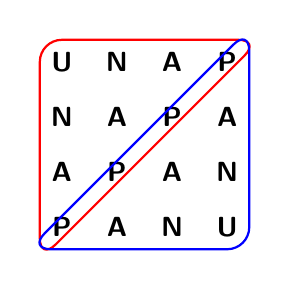
\begin{tikzpicture}[scale=0.7, every node/.style={font=\sffamily\bfseries}]
			% Matriz de letras (Arreglo de la palabra UNAP)
			\node (u1) at (0,3) {U}; \node at (1,3) {N}; \node at (2,3) {A}; \node (p1) at (3,3) {P};
			\node at (0,2) {N}; \node at (1,2) {A}; \node (p2) at (2,2) {P}; \node at (3,2) {A};
			\node at (0,1) {A}; \node (p3) at (1,1) {P}; \node at (2,1) {A}; \node at (3,1) {N};
			\node (p4) at (0,0) {P}; \node at (1,0) {A}; \node at (2,0) {N}; \node (u2) at (3,0) {U};
			
			% CUADRO ROJO (Triángulo superior izquierdo)
			% Alineado para envolver desde U (0,3) hasta la diagonal de Ps
			\draw[red, thick, rounded corners=8pt] 
			(-0.4, 3.4) -- (3.6, 3.4) -- (-0.4, -0.6) -- cycle;
			
			% CUADRO AZUL (Triángulo inferior derecho)
			% Alineado para envolver desde U (3,0) hasta la diagonal de Ps
			\draw[blue, thick, rounded corners=8pt] 
			(3.4, -0.4) -- (-0.6, -0.4) -- (3.4, 3.6) -- cycle;
			
		\end{tikzpicture}
	\end{center}
	
	\begin{itemize}
		\item UNAP 4 Letras
		\item $2^{n-1} = 2^{4-1} = 2^{3} = 8$
		\item 8 Formas
	\end{itemize}
	
	Se observa 2 veces la forma triangular
	
	$8 + 8 =$\fbox{$ 16$} Formas
	
	\vspace{6mm}
	
	
	
	
	
	
	
	
	
	\item Halle el área de la región sombreada si el lado del cuadrado $ABCD$ es $4u$.
	
	\begin{center}
		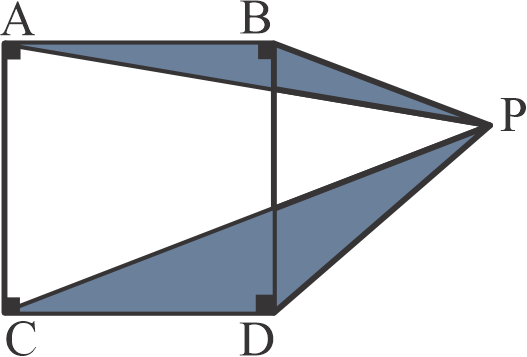
\includegraphics[width=4.4cm]{imagenes/general2024-I/etapa2/bio/rm2g24-II.png}
	\end{center}
	
	\begin{enumerate}[label=\alph*)]
		\item $5u^2$
		\item $16u^2$
		\item $12u^2$
		\item $8^2$
		\item $4u^2$
	\end{enumerate}
	\textbf{Respuesta correcta:}d)
	
	\vspace{2mm}
	\textbf{Solucionario:}
	
	\begin{center}
		\begin{minipage}{0.45\textwidth}
			
			$H1 + H2 = 4$\\
			
			$A_s = A_{s1} + A_{s2} = \dfrac{4 \cdot H1}{2} + \dfrac{4 \cdot H2}{2}$ \\
			
			$A_s = 2 H1 + 2 H2$ \\
			
			$A_s = 2 (H1 + H2)$ \\
			
			$A_s = 2 (4)$ \\
			
			\fbox{$A_s = 8$}
			
			\vspace{6mm}
		\end{minipage}
		\hfill
		\begin{minipage}{0.45\textwidth}
			\centering
			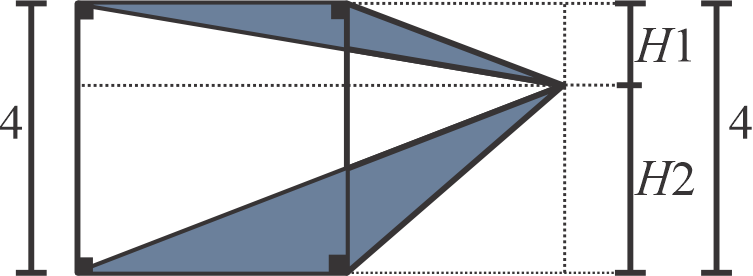
\includegraphics[width=5.4cm]{imagenes/general2024-I/etapa2/bio/rm2g24-IIr.png}
		\end{minipage}
	\end{center}
	
	
	
	
	\item Pablito le dice a José: "La suma de nuestras edades es 46 años y tu edad es el triple de la edad que tenías cuando yo tenía el triple de la edad que tuviste cuando yo nací". ¿Qué edad tiene José?
	
	\begin{enumerate}[label=\alph*)]
		\item 28
		\item 40
		\item 18
		\item 8
		\item 24
	\end{enumerate}
	\textbf{Respuesta correcta:} e)
	
	\vspace{2mm}
	\textbf{Solucionario:}
	
	
	
	\begin{center}
		
		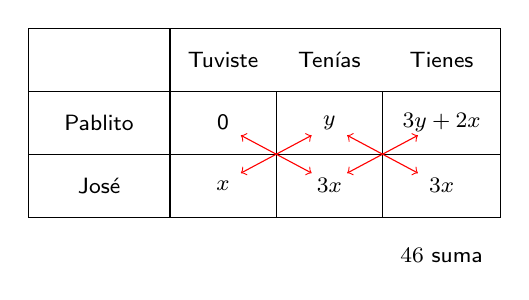
\begin{tikzpicture}[x=1.5cm, y=0.8cm, every node/.style={font=\footnotesize\sffamily}]
			% Líneas del cuadro
			\draw (0,0) rectangle (4,3);
			\draw (0,1) -- (4,1);
			\draw (0,2) -- (4,2);
			\draw (1.2,0) -- (1.2,3);
			\draw (2.1,0) -- (2.1,2);
			\draw (3,0) -- (3,2);
			
			% Encabezados
			
			\node at (1.65,2.5) {Tuviste};
			\node at (2.55,2.5) {Tenías};
			\node at (3.5,2.5) {Tienes};
			
			% Filas
			\node at (0.6,1.5) {Pablito};
			\node at (1.65,1.5) {0};
			\node at (2.55,1.5) {$y$};
			\node at (3.5,1.5) {$3y+2x$};
			
			\node at (0.6,0.5) {José};
			\node at (1.65,0.5) {$x$};
			\node at (2.55,0.5) {$3x$};
			\node at (3.5,0.5) {$3x$};
			\node at (3.5,-0.6) {$46$ suma};
			% Flechas de suma en aspa (opcionales según imagen)
			\draw[red, <->] (1.8,1.3) -- (2.4,0.7);
			\draw[red, <->] (1.8,0.7) -- (2.4,1.3);
			\draw[red, <->] (2.7,1.3) -- (3.3,0.7);
			\draw[red, <->] (2.7,0.7) -- (3.3,1.3);
		\end{tikzpicture}
		
		
		
		
	\end{center}
	
	
	
	
	Aplicamos la suma en aspa:
	
	$0 + 3x = y + 3y \Rightarrow x = 4y$ .....(I) 
	
	Planteando la primera afirmación:
	
	$(3y + 2x) + 3x = 46$ .....(II)
	
	$3y + 5x = 46$ 
	
	(I) en (II): 
	
	$3y + 5(4y) = 46 \Rightarrow y = 2 \Rightarrow x = 8$ 
	
	$\therefore$ José tiene $3(8) = 24$ años.
	
	\vspace{4mm}
	\fbox{José tiene 24 años}
	
	
	
	
	
	
	\item Se tiene un número impar, se le añade el par de números impares que le anteceden y los tres números pares que son inmediatamente anteriores a dicho número, dando un resultado de 939 unidades. Halle la suma de cifras del número impar mencionado.
	
	\begin{enumerate}[label=\alph*)]
		\item 15
		\item 16
		\item 13
		\item 19
		\item 26
	\end{enumerate}
	\textbf{Respuesta correcta: a)}
	
	\vspace{2mm}
	\textbf{Solucionario:}
	
	Suma de cifras del número impar mencionado:
	
	$\qquad\underbrace{2x+1}_{} \quad \quad +\qquad \underbrace{(2x-1), (2x-3)}_{} +\quad \underbrace{2x, 2x-2, 2x-4}_{} = 939$
	
	$\Rightarrow \left( \text{número impar} \right) + \left( \begin{tabular}{c} 2 números \\ impares que \\ anteceden \end{tabular} \right) + \left( \begin{tabular}{c} 3 números \\ pares que \\ anteceden \end{tabular} \right) = 939$
	
	
	\vspace{2mm}
	Sumando:
	
	$12x - 9 = 939$ 
	
	$x = 79$
	
	
	Número impar $= 2x + 1 = 2(79) + 1 = 159$
	
	Suma de cifras: $1 + 5 + 9 = $\fbox{15}
	
	
	\item ¿Cuántas diagonales hay en la figura?
	
	\begin{center}
		
\includegraphics[width=3cm]{imagenes/general2024-I/etapa2/bio/rm5g24-II.png}
	\end{center}
	
	
	\begin{enumerate}[label=\alph*)]
		\item 24
		\item 20
		\item 22
		\item 24
		\item 26
	\end{enumerate}
	\textbf{Respuesta correcta:} c)
	
	\vspace{2mm}
	\textbf{Solucionario:}
	
	Como cada cuadrilátero tiene dos diagonales, entonces, el número de diagonales será el doble del número de cuadriláteros:
	
	
	
	
	\begin{center}
		\begin{minipage}{0.45\textwidth}
			
			\begin{itemize}
				\item 3 cuadriláteros ($a, d, e$)
				\item 5 cuadriláteros 
				
				($ad, de, ec, bc, ab$)
				\item 2 cuadriláteros ($abc, bce$)
				\item 1 cuadrilátero ($abcde$)
			\end{itemize}
			Total: 11 cuadriláteros.\\
			
			\fbox{$\therefore$ Hay 22 diagonales.}
			
			
			\vspace{6mm}
		\end{minipage}
		\hfill
		\begin{minipage}{0.45\textwidth}
			\centering
			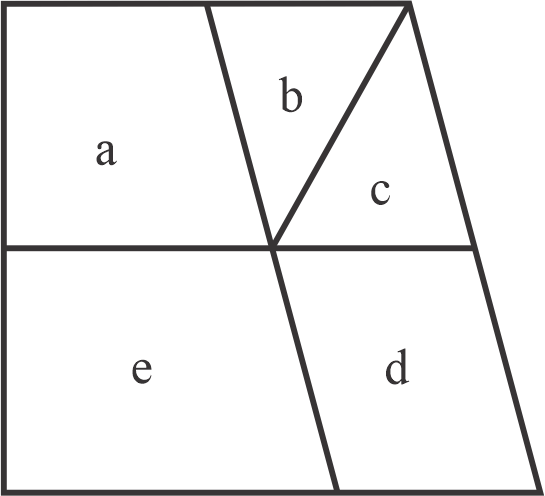
\includegraphics[width=3cm]{imagenes/general2024-I/etapa2/bio/rm5g24-IIr.png}
		\end{minipage}
	\end{center}
	
	\vspace{6mm}
	
	
	
	\item Un total de 45 estrechadas de mano se efectuaron al final de una reunión, suponiendo que cada uno de los participantes es cortés con cada uno de los demás. Determine el número de personas participantes de la reunión.
	\begin{enumerate}[label=\alph*)]
		\item 8
		\item 9
		\item 11
		\item 10
		\item 12
	\end{enumerate}
	\textbf{Respuesta correcta:} d)
	
	\vspace{2mm}
	\textbf{Solucionario:}
	
	$n$: número de personas participantes. El saludo es de dos en dos (combinatoria).
	
	$ C_{2}^{n} = \dfrac{n!}{(n-2)! 2!} = \dfrac{n(n-1)(n-2)!}{2 \times 1 \times (n-2)!} = \dfrac{n(n-1)}{2} $
	
	$ 45 = \dfrac{n(n-1)}{2} $
	
	$ 90 = n(n-1) = 10(9) $
	
	$\therefore  \fbox{n = 10}$
	
	\vspace{6mm}
	
	
	
\end{enumerate}









\subsection*{Razonamiento Verbal}

\begin{enumerate}[resume]
	
	\item Identifique el par analógico\\
	INSPIRACIÓN : PULMONES ::
	\begin{enumerate}[label=\alph*)]
		\item circulación : corazón.
		\item ingestión : estómago.
		\item segregación : páncreas.
		\item asimilación : cerebro.
		\item inoculación : vacuna.
	\end{enumerate}
	\textbf{Respuesta correcta:} b)
	
	\vspace{2mm}
	\textbf{Solucionario:}\\[1mm]
	La relación es de función-órgano: la inspiración es el proceso principal de ingreso que se realiza en los pulmones, así como la ingestión es el proceso de ingreso de alimento que se realiza en el estómago.
	
	\vspace{6mm}
	
	\item Su exposición solo fue una narrativa sin evidencia empírica. El sinónimo de la palabra NARRATIVA es:
	\begin{enumerate}[label=\alph*)]
		\item sustento.
		\item razón.
		\item prosa.
		\item motivo.
		\item pilar.
	\end{enumerate}
	\textbf{Respuesta correcta:} c)
	
	\vspace{2mm}
	\textbf{Solucionario:}\\[1mm]
	En el contexto literario y lingüístico, la narrativa está asociada formalmente a la prosa (forma de expresión habitual no sujeta a medida), a diferencia de otros términos que implican fundamentación lógica.
	
	\vspace{6mm}
	
	\item Complete la Oración\\
	La \underline{\hspace{2cm}} puede ser definida como una capa delgada de tejido animal que envuelve algún órgano o separa dos \underline{\hspace{2cm}}.
	\begin{enumerate}[label=\alph*)]
		\item piel - cuerpos
		\item célula - zonas
		\item histología - órganos
		\item membrana - cavidades
		\item epidermis - miembros
	\end{enumerate}
	\textbf{Respuesta correcta:} d)
	
	\vspace{2mm}
	\textbf{Solucionario:}\\[1mm]
	La definición técnica de membrana en anatomía es precisamente una capa delgada de tejido que tiene como función recubrir órganos o delimitar cavidades internas.
	
	\vspace{6mm}
	
	\item El término excluido de CONGÉNITO es:
	\begin{enumerate}[label=\alph*)]
		\item ínsito.
		\item ingénito.
		\item innato.
		\item ignoto.
		\item connatural.
	\end{enumerate}
	\textbf{Respuesta correcta:} d)
	
	\vspace{2mm}
	\textbf{Solucionario:}\\[1mm]
	Congénito se refiere a algo nacido con el individuo. Ínsito, ingénito, innato y connatural son sinónimos. "Ignoto" significa desconocido o no descubierto, por lo que sale del campo semántico.
	
	\vspace{6mm}
	
	\item \textbf{PLAN DE REDACCIÓN}\\
	\textbf{La Quimioterapia}
	\begin{itemize}
		\item[I.] La utilización del mercurio para combatir la sífilis constituyó un caso de aplicación temprana de la quimioterapia.
		\item[II.] La quimioterapia se concibe como el tratamiento a base de sustancias químicas que actúan en forma selectiva contra los bacilos causantes de enfermedades.
		\item[III.] En la actualidad, se vienen utilizando diversos agentes quimioterapéuticos para combatir un gran número de afecciones.
		\item[IV.] Del mismo modo, el uso de la quinina para trabajar el paludismo constituye otro caso de aplicación de la quimioterapia.
		\item[V.] Tras el éxito logrado en muchas enfermedades con la quimioterapia, es de esperar que se la emplee para tratar el cáncer.
	\end{itemize}
	\begin{enumerate}[label=\alph*)]
		\item II - I - IV - III - V
		\item II - I - IV - V - III
		\item II - IV - I - V - III
		\item III - IV - V - II - I
		\item I - IV - II - III - V
	\end{enumerate}
	\textbf{Respuesta correcta:} a)
	
	\vspace{2mm}
	\textbf{Solucionario:}\\[1mm]
	El orden lógico es: Definición (II), antecedentes históricos iniciales (I), otro caso histórico similar (IV), uso general actual (III) y perspectiva futura/específica (V).
	
	\vspace{6mm}
	
	\item \textbf{TEXTO}\\
	En Estados Unidos, hace años se detectaba un solo caso de cáncer de piel por cada mil quinientos habitantes. Antes, la gente relacionaba la piel bronceada con una apariencia más elegante y presumía sus andanzas por los balnearios y las playas. Todo esto cambió. En lugar de tenderse en la playa, uno debe buscar un lugar sombreado, adonde los rayos del sol lleguen de manera indirecta. Además, conviene utilizar cremas protectoras, según lo sugiere el Instituto del Cáncer de Estados Unidos. \\
	El tema central del texto es:
	\begin{enumerate}[label=\alph*)]
		\item El índice de cáncer a la piel en Estados Unidos.
		\item La prevención del cáncer a la piel en Estados Unidos.
		\item El cáncer a la piel un estudio estadístico.
		\item El carácter dañino de los días soleados.
		\item El cáncer y su proliferación en Norteamérica.
	\end{enumerate}
	\textbf{Respuesta correcta:} b)
	
	\vspace{2mm}
	\textbf{Solucionario:}\\[1mm]
	Aunque el texto menciona estadísticas, el núcleo de la información se centra en el cambio de hábitos (buscar sombra, uso de cremas) para evitar la enfermedad, es decir, en la prevención.
	
	\vspace{6mm}
	
\end{enumerate}

\subsection*{Inglés}

\begin{enumerate}[resume]
	
	\item Complete the sentence: \\
	A: Ana, I am worried, since yesterday I have pain in my hip. \\
	B: I'm sorry to hear that. You \underline{\hspace{2cm}} go to the doctor.
	\begin{enumerate}[label=\alph*)]
		\item should
		\item don't should
		\item are
		\item will
		\item does
	\end{enumerate}
	\textbf{Respuesta correcta:} a)
	
	\vspace{2mm}
	\textbf{Solucionario:}\\[1mm]
	El verbo modal "should" se utiliza para dar consejos o sugerencias. En este contexto, la persona B recomienda a Ana visitar al médico debido a su dolor.
	
	\vspace{6mm}
	
	\item What is the antonym of "happy"?
	\begin{enumerate}[label=\alph*)]
		\item nice
		\item beauty
		\item bad
		\item sad
		\item wonderful
	\end{enumerate}
	\textbf{Respuesta correcta:} d)
	
	\vspace{2mm}
	\textbf{Solucionario:}\\[1mm]
	El antónimo es la palabra que expresa un significado opuesto. El opuesto de estar feliz ("happy") es estar triste ("sad").
	
	\vspace{6mm}
	
\end{enumerate}

\subsection*{Quechua y Aimara}

\begin{enumerate}[resume]
	
	\item ¿Imawantaq q'apaykunatari muskhinchik? / ¿kunampisa thujsanaka mukt'aña?
	\begin{enumerate}[label=\alph*)]
		\item Ñawiwan / Nayrampi
		\item Umawan / P'iqimpi
		\item Sinqawan / Nasampi
		\item Qalluwan / Laxrampi
		\item Sunquwan / Lluqumpi
	\end{enumerate}
	\textbf{Respuesta correcta:} c)
	
	\vspace{2mm}
	\textbf{Solucionario:}\\[1mm]
	La pregunta indaga por el órgano con el que percibimos los olores (olfato). En quechua es "sinqa" (nariz) y en aimara es "nasa".
	
	\vspace{6mm}
	
	\item Wawakuna unquqtinri, ¿Maymantaq apanachik? / Wawanaka usuntapxi ukjaxa, ¿Kawkirusa aptana?
	\begin{enumerate}[label=\alph*)]
		\item Yachay wasiman / Yatina utaru
		\item Pukllana wasiman / Anataña utaru
		\item Hampina wasiman / Qullana utaru
		\item Hisp'ana wasiman / Jarisiña utaru
		\item Puñuna wasiman / Ikiña utaru
	\end{enumerate}
	\textbf{Respuesta correcta:} c)
	
	\vspace{2mm}
	\textbf{Solucionario:}\\[1mm]
	La pregunta plantea a dónde se debe llevar a los niños cuando se enferman. La respuesta lógica es al centro de salud o lugar de curación ("hampina wasi" en quechua / "qullana uta" en aimara).
	
	\vspace{6mm}
	
\end{enumerate}














\section*{Área: Sociales}

\addcontentsline{toc}{subsection}{Área: Sociales}



\subsection*{Aritmética}

\begin{enumerate}
	
	
	
	%------------------- PREGUNTA 1 -------------------
	\item En una ciudad, a la cuarta parte de la población no le gusta la natación ni futbol,
	a la mitad le gusta natación y a los cinco doceavos les gusta futbol.
	¿Qué fracción de la población gusta de la natación y el futbol?
	
	\begin{enumerate}[label=\alph*)]
		\item $\dfrac{1}{3}$
		\item $\dfrac{1}{4}$
		\item $\dfrac{1}{6}$
		\item $\dfrac{1}{2}$
		\item $\dfrac{3}{4}$
	\end{enumerate}
	
	\textbf{Respuesta correcta:} c)
	
	\vspace{2mm}
	\textbf{Solucionario:}
	
	Sea $x$ parte de la población que guste del futbol y la natación.
	
	$\left\{\dfrac{P}{4}+\dfrac{5P}{12}+\dfrac{P}{2}-x=P\right.$
	
	$\left\{\left(\dfrac{P}{4}+\dfrac{5P}{12}\right)+\dfrac{P}{2}-P=x\right.$
	
	$\dfrac{P}{6}=x$
	
	$\therefore\ \text{La fracción de la población $P$ es } $\fbox{$\dfrac{1}{6}.$}
	
	%------------------- PREGUNTA 2 -------------------
	\item 5 hornos consumen 30 toneladas de carbón en 20 días.
	¿Cuánto consumirán en 25 días 3 hornos más?
	
	\begin{enumerate}[label=\alph*)]
		\item 40 toneladas
		\item 70 toneladas
		\item 80 toneladas
		\item 60 toneladas
		\item 50 toneladas
	\end{enumerate}
	
	\textbf{Respuesta correcta:} d)
	
	\vspace{2mm}
	\textbf{Solucionario:}

	\begin{center}
		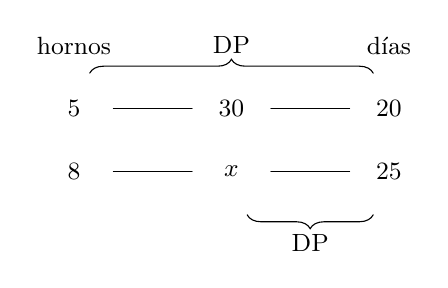
\begin{tikzpicture}[font=\small, line cap=round]
			% Títulos
			\node at (0,0.6) {hornos};
			\node at (4,0.6) {días};
			
			% Fila 1
			\node at (0,-0.2) {5};
			\node at (2,-0.2) {30};
			\node at (4,-0.2) {20};
			
			% Fila 2
			\node at (0,-1.0) {8};
			\node at (2,-1.0) {$x$};
			\node at (4,-1.0) {25};
			
			% Líneas horizontales (como en la foto)
			\draw (0.5,-0.2)--(1.5,-0.2);
			\draw (2.5,-0.2)--(3.5,-0.2);
			
			\draw (0.5,-1.0)--(1.5,-1.0);
			\draw (2.5,-1.0)--(3.5,-1.0);
			
			% Llaves DP (arriba y abajo)
			\draw[decorate,decoration={brace,amplitude=5pt}]
			(0.2,0.25)--(3.8,0.25) node[midway,yshift=10pt]{DP};
			
			\draw[decorate,decoration={brace,amplitude=5pt}]
			(3.8,-1.55)--(2.2,-1.55) node[midway,yshift=-10pt]{DP};
		\end{tikzpicture}
	\end{center}
	
	Se cumple
	
	$\dfrac{x}{30}=\dfrac{8}{5}\left(\dfrac{25}{20}\right)$
	
	$\dfrac{x}{30}=2$
	
	$x=2(30)$
	
	$x=$\fbox{$60\ \text{toneladas}$}
	
	%------------------- PREGUNTA 3 -------------------
	\item El siguiente cuadro muestra los gastos diarios de una persona durante una semana:
	
	\begin{center}
		\begin{tabular}{|c|c|c|c|c|c|c|c|}
			\hline
			Días & L & M & M & J & V & S & D\\ \hline
			Gastos S/. & 30 & 18 & 18 & 20 & 18 & 27 & 30\\ \hline
		\end{tabular}
	\end{center}
	
	Calcule la suma de la media y la moda de sus gastos durante esa semana.
	
	\begin{enumerate}[label=\alph*)]
		\item 58
		\item 50
		\item 36
		\item 41
		\item 30
	\end{enumerate}
	
	\textbf{Respuesta correcta:} d)
	
	\vspace{2mm}
	\textbf{Solucionario:}
	
	Calculamos la media aritmética
	
	$\overline{MA}=\dfrac{30+18+18+20+18+27+30}{7}=\dfrac{161}{7}$
	
	$\Rightarrow\ \overline{MA}=23$
	
	Nos piden:
	
	$\overline{MA}+Mo=23+18$
	
	$\overline{MA}+Mo=$\fbox{$41$}	
	
	
	
\end{enumerate}











\subsection*{Álgebra}

\begin{enumerate}[resume]
	
	\item Sea $P(x)=(a^3-7)x^5+ax^2+a^2+1$ un polinomio mónico. Halle el término independiente.
	
	\begin{enumerate}[label=\alph*)]
		\item 2
		\item 5
		\item 10
		\item 17
		\item 26
	\end{enumerate}
	
	\textbf{Respuesta correcta:} b)
	
	\vspace{2mm}
	\textbf{Solucionario:}
	
	$
	\begin{aligned}
		P(x) &= (a^3-7)x^5+ax^2+a^2+1\\
		a^3-7 &= 1 \ \Rightarrow\ a^3=8\\
		\therefore\ a &= 2\\
		P(0) &= a^2+1 = 5
	\end{aligned}
	$
	\\
	Término independiente \fbox{$=5$}
	
	% ---------------------------------------------------------
	
	\item Si $2^x=3$, calcule el valor de:
	\[
	M=\dfrac{2^{x+3}+4^{x+1}}{8^x+3}.
	\]
	
	\begin{enumerate}[label=\alph*)]
		\item 6
		\item 7
		\item 8
		\item 2
		\item 10
	\end{enumerate}
	
	\textbf{Respuesta correcta:} d)
	
	\vspace{2mm}
	\textbf{Solucionario:}
	
	$
	\begin{aligned}
		M &= \dfrac{2^{x+3}+4^{x+1}}{8^x+3}\\
		&= \dfrac{2^x\cdot 2^3 + 2^{2x+2}}{2^{3x}+3}\\
		&= \dfrac{2^x\cdot 8 + (2^x)^2\cdot 2^2}{(2^x)^3+3}\\
		&= \dfrac{3\cdot 8 + 3^2\cdot 4}{3^3+3}\\
		&= \dfrac{24+36}{30}=\dfrac{60}{30}=\fbox{2}
	\end{aligned}
	$
	
	% ---------------------------------------------------------
	
	\item Dada las matrices $A$ y $B$ tales que:
	\[
	A+2B=\begin{pmatrix} 5 & -3\\ 0 & -3\end{pmatrix}
	\quad \text{y}\quad
	2A-B=\begin{pmatrix} 5 & -11\\ -5 & 4\end{pmatrix},
	\]
	calcule la traza de $A$.
	
	\begin{enumerate}[label=\alph*)]
		\item 2
		\item 4
		\item 8
		\item 0
		\item 10
	\end{enumerate}
	
	\textbf{Respuesta correcta:} b)
	
	\vspace{2mm}
	\textbf{Solucionario:}
	$
	\begin{aligned}
		A+2B &= \begin{pmatrix}5 & -3\\ 0 & -3\end{pmatrix}\\
		2(2A-B) = 4A-2B &= \begin{pmatrix}10 & -22\\ -10 & 8\end{pmatrix}\\
		5A &= \begin{pmatrix}15 & -25\\ -10 & 5\end{pmatrix}
		\Rightarrow
		A = \begin{pmatrix}3 & -5\\ -2 & 1\end{pmatrix}
	\end{aligned}
	$
	\\
	Traza de $A = 3+1=$\fbox{$4$}
	
	
	
	
\end{enumerate}






\subsection*{Geometría}

\begin{enumerate}[resume]
	
	%========================
	% PREGUNTA 1 (NUEVA)
	%========================
	\item Calcule la suma de los ángulos interiores en la figura:
	
	\begin{center}
		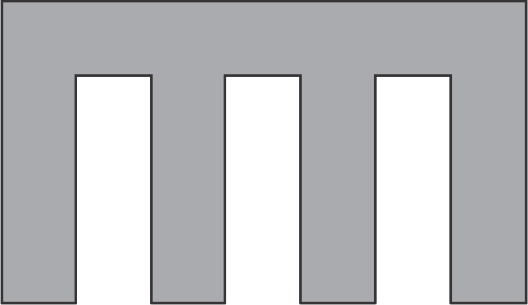
\includegraphics[width=4cm]{imagenes/general2024-I/etapa2/soc/geometria1g24-II.png}
	\end{center}
	
	
	\begin{enumerate}[label=\alph*)]
		\item $2520^\circ$
		\item $1440^\circ$
		\item $2880^\circ$
		\item $2440^\circ$
		\item $1250^\circ$
	\end{enumerate}
	
	\textbf{Respuesta correcta:} a)
	
	\vspace{2mm}
	\textbf{Solucionario:}
	
	Sabemos que: la suma de las medidas de los ángulos interiores es:
	
	$S_i = 180(n-2)$
	
	$S_i = 180(16-2)$
	
	$= 180(14)$
	
	\fbox{$= 2520^\circ$}
	
	
	%========================
	% PREGUNTA 2 (NUEVA)
	%========================
	\item En la figura, las rectas $L_1$ y $L_2$ son paralelas, calcule $a^\circ+b^\circ+c^\circ+d^\circ+e^\circ$.
	
	\begin{center}
		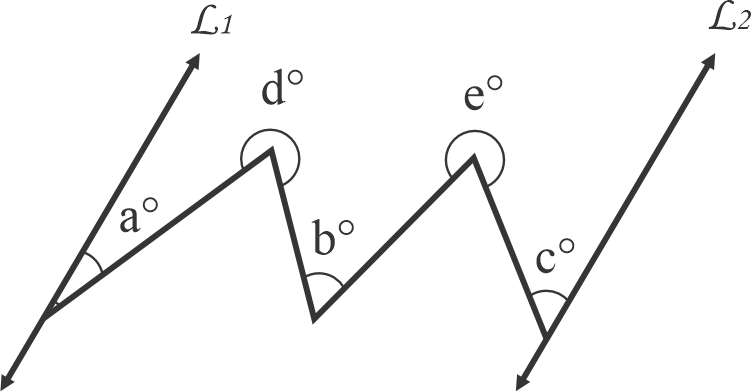
\includegraphics[width=4.5cm]{imagenes/general2024-I/etapa2/soc/geometria2g24-II.png}
	\end{center}
	
	
	\begin{enumerate}[label=\alph*)]
		\item $360^\circ$
		\item $450^\circ$
		\item $540^\circ$
		\item $600^\circ$
		\item $720^\circ$
	\end{enumerate}
	
	\textbf{Respuesta correcta:} e)
	
	\vspace{2mm}
	\textbf{Solucionario:}
	
	\begin{center}
		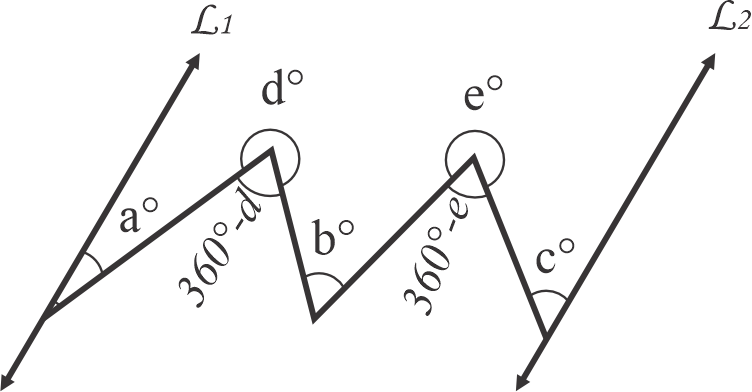
\includegraphics[width=4.5cm]{imagenes/general2024-I/etapa2/soc/geometria2g24-IIr.png}
	\end{center}
	
	De la figura se tiene:
	
	$a^\circ+b^\circ+c^\circ = 360^\circ-d^\circ+360^\circ-e^\circ$
	
	$a^\circ+b^\circ+c^\circ+d^\circ+e^\circ = $\fbox{$720^\circ$}
	
	
\end{enumerate}















\subsection*{Trigonometría}

\begin{enumerate}[resume]
	
	\item En el gráfico, halle $\tan \alpha$.
	
	\begin{center}
		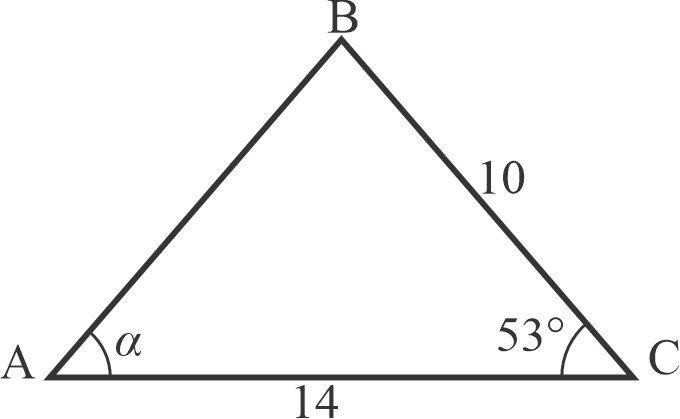
\includegraphics[width=4.5cm]{imagenes/general2024-I/etapa2/soc/trigo1g24-II.png}
	\end{center}
	\begin{enumerate}[label=\alph*)]
		\item 1
		\item $\dfrac{3}{2}$
		\item 2
		\item $\dfrac{3}{4}$
		\item $\dfrac{5}{4}$
	\end{enumerate}
	
	\textbf{Respuesta correcta:} a)
	
	\vspace{2mm}
	\textbf{Solucionario:}\\[1mm]
	\begin{center}
		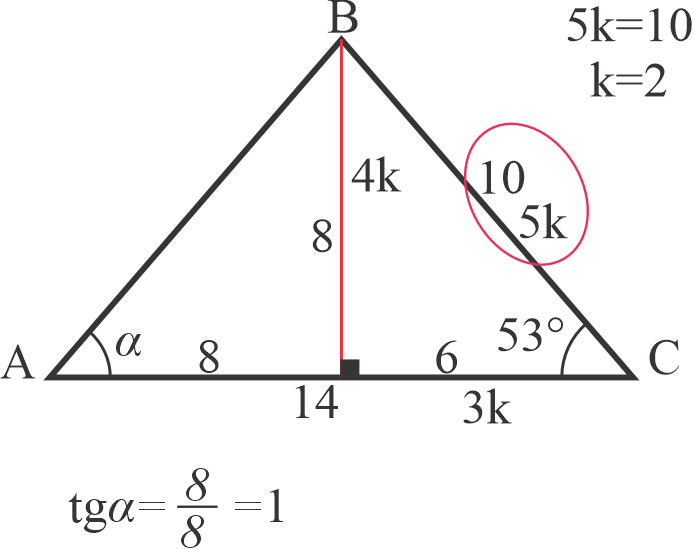
\includegraphics[width=0.4\textwidth]{imagenes/general2024-I/etapa2/soc/trigo1g24-IIr.png}
	\end{center}
	
	\vspace{6mm}
	
	
	
	
	
	\item Calcule el valor de:
	
	\[
	M=\dfrac{4\cos120^\circ-\tg135^\circ}{\sen330^\circ}
	\]
	
	\begin{enumerate}[label=\alph*)]
		\item 6
		\item 2
		\item -3
		\item 3
		\item -2
	\end{enumerate}
	
	\textbf{Respuesta correcta:} b)
	
	\vspace{2mm}
	\textbf{Solucionario:}\\[1mm]
	
	$
	M=\dfrac{4\cos120^\circ-\tg135^\circ}{\sen330^\circ}
	$
	
	$
	M=\dfrac{4\left(-\cos60^\circ\right)-\left(-\tg45^\circ\right)}{-\sen30^\circ}
	$
	
	$
	M=\dfrac{4\left(-\dfrac{1}{2}\right)+1}{-\dfrac{1}{2}}
	$
	
	$
	M=\dfrac{-2+1}{-\dfrac{1}{2}}=$\fbox{$2$}
	
	\vspace{6mm}
	
\end{enumerate}




\subsection*{Física}

\begin{enumerate}[resume]
	
	\item Una esfera de 50 kg se encuentra en equilibrio, tal como se muestra en la figura. Determine la fuerza de reacción en el punto B. Considere superficies lisas.  
	(g = 10 m/s²)
	
	\begin{center}
		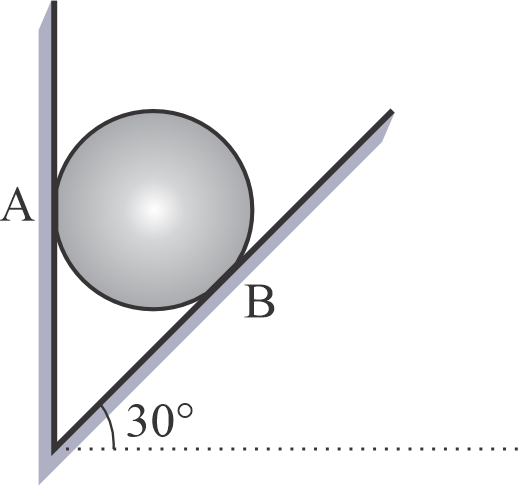
\includegraphics[width=0.3\textwidth]{imagenes/general2024-I/etapa2/soc/fisica1g24-II.png}
	\end{center}
	
	\begin{enumerate}[label=\alph*)]
		\item $\dfrac{3}{\sqrt{3}}$ kN
		\item $\dfrac{2}{\sqrt{3}}$ kN
		\item $\dfrac{\sqrt{3}}{2}$ kN
		\item $\dfrac{\sqrt{3}}{3}$ kN
		\item $\dfrac{\sqrt{2}}{3}$ kN
	\end{enumerate}
	
	\textbf{Respuesta correcta:} d)
	
	\textbf{Solucionario:}
	
	
	Del DCL  
	
	$W = 500\,N$
	
	comparando con  
	
	$K\sqrt{3} = 500\,N$
	
	$K = \dfrac{500}{\sqrt{3}}\,N$
	
	luego:
	
	$R_B = 2K = \dfrac{1000}{\sqrt{3}}\,N$
	
	$R_B = \dfrac{1000\sqrt{3}}{3}\,N =$ \fbox{$ \dfrac{\sqrt{3}}{3}\,kN$}
	
	
	
	
	
	
	
	
	\item José carga una mochila de 400 N de peso sobre su espalda al subir una colina de 30° de inclinación y recorre 40 m en un tiempo de 40 segundos a velocidad constante. Calcule la potencia desarrollada por José para llevar la mochila.
	
	\begin{enumerate}[label=\alph*)]
		\item 300 W
		\item 250 W
		\item 200 W
		\item 100 W
		\item 150 W
	\end{enumerate}
	
	\textbf{Respuesta correcta:} c)
	
	\textbf{Solucionario:}\\[1mm]
	
	
	\begin{center}
		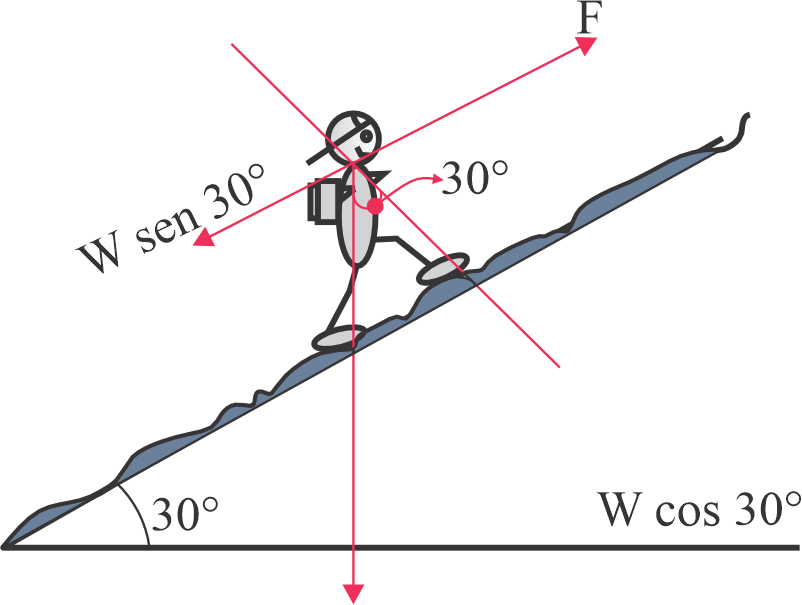
\includegraphics[width=4.5cm]{imagenes/general2024-I/etapa2/soc/fisica2g24-IIr.png}
	\end{center}
	
	\textbf{Solucionario:}
	
	$
	\begin{aligned}
		P &= \dfrac{W}{t} \\
		&= \dfrac{F\cdot d}{t} \\
		&= \dfrac{W\sen 30^\circ \cdot d}{t} \\
		&= \dfrac{400\left(\dfrac{1}{2}\right)(40)}{40} \\
		&=\fbox{ 200\,W}
	\end{aligned}
	$
	
\end{enumerate}







\subsection*{Química}

\begin{enumerate}[resume]
	\item Señale la alternativa que contiene una mezcla, una sustancia compuesta y un elemento, en ese orden.
	
	\begin{enumerate}[label=\Roman*.]
		\item Aire, ácido sulfúrico, agua destilada
		\item Oro de 18 kilates, cloruro de sodio, cobre
		\item Agua destilada, dióxido de carbono, cloro
		\item Agua potable, grafito, ozono
		\item Diamante, glucosa, aluminio.
	\end{enumerate}
	
	\begin{enumerate}[label=\alph*)]
		\item Solo IV
		\item III y IV
		\item Solo II
		\item Solo I
		\item II y IV
	\end{enumerate}
	
	\textbf{Respuesta correcta:} c)
	
	\vspace{2mm}
	\textbf{Solucionario:}\\[1mm]
	
	\begin{itemize}
		\item La mezcla es una reunión de 2 o más componentes, no se puede diferenciar sus componentes a simple vista. El oro de 18 kilates es una mezcla de oro y plata.
		\item Una sustancia compuesta es aquella sustancia formada por una sola clase de moléculas, siendo la molécula formada por átomos diferentes. El cloruro de sodio (NaCl) tiene 2 moléculas diferentes.
		\item Es un elemento químico que se encuentra en la naturaleza, como los metales nativos, ejemplo Cobre, Fierro, etc.)
	\end{itemize}
	
	\vspace{6mm}
	
	\item Señale las proposiciones verdaderas (V) o falsas (F) según corresponda sobre el efecto invernadero.
	
	\begin{enumerate}[label=\Roman*.]
		\item Es el fenómeno mediante el cual se evita que la totalidad de la energía emitida por la superficie terrestre, escape al espacio.
		\item Los gases de efecto invernadero son CO$_2$, CH$_4$, CCl$_2$F$_2$ entre los principales
		\item El gas que contribuye principalmente al efecto invernadero es el CO$_2$.
	\end{enumerate}
	
	\begin{enumerate}[label=\alph*)]
		\item VFV
		\item VVF
		\item VVV
		\item FVV
		\item FVF
	\end{enumerate}
	
	\textbf{Respuesta correcta:} c)
	
	\vspace{2mm}
	\textbf{Solucionario:}
	
	
	Los gases de efecto invernadero son CO$_2$, CH$_4$, CCl$_2$F$_2$ el principal es CO$_2$.
	
	\vspace{6mm}
	
	
\end{enumerate}



\subsection*{Biología y Anatomía}

\begin{enumerate}[resume]
	\item El epitelio simple cilíndrico ciliado se localiza en:
	\begin{enumerate}[label=\alph*)]
		\item Alveolos pulmonares
		\item Pelvis renal
		\item Conjuntiva ocular
		\item Trompas de falopio
		\item Vesícula seminal
	\end{enumerate}
	\textbf{Respuesta correcta:} d)
	
	\vspace{2mm}
	\textbf{Solucionario:}\\[1mm]
	El epitelio de las trompas de Falopio (u oviductos) presenta cilios en su superficie apical que facilitan el transporte del ovocito hacia el útero.
	
	
	\vspace{6mm}
	
	\item ¿Cuál es el polisacárido de reserva en algunos vegetales como el yacón y la alcachofa que está constituido por residuos de fructosa?
	\begin{enumerate}[label=\alph*)]
		\item Pectina
		\item Inulina
		\item Celulosa
		\item Almidón
		\item Ciclodextrina
	\end{enumerate}
	\textbf{Respuesta correcta:} b)
	
	\vspace{2mm}
	\textbf{Solucionario:}\\[1mm]
	La inulina es un fructosano (polímero de fructosa) que sirve como reserva energética en plantas de la familia Asteraceae, a diferencia del almidón que es polímero de glucosa.
	
	
	\vspace{6mm}
\end{enumerate}

\subsection*{Psicología y Filosofía}

\begin{enumerate}[resume]
	\item Si decimos que la mortalidad es algo común en todos los seres vivos, ¿qué operación del pensamiento estamos utilizando?
	\begin{enumerate}[label=\alph*)]
		\item Abstracción
		\item Síntesis
		\item Análisis
		\item Comparación
		\item Generalización
	\end{enumerate}
	\textbf{Respuesta correcta:} e)
	
	\vspace{2mm}
	\textbf{Solucionario:}\\[1mm]
	La generalización es la operación mental que consiste en atribuir una característica observada en elementos particulares a todo un grupo, clase o especie.
	
	\vspace{6mm}
	
	\item Existen pacientes que sufren de amnesia, los cuales a veces son incapaces de recordar un número telefónico, una dirección o el nombre de una persona, pero sí pueden recordar cómo resolver rompecabezas complejos en un tiempo normal, lo cual sería un indicador de que no se encuentra dañada la memoria:
	\begin{enumerate}[label=\alph*)]
		\item semántica.
		\item procedimental.
		\item episódica.
		\item declarativa.
		\item transitoria.
	\end{enumerate}
	\textbf{Respuesta correcta:} b)
	
	\vspace{2mm}
	\textbf{Solucionario:}\\[1mm]
	La memoria procedimental es la encargada de almacenar información sobre procedimientos y habilidades motoras (el "saber cómo"). Esta memoria suele ser más resistente al daño que la declarativa.
	
	\vspace{6mm}
	
	\item En relación con la esencia humana, señale verdad (V) o falsedad (F) de los enunciados.\\
	I. Según Aristóteles, el hombre fuera de la sociedad no podría vivir.\\
	II. Para el maestro de Aristóteles, el hombre nunca muere.\\
	III. Cassire manifiesta que el hombre, antes que se guíe por su razón, se guiaría por su cultura.\\
	IV. Según Nietzsche, el hombre ha roto con su estado natural.\\
	V. Según Cassire, el hombre por naturaleza es un animal simbólico.
	\begin{enumerate}[label=\alph*)]
		\item V V V F V
		\item F F F F V
		\item F V V F V
		\item V V V V F
		\item F F V V V
	\end{enumerate}
	\textbf{Respuesta correcta:} d)
	
	\vspace{2mm}
	\textbf{Solucionario:}\\[1mm]
	I(V): El hombre es un \textit{zoon politikon}. \\
	II(V): Platón postula la inmortalidad del alma. \\
	III(V): La cultura media la relación del hombre con el mundo. \\
	IV(V): Nietzsche afirma que la civilización ha "enfermado" al hombre al separarlo de sus instintos naturales.\\ 
	V(F): Para Cassirer, el simbolismo es una función funcional de la cultura, no un rasgo de la "naturaleza" biológica previa.\\
	
	\vspace{6mm}
	
	\item Determine aquella disciplina en donde nos preguntamos si lo primero es la materia o la idea.
	\begin{enumerate}[label=\alph*)]
		\item Ontología
		\item Epistemología
		\item Axiología
		\item Ética
		\item Gnoseología
	\end{enumerate}
	\textbf{Respuesta correcta:} a)
	
	\vspace{2mm}
	\textbf{Solucionario:}\\[1mm]
	La Ontología (estudio del ser) aborda el problema fundamental de la filosofía: la primacía entre el ser (materia) y el pensar (idea/conciencia).
	
	\vspace{6mm}
\end{enumerate}




\subsection*{Geografía}

\begin{enumerate}[resume]
	\item La capa de la atmósfera del planeta Tierra donde se producen la mayor parte de los fenómenos (vientos, lluvias, nubes, etc.), se denomina:
	\begin{enumerate}[label=\alph*)]
		\item Tropósfera
		\item Termósfera
		\item Estratósfera
		\item Mesósfera
		\item Exósfera
	\end{enumerate}
	\textbf{Respuesta correcta:} a)
	
	\vspace{2mm}
	\textbf{Solucionario:}\\[1mm]
	La tropósfera es la capa en contacto con la superficie terrestre; en ella ocurre la dinámica meteorológica debido a la mayor densidad de gases y vapor de agua.
	
	\vspace{6mm}
	
	\item En los problemas ambientales del Perú, una de las consecuencias directas de la mala disposición de los residuos sólidos es:
	\begin{enumerate}[label=\alph*)]
		\item el gasto económico para solucionar los daños
		\item el conflicto de las autoridades con la población
		\item la corrupción vinculada al manejo de residuos sólidos
		\item la legislación inapropiada
		\item el daño a la salud y al ambiente
	\end{enumerate}
	\textbf{Respuesta correcta:} e)
	
	\vspace{2mm}
	\textbf{Solucionario:}\\[1mm]
	La acumulación de basura a cielo abierto genera focos infecciosos, proliferación de vectores y contaminación de suelos y fuentes de agua, impactando directamente en el ecosistema y la salud pública.
	
	\vspace{6mm}
	
	\item El crecimiento demográfico en los países en que los recursos no han crecido en la misma proporción, es uno de los factores que explica la situación de:
	\begin{enumerate}[label=\alph*)]
		\item la política.
		\item la comunidad nativa.
		\item la pobreza.
		\item los recursos naturales.
		\item los patrones de consumo.
	\end{enumerate}
	\textbf{Respuesta correcta:} c)
	
	\vspace{2mm}
	\textbf{Solucionario:}\\[1mm]
	Según la teoría malthusiana y visiones socioeconómicas modernas, cuando la población crece a un ritmo mayor que la capacidad de producción de recursos y servicios, se agudizan las condiciones de pobreza.
	
	\vspace{6mm}
	
	\item Uno de los efectos del cambio climático en la Tierra es:
	\begin{enumerate}[label=\alph*)]
		\item la disminución del nivel del mar
		\item el incremento de las enfermedades tropicales
		\item la disminución de los fenómenos naturales
		\item el aumento de los recursos naturales
		\item la disminución de la contaminación
	\end{enumerate}
	\textbf{Respuesta correcta:} b)
	
	\vspace{2mm}
	\textbf{Solucionario:}\\[1mm]
	El aumento de la temperatura global permite que vectores (como mosquitos) expandan su hábitat hacia zonas antes frías, incrementando la incidencia de enfermedades como el dengue o la malaria.
	
	\vspace{6mm}
\end{enumerate}

\subsection*{Historia}

\begin{enumerate}[resume]
	\item A partir del periodo de la posguerra con Chile y hasta las primeras décadas del siglo XX, el sector ganadero alcanzó un gran auge incorporándose al ciclo económico de exportación. En el sur peruano, las ciudades de Arequipa, Puno y Cusco experimentaron una creciente prosperidad gracias al:
	\begin{enumerate}[label=\alph*)]
		\item apoyo gubernamental.
		\item sistema de gamonales.
		\item desarrollo de carreteras.
		\item control tributario.
		\item sistema de ferrocarriles.
	\end{enumerate}
	\textbf{Respuesta correcta:} e)
	
	\vspace{2mm}
	\textbf{Solucionario:}\\[1mm]
	La construcción del Ferrocarril del Sur facilitó el transporte de lana (alpaca y oveja) desde el altiplano hacia el puerto de Mollendo para su exportación a Inglaterra, dinamizando la economía regional.
	
	\vspace{6mm}
	
	\item El gran éxito económico de la era del guano en el Perú tuvo como base científica las investigaciones sobre las propiedades fertilizantes del guano de islas que realizaron diversos estudiosos, entre ellos destaca el naturalista peruano:
	\begin{enumerate}[label=\alph*)]
		\item Mariano de Rivero y Ustariz.
		\item Manuel Ascencio Segura.
		\item Mariano Paz Soldan.
		\item Juan Bautista Dueñas.
		\item Pedro Paulet.
	\end{enumerate}
	\textbf{Respuesta correcta:} a)
	
	\vspace{2mm}
	\textbf{Solucionario:}\\[1mm]
	Mariano Eduardo de Rivero y Ustariz fue un prominente científico peruano que realizó los primeros análisis químicos del guano, demostrando su alto valor como abono orgánico en el mercado europeo.
	
	\vspace{6mm}
	
	\item A partir de 1955, la OTAN tuvo como contraparte militar al:
	\begin{enumerate}[label=\alph*)]
		\item gobierno soviético.
		\item Plan Molotov.
		\item COMECON.
		\item Plan Marshall.
		\item Pacto de Varsovia.
	\end{enumerate}
	\textbf{Respuesta correcta:} e)
	
	\vspace{2mm}
	\textbf{Solucionario:}\\[1mm]
	El Pacto de Varsovia fue una alianza de defensa mutua firmada en 1955 por los países del bloque socialista (liderados por la URSS) en respuesta al ingreso de Alemania Occidental a la OTAN.
	
	\vspace{6mm}
	
	\item El alto órgano administrativo para el gobierno de América que nombraba al Virrey y al final de su mandato lo sometía a un juicio de residencia y que además señalaba los lineamientos de la política virreinal fue:
	\begin{enumerate}[label=\alph*)]
		\item la Casa de Contratación de Sevilla
		\item la Intendencia
		\item la Real Audiencia
		\item la Corona Española
		\item el Consejo de Indias
	\end{enumerate}
	\textbf{Respuesta correcta:} e)
	
	\vspace{2mm}
	\textbf{Solucionario:}\\[1mm]
	El Real y Supremo Consejo de Indias tenía funciones legislativas, ejecutivas y judiciales; entre ellas, la selección de altos funcionarios y la fiscalización mediante el juicio de residencia.
	
	\vspace{6mm}
\end{enumerate}


\subsection*{Educación Cívica}

\begin{enumerate}[resume]
	\item Según la Constitución Política de la República del Perú, se suspende el ejercicio de la Presidencia de la República:
	\begin{enumerate}[label=\alph*)]
		\item cuando sale del territorio nacional sin permiso del Congreso.
		\item por su permanente incapacidad moral y física.
		\item cuando ha sido destituido por infracciones contra la Constitución.
		\item por incapacidad temporal del Presidente, declarado por el Congreso.
		\item cuando se acepta su renuncia por el congreso.
	\end{enumerate}
	\textbf{Respuesta correcta:} d)
	
	\vspace{2mm}
	\textbf{Solucionario:}\\[1mm]
	El artículo 114 de la Constitución establece las causales de suspensión, diferenciándolas de la vacancia (incapacidad permanente). La suspensión es temporal y debe ser declarada por el Legislativo.
	
	\vspace{6mm}
	
	\item Puede presentar la acción de inconstitucionalidad:
	\begin{enumerate}[label=\alph*)]
		\item el Consejo de Ministros.
		\item el 15 \% del número legal de Congresistas.
		\item el Defensor del Pueblo.
		\item la Junta de Fiscales.
		\item 2000 ciudadanos con firmas comprobadas por el JNE.
	\end{enumerate}
	\textbf{Respuesta correcta:} c)
	
	\vspace{2mm}
	\textbf{Solucionario:}\\[1mm]
	Según el artículo 203 de la Constitución, el Defensor del Pueblo tiene legitimidad para interponer esta acción ante el Tribunal Constitucional para garantizar que las leyes no vulneren la Carta Magna.
	
	\vspace{6mm}
	
	\item Una de las atribuciones del Presidente de la República según la Constitución es:
	\begin{enumerate}[label=\alph*)]
		\item velar por el respeto de la Constitución y de las leyes.
		\item ejercer el derecho de amnistía.
		\item aprobar tratados de conformidad con la Constitución.
		\item convocar a elecciones generales, parlamentarias, regionales y locales.
		\item aprobar la demarcación territorial que proponga el Poder Ejecutivo.
	\end{enumerate}
	\textbf{Respuesta correcta:} d)
	
	\vspace{2mm}
	\textbf{Solucionario:}\\[1mm]
	De acuerdo al Artículo 118 de la Constitución Política del Perú (inciso 5), el Presidente tiene la facultad de convocar a los procesos electorales en todos los niveles de gobierno. La amnistía es facultad del Congreso, y la opción "a" es un deber general pero la "d" es la atribución técnica específica.
	
	\vspace{6mm}
	
	\item La legislación peruana, señala que la emisión de monedas y billetes es una facultad exclusiva del \rule{1.5cm}{0.4pt} y se realiza a través \rule{1.5cm}{0.4pt}
	\begin{enumerate}[label=\alph*)]
		\item Estado - de la SBS.
		\item BCR - del Estado.
		\item Estado - del BCR.
		\item MEF - del BCR.
		\item Estado - del MEF.
	\end{enumerate}
	\textbf{Respuesta correcta:} c)
	
	\vspace{2mm}
	\textbf{Solucionario:}\\[1mm]
	El Estado peruano ejerce el monopolio de la emisión de dinero a través de su organismo autónomo, el Banco Central de Reserva (BCR), encargado de preservar la estabilidad monetaria.
	
	\vspace{6mm}
\end{enumerate}

\subsection*{Economía}

\begin{enumerate}[resume]
	\item En el Perú, existe un grupo de bancos como el Banco de Crédito del Perú, el Banco Continental, Interbank, etc.; estos bancos son supervisados por la superintendencia de Banca, Seguros y AFP. Según clasificación de la empresa de acuerdo a la propiedad, estos bancos se clasifican como empresas:
	\begin{enumerate}[label=\alph*)]
		\item sociedades anónimas cerradas.
		\item públicas.
		\item sociedades en comandita.
		\item privadas.
		\item mixtas.
	\end{enumerate}
	\textbf{Respuesta correcta:} d)
	
	\vspace{2mm}
	\textbf{Solucionario:}\\[1mm]
	Son empresas privadas porque sus activos y capital pertenecen a inversionistas particulares (personas naturales o jurídicas), con el objetivo de generar rentabilidad para sus dueños.
	
	\vspace{6mm}
	
	\item Ana, para obtener el título de economista, está realizando una tesis acerca del mercado de valores peruanos y observa que en este mercado se vende y compra principalmente:
	\begin{enumerate}[label=\alph*)]
		\item cheques.
		\item depósitos de ahorro.
		\item acciones y bonos.
		\item letras de cambio.
		\item bonos soberanos.
	\end{enumerate}
	\textbf{Respuesta correcta:} c)
	
	\vspace{2mm}
	\textbf{Solucionario:}\\[1mm]
	El mercado de valores (como la Bolsa de Valores de Lima) se especializa en la intermediación directa a través de títulos de participación (acciones) y títulos de deuda (bonos).
	
	\vspace{6mm}
	
	\item Tener una baja tasa de inflación, además de un tipo de cambio estable, está directamente relacionado con un objetivo de la política económica denominado:
	\begin{enumerate}[label=\alph*)]
		\item desarrollo económico.
		\item estabilidad económica.
		\item pleno empleo.
		\item eficiencia distributiva.
		\item equilibrio externo.
	\end{enumerate}
	\textbf{Respuesta correcta:} b)
	
	\vspace{2mm}
	\textbf{Solucionario:}\\[1mm]
	La estabilidad económica se refiere al mantenimiento del equilibrio macroeconómico, evitando crisis inflacionarias o devaluaciones bruscas que afecten la inversión y el consumo.
	
	\vspace{6mm}
	
	\item Una reducción de la demanda de carne de pollo puede deberse a:
	\begin{enumerate}[label=\alph*)]
		\item un incremento del precio de la carne de res.
		\item una variación de los impuestos.
		\item la disminución de su precio.
		\item una mejora de los ingresos del consumidor.
		\item una disminución del precio de la carne de pescado.
	\end{enumerate}
	\textbf{Respuesta correcta:} e)
	
	\vspace{2mm}
	\textbf{Solucionario:}\\[1mm]
	El pescado es un bien sustituto del pollo. Si el precio del sustituto baja, los consumidores dejarán de comprar pollo para adquirir pescado, reduciendo así la demanda del primero.
	
	\vspace{6mm}
\end{enumerate}


\subsection*{Comunicación}

\begin{enumerate}[resume]
	\item Era de postura mediana, de anchas espaldas, fuertemente labrado y músculos. El cuerpo estaba deformado por el trabajo, caminaba con la cabeza erguida, la espalda combada y el vientre hacia adelante.\\
	\\
	¿A qué tipo de texto corresponde el fragmento?
	\begin{enumerate}[label=\alph*)]
		\item Narrativo
		\item Expositivo
		\item Descriptivo
		\item Argumentativo
		\item Instructivo
	\end{enumerate}
	\textbf{Respuesta correcta:} c)
	
	\vspace{2mm}
	\textbf{Solucionario:}\\[1mm]
	El fragmento se centra en detallar las características físicas de un sujeto (prosopografía), lo cual es la función principal del texto descriptivo.
	
	\vspace{6mm}
	
	\item El licenciado Jorge, director de su escuela profesional, decide felicitar al coordinador de responsabilidad social por haber participado en la parada universitaria.\\
	\\
	¿Qué tipo de documento redactará?
	\begin{enumerate}[label=\alph*)]
		\item Informe
		\item Solicitud
		\item Acta
		\item Memorando
		\item Oficio
	\end{enumerate}
	\textbf{Respuesta correcta:} e)
	
	\vspace{2mm}
	\textbf{Solucionario:}\\[1mm]
	El oficio es el documento utilizado por autoridades para comunicaciones oficiales (felicitaciones, agradecimientos, gestiones) entre dependencias o hacia el exterior.
	
	\vspace{6mm}
	
	\item La telenovela es un género de la televisión que narra historias ficticias.\\
	\\
	El enunciado:
	\begin{enumerate}[label=\alph*)]
		\item relata un hecho.
		\item defiende una opinión.
		\item explica un fenómeno.
		\item describe un objeto.
		\item reproduce una interacción verbal.
	\end{enumerate}
	\textbf{Respuesta correcta:} c)
	
	\vspace{2mm}
	\textbf{Solucionario:}\\[1mm]
	El enunciado tiene una función informativa o referencial; busca definir o explicar qué es la telenovela dentro del contexto televisivo.
	
	\vspace{6mm}
	
	\item Consiste en organizar información relevante alrededor de una idea principal o postura que aparece en un texto. Permite desarrollar habilidades de manejo de información, análisis de situaciones y pensamiento crítico.
	\begin{enumerate}[label=\alph*)]
		\item Espina de Ishikawa
		\item Mapa semántico
		\item Cruz categorial
		\item Diagrama de flujo
		\item Mapa conceptual
	\end{enumerate}
	\textbf{Respuesta correcta:} c)
	
	\vspace{2mm}
	\textbf{Solucionario:}\\[1mm]
	La cruz categorial es un organizador visual que permite analizar un tema central (ubicado en el centro) relacionándolo con sus causas, consecuencias, argumentos y propósitos.
	
	\vspace{6mm}
\end{enumerate}

\subsection*{Literatura}

\begin{enumerate}[resume]
	\item ¿Cómo termina la novela "El viejo y el mar" de Hemingway?
	\begin{enumerate}[label=\alph*)]
		\item Manolín recibe a Santiago en la playa y admira el espinazo del pez aguja, que es todo lo que quedó.
		\item Santiago despierta en su cabaña, pues todo había sido un sueño.
		\item Santiago y Manolín parten de nuevo para superar la hazaña del viejo.
		\item Santiago muere en los arenales del mar.
		\item Una mujer comenta acerca del espinazo del Pez.
	\end{enumerate}
	\textbf{Respuesta correcta:} a)
	
	\vspace{2mm}
	\textbf{Solucionario:}\\[1mm]
	Tras la lucha contra los tiburones, Santiago llega a la orilla solo con el esqueleto del gran pez. Su leal aprendiz, Manolín, lo recibe y lo cuida, reconociendo su valor.
	
	\vspace{6mm}
	
	\item Se constituye como el movimiento literario más importante de España se caracteriza por su hermetismo, uso recargado de adornos estéticos y complejos en su composición. ejm. El ingenioso don Quijote de la Mancha.
	\begin{enumerate}[label=\alph*)]
		\item Neo clasismo
		\item Realismo
		\item Barroquismo
		\item Costumbrismo
		\item Romanticismo
	\end{enumerate}
	\textbf{Respuesta correcta:} c)
	
	\vspace{2mm}
	\textbf{Solucionario:}\\[1mm]
	El Barroco español destaca por la sofisticación formal (culteranismo y conceptismo), el contraste y la visión pesimista de la realidad, presente en la madurez de Cervantes.
	
	\vspace{6mm}
	
	\item ¿Qué figura literaria se destaca en los versos de "La vida es un sueño"?\\
	\\
	Hace el arroyo, culebra\\
	que entre flores se desata\\
	entre las flores se quiebra
	\begin{enumerate}[label=\alph*)]
		\item símil
		\item metonimia
		\item metáfora
		\item hipérbole
		\item hipérbaton
	\end{enumerate}
	\textbf{Respuesta correcta:} c)
	
	\vspace{2mm}
	\textbf{Solucionario:}\\[1mm]
	Se emplea la metáfora al identificar al arroyo directamente con una "culebra" por su forma serpenteante, sin usar nexos como "parece" o "como".
	
	\vspace{6mm}
	
	\item "Los miserables" y "Nuestra Señora de París" obras de Víctor Hugo, pertenecen al género:
	\begin{enumerate}[label=\alph*)]
		\item épico.
		\item lírico.
		\item narrativo.
		\item expositivo.
		\item dramático.
	\end{enumerate}
	\textbf{Respuesta correcta:} c)
	
	\vspace{2mm}
	\textbf{Solucionario:}\\[1mm]
	Al ser novelas que relatan una secuencia de hechos a través de un narrador en prosa, se ubican dentro del género narrativo moderno.
	
	\vspace{6mm}
\end{enumerate}











\subsection*{Razonamiento Matemático}

\begin{enumerate}[resume]
	
	\item En el gráfico, se muestran dos cuadrados mágicos aditivos de $3 \times 3$. Calcule $A+B+C-(D+E+F)$
	
	\begin{center}
		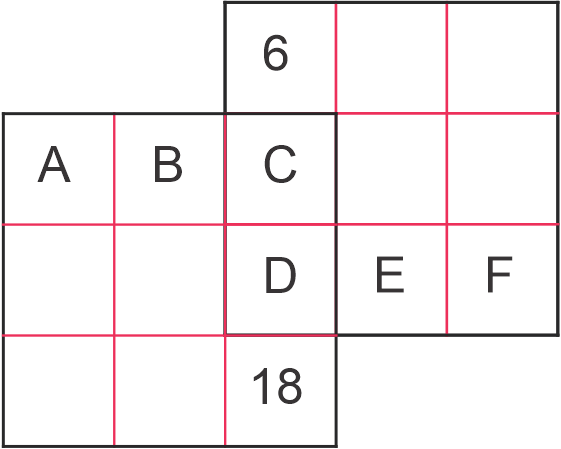
\includegraphics[width=3.5cm]{imagenes/general2024-I/etapa2/soc/rm1g24-II.png}
	\end{center}
	
	\begin{enumerate}[label=\alph*)]
		\item 18
		\item 12
		\item 24
		\item 9
		\item 8
	\end{enumerate}
	\textbf{Respuesta correcta:} b)
	
	\vspace{2mm}
	
	\textbf{Solucionario:}


	De la figura y el cuadrado mágico de la izquierda:
	
	\begin{equation*}
		A + B = D + 18 \quad \Rightarrow \quad A + B - D = 18 \quad \dots (I)
	\end{equation*}
	
	De la figura y el cuadrado mágico de la derecha:
	\begin{equation*}
		G + C = E + F \quad \Rightarrow \quad C - E - F = -G \quad \dots (II)
	\end{equation*}
	Sumando (I) y (II):
	\begin{align*}
		A + B - D + C - E - F &= 18 - 6 \\
		A + B + C - D - E - F &= 12 \\
		A + B + C - (D + E + F) &= 12
	\end{align*}
	
	
	
	
	
	\vspace{6mm}
	
	\item Paula recomendada para el manejo de dinero, recibió 100 billetes de $S/ 20$, $S/ 50$ y $S/ 100$, y el monto recibido es de $S/ 7300$. El número de billetes de $S/ 20$ es la mitad de los de $S/ 50$. ¿Cuál es el número de billetes de $S/ 100$?
	\begin{enumerate}[label=\alph*)]
		\item 53
		\item 55
		\item 50
		\item 57
		\item 65
	\end{enumerate}
	\textbf{Respuesta correcta:} b)
	
	\vspace{2mm}
	
	\textbf{Solucionario:}
	
	El total de billetes es 100
	\begin{center}
		\begin{tabular}{|c|c|c|c|c|}
			\hline
			& $S/. 20$ & $S/. 50$ & $S/. 100$ & TOTAL \\ \hline
			\# de billetes & $x$ & $2x$ & $100 - 3x$ & $100$ \\ \hline
			Monto & $20x$ & $50(2x)$ & $100(100 - 3x)$ & $7300$ \\ \hline
		\end{tabular}
	\end{center}
	
	Planteando:
	\begin{align*}
		2x + 5(2x) + 10(100 - 3x) &= 730 \\
		18x = 270 \quad \Rightarrow \quad &x = 15
	\end{align*}
	
	$\therefore$ \# de billetes de $S/. 100$
	\begin{equation*}
		\text{es } 100 - 3x = 100 - 3(15) = \fbox{55}
	\end{equation*}
	
	
	
	
	\vspace{6mm}
	
	\item Dos relojes se sincronizan a las 12 del mediodía. Si uno de ellos se atrasa 12 minutos cada hora con respecto a otro, ¿cuánto tiempo transcurrirá hasta que ambos relojes marquen la misma hora?
	\begin{enumerate}[label=\alph*)]
		\item 2,0 días
		\item 1,5 días
		\item 2,5 días
		\item 3,5 días
		\item 3,0 días
	\end{enumerate}
	\textbf{Respuesta correcta:} c)
	
	\vspace{2mm}
	
	\textbf{Solucionario:}
	
	Dato: Uno de los relojes se atrasa 12 minutos por cada hora.
	
	\begin{center}
		\begin{tabular}{c|c}
			Se atrasa & $1 \text{ h.}$ \\ \hline
			$12 \text{ min}$ & $60 \text{ h}$ \\
			$720 \text{ min}$ & 
		\end{tabular}
	\end{center}
	
	$\hookrightarrow$ Se debe atrasar $720$ minutos para que marque la misma hora.
	
	\begin{equation*}
		\dfrac{720}{12} = 60
	\end{equation*}
	
	$60 \text{ h.}$ es $2,5$ días.
	
	$\therefore$ Ambos relojes volverán a marcar la misma hora dentro de \fbox{$2,5$} días.
	
	
	\item Calcule el área de la región sombreada, donde los arcos son de circunferencia
	
	
	\begin{center}
		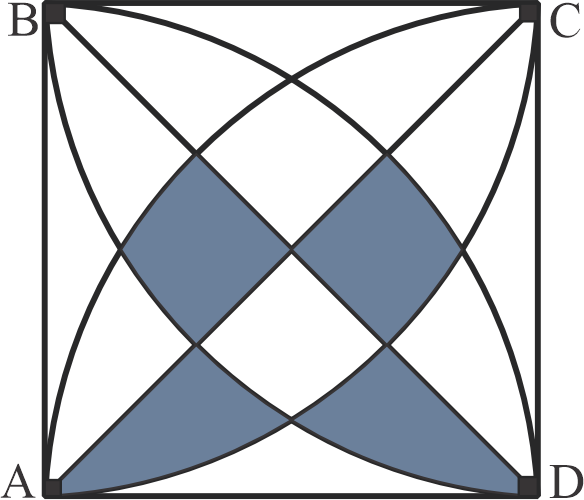
\includegraphics[width=0.3\textwidth]{imagenes/general2024-I/etapa2/soc/rm4g24-II.png}
	\end{center}
	
	\begin{enumerate}[label=\alph*)]
		\item $2(\pi-4)u^2$
		\item $3(2\pi-1)u^2$
		\item $6(\pi-2)u^2$
		\item $4(\pi-2)u^2$
		\item $5(\pi-4)u^2$
	\end{enumerate}	
	\textbf{Respuesta correcta:} d)
	
	\vspace{2mm}
	\textbf{Solucionario:}
	
	\begin{center}
		\begin{minipage}{0.45\textwidth}
			\begin{minipage}{0.45\textwidth}
				\centering
				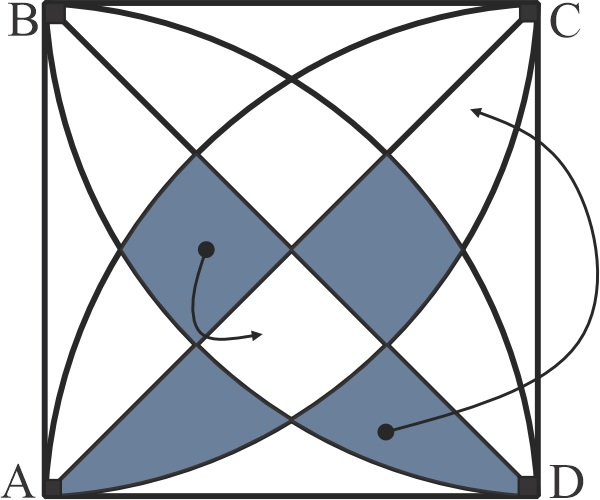
\includegraphics[width=3.5cm]{imagenes/general2024-I/etapa2/soc/rm4g24-IIr.png}
			\end{minipage}
			
			\vspace{6mm}
		\end{minipage}
		\hfill
		\begin{minipage}{0.45\textwidth}
			\centering
			S= Área de la cuarta parte de una circunferencia  menos al área de un triángulo\\
			
			$=\dfrac{\pi 4^2}{4}-\dfrac{4 \text{x} 4}{2}$\\
			
			$= 4 \pi -8$\\
			
			=\fbox{$4(\pi -2)u^2$}

		\end{minipage}
	\end{center}
	
	
	
	
	\item Halle el total de triángulos en la figura mostrada.
	
	\begin{center}
		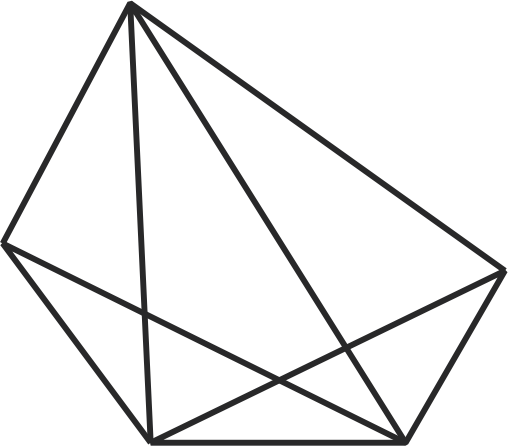
\includegraphics[width=0.3\textwidth]{imagenes/general2024-I/etapa2/soc/rm5g24-II.png}
	\end{center}
	
	
	\begin{enumerate}[label=\alph*)]
		\item 14
		\item 10
		\item 22
		\item 18
		\item 20
	\end{enumerate}
	\textbf{Respuesta correcta:} e)
	
	\vspace{2mm}
	\textbf{Solucionario:}
	
	Contando por regiones: 
	
	De 1 región: 1, 2, 3, 4, 5, 6, 7 $\rightarrow$ 7 
	
	De 2 regiones: 12, 23, 34, 45, 56, 67, 3X, 5X $\rightarrow$ 8 
	
	De 3 regiones: 234, 456, 1X5, 3X7 $\rightarrow$ 4 
	
	De 4 regiones: 345X $\rightarrow$ 1 
	
	Total = $7 + 8 + 4 + 1 = $\fbox{$20$}
	
	
	
	\vspace{6mm}
	
	\item Un estudiante tiene que resolver solamente 8 preguntas de 10 en un examen. ¿Cuántas maneras de escoger las preguntas tiene el estudiante?
	\begin{enumerate}[label=\alph*)]
		\item 10
		\item 35
		\item 45
		\item 25
		\item 20
	\end{enumerate}
	\textbf{Respuesta correcta:} c)
	
	\vspace{2mm}
	\textbf{Solucionario:}
	
	Es una combinatoria ya que no importa el orden de selección: 
	
	$C_{8}^{10} = \dfrac{10!}{(10-8)! \cdot 8!} = \dfrac{10 \times 9 \times 8!}{2! \cdot 8!} =$\fbox{$ 45$}
	
	\vspace{6mm}
	
	
	
	\vspace{6mm}
	
\end{enumerate} 	












































\subsection*{Razonamiento Verbal}

\begin{enumerate}[resume]
	\item En la palabra taquigrafía, la raíz griega \textit{taqui} significa:
	\begin{enumerate}[label=\alph*)]
		\item veloz.
		\item palabra.
		\item escritura.
		\item digitar.
		\item símbolos.
	\end{enumerate}
	\textbf{Respuesta correcta:} a)
	
	\vspace{2mm}
	\textbf{Solucionario:}\\[1mm]
	La raíz griega \textit{tachys} significa "rápido" o "veloz". Por lo tanto, la taquigrafía es el método de escritura rápida mediante signos y abreviaturas.
	
	\vspace{6mm}
	
	\item Julio Ramón Ribeyro - La tentación del fracaso (Diario): "¡Diablos! Si las últimas treinta o cuarenta novelas que he tratado de leer no las he terminado, es porque deben tener algún defecto, algo que les impiden colmar mis expectativas."\\
	\\
	¿A qué se deben las lecturas inconclusas del autor?
	\begin{enumerate}[label=\alph*)]
		\item A sus limitaciones académicas.
		\item Al estilo particular de la prosa.
		\item A la diversidad de los temas.
		\item A lo defectuoso de las novelas leídas.
		\item Al exagerado gusto Literario del autor.
	\end{enumerate}
	\textbf{Respuesta correcta:} d)
	
	\vspace{2mm}
	\textbf{Solucionario:}\\[1mm]
	El autor indica explícitamente que la razón por la que no termina las novelas es porque estas "deben tener algún defecto" que impide que cumplan sus expectativas.
	
	\vspace{6mm}
	
	\item Complete la oración:\\
	\\
	La vocación es el \rule{2cm}{0.4pt} íntimo que siente una persona hacia un tipo del \rule{2cm}{0.4pt}.
	\begin{enumerate}[label=\alph*)]
		\item dilema - actividad
		\item objetivo - profesión
		\item impulso - quehacer
		\item interés - accionar
		\item acto - labor
	\end{enumerate}
	\textbf{Respuesta correcta:} c)
	
	\vspace{2mm}
	\textbf{Solucionario:}\\[1mm]
	La palabra "impulso" se ajusta a la naturaleza interna de la vocación, mientras que "quehacer" se refiere a la actividad o tarea a la que uno se dedica.
	
	\vspace{6mm}
	
	\item El sinónimo de SINDÉRESIS es:
	\begin{enumerate}[label=\alph*)]
		\item acentuación.
		\item resumen.
		\item omisión.
		\item interés.
		\item juicio.
	\end{enumerate}
	\textbf{Respuesta correcta:} e)
	
	\vspace{2mm}
	\textbf{Solucionario:}\\[1mm]
	La sindéresis es la capacidad de juzgar rectamente o tener buen sentido, por lo que su sinónimo más preciso es "juicio".
	
	\vspace{6mm}
	
	\item Identifique el par analógico:\\
	\\
	DISIPACIÓN : GASTAR ::
	\begin{enumerate}[label=\alph*)]
		\item verborrea : hablar.
		\item tempestad : llover.
		\item carrera : trasladar.
		\item negligencia : actuar.
		\item apetito : comer.
	\end{enumerate}
	\textbf{Respuesta correcta:} a)
	
	\vspace{2mm}
	\textbf{Solucionario:}\\[1mm]
	La relación es de exceso o intensidad. Disipación es el gasto excesivo y desmedido, así como la verborrea es el hablar excesivo y redundante.
	
	\vspace{6mm}
	
	\item \textbf{PLAN DE REDACCIÓN}\\
	\\
	\textbf{Importancia de la sintaxis}
	\begin{itemize}[label={}]
		\item I. Etimológicamente, sintaxis quiere decir con orden.
		\item II. El dominio de la sintaxis influye en el orden del pensamiento.
		\item III. La sintaxis es parte de la gramática que enseña a ordenar las palabras para que el sentido de la oración sea completo.
		\item IV. El maestro hará ver que los pensamientos no funcionan por medio de palabras aisladas, sino palabras relacionadas unas con otras.
	\end{itemize}
	\begin{enumerate}[label=\alph*)]
		\item I - II - IV - III
		\item III - II - I - IV
		\item III - I - II - IV
		\item I - III - II - IV
		\item I - III - IV - II
	\end{enumerate}
	\textbf{Respuesta correcta:} d)
	
	\vspace{2mm}
	\textbf{Solucionario:}\\[1mm]
	El orden lógico comienza con la etimología (I), sigue con la definición gramatical (III), continúa con la importancia intelectual o cognitiva (II) y finaliza con la aplicación práctica en el aula (IV).
	
	\vspace{6mm}
\end{enumerate}


\subsection*{Inglés}

\begin{enumerate}[resume]
	\item Choose one alternative that it has one adverb of possibility.
	\begin{enumerate}[label=\alph*)]
		\item I need to call to my teacher.
		\item In my free time I fix cellphones.
		\item Maybe he is a lawyer.
		\item She has dread to go at the hospital.
		\item He like to stay in home.
	\end{enumerate}
	\textbf{Respuesta correcta:} c)
	
	\vspace{2mm}
	\textbf{Solucionario:}\\[1mm]
	La palabra "Maybe" (tal vez/quizás) es un adverbio de posibilidad que se utiliza para indicar que algo es probable pero no seguro. Las demás alternativas son oraciones enunciativas sin este tipo de adverbios.
	
	\vspace{6mm}
	
	\item What is the antonym of "ugly"?
	\begin{enumerate}[label=\alph*)]
		\item smelly
		\item beautiful
		\item good
		\item bad
		\item white
	\end{enumerate}
	\textbf{Respuesta correcta:} b)
	
	\vspace{2mm}
	\textbf{Solucionario:}\\[1mm]
	"Ugly" significa feo/a. Su antónimo directo es "beautiful", que significa hermoso/a o bello/a.
	
	\vspace{6mm}
\end{enumerate}

\subsection*{Quechua y Aimara}

\begin{enumerate}[resume]
	\item ¿Hayk'a raphrakunayuqtaq wallpakunari kanku? / ¿Wallpaxa qawqha chhiqanisa?
	\begin{enumerate}[label=\alph*)]
		\item Iskay raphrakunayuq / Pä chhiqani.
		\item Kimsa raphrakunayuq / Kimsa chhiqani.
		\item Tawa Raphrakunayuq / Pusi chhiqani.
		\item Pichqa Raphrakunayuq / Phisqa chhiqani.
		\item Suqta Raphrakunayuq / Suxta chhiqani.
	\end{enumerate}
	\textbf{Respuesta correcta:} a)
	
	\vspace{2mm}
	\textbf{Solucionario:}\\[1mm]
	La pregunta inquiere por la cantidad de alas de una gallina. En Quechua, "Iskay" significa dos, y en Aimara, "Pä" también significa dos. Naturalmente, las gallinas tienen dos alas.
	
	\vspace{6mm}
	
	\item ¿Mayqin saphi hunt'achiktaq achkayachiqri? / ¿Kawkiri askichirisa waljaptayi?
	\begin{enumerate}[label=\alph*)]
		\item kuna / naka
		\item wan / mpi
		\item pi / na
		\item paq / taki
		\item man / ru
	\end{enumerate}
	\textbf{Respuesta correcta:} a)
	
	\vspace{2mm}
	\textbf{Solucionario:}\\[1mm]
	Se pregunta por los sufijos pluralizadores. En el Quechua Cusco-Collao, el sufijo pluralizador es "-kuna" (ej. \textit{allqu-kuna}), y en el Aimara es "-naka" (ej. \textit{anu-naka}).
	
	\vspace{6mm}
\end{enumerate}

\newpage


\section*{Ejercicios Propuestos }

\addcontentsline{toc}{subsection}{Ejercicios Propuestos}

\begin{enumerate}
	
	\item Una empresa decide invertir un capital de \$120 000 en dos proyectos: el proyecto A paga una tasa de interés del 5\% anual y el proyecto B, de mayor riesgo, paga una tasa anual del 8\%. Si la empresa desea un ingreso total anual de \$8550, ¿cuánto invirtió en cada proyecto?
	\begin{enumerate}[label=\alph*)]
		\item \$40 000 ; \$80 000
		\item \$80 000 ; \$40 000
		\item \$95 000 ; \$25 000
		\item \$30 000 ; \$90 000
		\item \$35 000 ; \$85 000
	\end{enumerate}
	
	\item Un maestro de obras deberá construir un pequeño jardín interior en cada uno de los 24 pisos de un edificio. Por la dificultad de trasladar los materiales a cada uno de los pisos, llega al siguiente acuerdo con el propietario del edificio: por cada jardín construido, cobrará S/100 más que lo que cobró por el piso anterior. Si por el jardín del quinto piso cobrará S/2400, ¿cuántos soles cobrará por toda la obra concluida?
	\begin{enumerate}[label=\alph*)]
		\item S/ 75 600
		\item S/ 80 000
		\item S/ 71 300
		\item S/ 67 100
		\item S/ 82 500
	\end{enumerate}
	
	\item Halle el valor de $x$ en la ecuación:
	
	$\left(\dfrac{9}{25}\right)^{x+1}\left(\dfrac{125}{27}\right)^{x+2}=\dfrac{5}{3}$
	
	\begin{enumerate}[label=\alph*)]
		\item $-1$
		\item 1
		\item $-2$
		\item 3
		\item $-3$
	\end{enumerate}
	
	\item Un comerciante de bebidas rehidratantes analiza sus registros de ventas y encuentra que si vende $x$ bebidas en un día, su ganancia (en dólares) está dada por:
	
	$P(x)=3x-\dfrac{1}{1000}x^2-1800$
	
	¿Cuál es su ganancia máxima por día y cuántas bebidas debe vender para obtener dicha ganancia?
	
	\begin{enumerate}[label=\alph*)]
		\item \$ 500 ; 1500
		\item \$ 350 ; 1200
		\item \$ 200 ; 1000
		\item \$ 450 ; 1500
		\item \$ 500 ; 1000
	\end{enumerate}
	
	\item De la figura, calcula $AT$.
	
	\begin{center}
		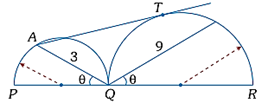
\includegraphics[width=4.5cm]{imagenes/propuestos/geo7.png}
	\end{center}
	
	\begin{enumerate}[label=\alph*)]
		\item $3\sqrt{3}$
		\item 12
		\item 6
		\item 8
		\item 4
	\end{enumerate}
	
	\item En el triángulo mostrado, determina $x$.
	
	\begin{center}
		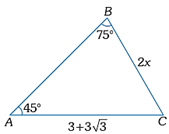
\includegraphics[width=3.5cm]{imagenes/propuestos/geo8.png}
	\end{center}
	
	\begin{enumerate}[label=\alph*)]
		\item $\sqrt{3}$
		\item 3
		\item 2
		\item $\sqrt{3}+1$
		\item $1+\sqrt{6}$
	\end{enumerate}
	
	\item Indicar el valor de verdad de las siguientes proposiciones:
	
	$(\ )$ El seno es creciente en el II C\\
	$(\ )$ El coseno es creciente en el III C\\
	$(\ )$ La tangente es decreciente en el IV C
	
	\begin{enumerate}[label=\alph*)]
		\item V V F
		\item V F V
		\item F F V
		\item F V F
		\item F V V
	\end{enumerate}
	
	\item Si $\tan^2 x+\cot^2 x=2$, donde $x$ pertenece al cuarto cuadrante, halle el valor de:
	
	$U=\dfrac{\cot^{21}x+\tan^{31}x+6}{\tan^{11}x+\cot^{13}x+3}$
	
	\begin{enumerate}[label=\alph*)]
		\item 8
		\item 4
		\item $-4$
		\item 1
		\item 3
	\end{enumerate}
	
	\item La intensidad de corriente que circula por un conductor es de $2\ \mu A$. ¿Qué tiempo demorarán $5\times 10^{13}$ electrones en cruzar una determinada sección transversal del conductor?
	\begin{enumerate}[label=\alph*)]
		\item 1 s
		\item 2 s
		\item 3 s
		\item 4 s
		\item 5 s
	\end{enumerate}
	
	\item El sistema dinámico mostrado en la figura acelera uniformemente tal que el péndulo de masa $m$ se mantiene en equilibrio. Determinar la aceleración de dicho sistema. $(g=10,0\ \text{m/s}^2)$
	
	\begin{center}
		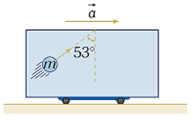
\includegraphics[width=3.5cm]{imagenes/propuestos/fi8.png}
	\end{center}
	
	\begin{enumerate}[label=\alph*)]
		\item 1,0 m/s$^{-2}$
		\item 5,8 m/s$^{-2}$
		\item 9,6 m/s$^{2}$
		\item 10,0 m/s$^{-2}$
		\item 13,3 m/s$^{2}$
	\end{enumerate}
	
	\item En una fábrica se embotella oxígeno gaseoso $(O_2)$ a $27^\circ C$ y 60 atmósferas en cilindros de 0,82 L. Determine la masa del oxígeno que va en los cilindros.
	\begin{enumerate}[label=\alph*)]
		\item 30 g
		\item 520 g
		\item 64 g
		\item 11,2 g
		\item 300 g
	\end{enumerate}
	
	\item Determine la cantidad de calor necesario que se debe suministrar a 500 g de hielo que se encuentra a $0^\circ C$ para convertirlos en agua a $20^\circ C$.
	\begin{enumerate}[label=\alph*)]
		\item 60 kcal
		\item 55 kcal
		\item 50 kcal
		\item 80 kcal
		\item 70 kcal
	\end{enumerate}
	
	\item Una de las alternativas se encuentra entre los oligosacáridos:
	\begin{enumerate}[label=\alph*)]
		\item Quitobiosa
		\item Galactosa
		\item Ribosa
		\item Eritrosa
		\item Xilosa
	\end{enumerate}
	
	\item En la intoxicación por monóxido de carbono, una concentración de carboxihemoglobina de 10 a 20\% produce:
	\begin{enumerate}[label=\alph*)]
		\item dolor de cabeza.
		\item irritabilidad.
		\item desmayo.
		\item confusión.
		\item Muerte
	\end{enumerate}
	
	\item ¿Qué nombre se les ha dado a las democracias que hacen uso de la tecnología, como el voto electrónico, para consolidarse como tales?
	\begin{enumerate}[label=\alph*)]
		\item Puras
		\item Participativas
		\item Digitales
		\item Representativas
		\item Directas
	\end{enumerate}
	
	\item Identifica las emociones en la siguiente relación:
	
	I. alegría\\
	II. odio\\
	III. miedo\\
	IV. amor
	
	\begin{enumerate}[label=\alph*)]
		\item III - IV
		\item I - II
		\item I - IV
		\item II - III
		\item I - III
	\end{enumerate}
	
	\item Son ríos de Europa que vierten sus aguas al Mar Caspio:
	
	1. Don\\
	2. Volga\\
	3. Onega\\
	4. Ural\\
	5. Loira
	
	Son ciertas:
	\begin{enumerate}[label=\alph*)]
		\item 1, 5 y 4
		\item 1, 3 y 5
		\item 2, 1 y 3
		\item 1 y 3
		\item 2 y 4
	\end{enumerate}
	
	\item Con respecto a la Selva Baja, indique lo correcto.
	\begin{enumerate}[label=\alph*)]
		\item Es el sector más poblado de la Amazonía.
		\item Posee la mayor biodiversidad.
		\item Su clima es templado cálido y húmedo.
		\item Se le conoce como la región de los pongos.
		\item Los ríos la recorren de manera torrentosa.
	\end{enumerate}
	
	\item Un ciudadano venezolano, con residencia prolongada y formal en el Perú, siente que el Estado vulnera sus derechos al impedirle acceder a un cargo en el aparato estatal para el cual se sabe calificado. Habiendo agotado las instancias nacionales de justicia, según la Convención Americana sobre Derechos Humanos, dicho ciudadano, ¿está habilitado para que su caso lo vea la Corte Interamericana de Derechos Humanos?
	\begin{enumerate}[label=\alph*)]
		\item No, debido a que Venezuela se apartó de la Convención Americana sobre Derechos Humanos en 2012.
		\item Sí, debido a que el Perú está adscrito a la Convención Americana sobre Derechos Humanos.
		\item Sí, siempre que la Comisión Interamericana de Derechos Humanos asuma su caso como propio.
		\item No, porque dicho ciudadano no ha acatado lo dispuesto por las instancias internas de justicia.
		\item Sí, en la medida que dicho ciudadano haya tramitado oportunamente su nacionalidad peruana.
	\end{enumerate}
	
	
		\item Son tributos administrados por los gobiernos locales.
	
	1. alcabala\\
	2. impuesto general a las ventas\\
	3. impuesto selectivo al consumo\\
	4. predial\\
	5. arbitrios
	
	Son ciertas:
	\begin{enumerate}[label=\alph*)]
		\item 1, 2 y 3.
		\item 1, 3 y 4.
		\item 1, 4 y 5.
		\item 2, 3 y 5.
		\item 3, 4 y 5.
	\end{enumerate}
	
	\item Las funciones que debe cumplir el dinero son:
	
	1. unidad de cuenta\\
	2. medio de pago\\
	3. durabilidad\\
	4. depósito de valor\\
	5. manuabilidad
	
	Son ciertas:
	\begin{enumerate}[label=\alph*)]
		\item 1, 2 y 3
		\item 1, 2 y 4
		\item 1, 2 y 5
		\item 2, 3 y 4
		\item 3 y 5
	\end{enumerate}
	
	\item Durante la época inca, las mujeres escogidas por su belleza física y sus habilidades para el tejido eran conocidas como:
	\begin{enumerate}[label=\alph*)]
		\item illapas
		\item tumipancas
		\item quillas
		\item acllas
		\item pariacacas
	\end{enumerate}
	
	\item La estrategia económica de Estados Unidos para promover el financiamiento, la reconstrucción y reactivación económica de los países de Europa occidental después de la II guerra mundial se denominó:
	\begin{enumerate}[label=\alph*)]
		\item Plan Dodge
		\item Plan Marshall
		\item Alianza para el Progreso
		\item OTAN
		\item Plan Roosevelt
	\end{enumerate}
	
	
	
	
	\item Identifica al filósofo italiano que creó el concepto de “hegemonía cultural”, concepto muy usado actualmente.
	\begin{enumerate}[label=\alph*)]
		\item Antonio Gramsci
		\item Marsilio Ficino
		\item Giambattista Vico
		\item René Descartes
		\item Nicolás de Cusa
	\end{enumerate}
	
	\item En “El banquete”, luego de la conversación con el presidente, a Don Fernando se le prometen dos cosas:
	
	1. una embajada en París\\
	2. asistir, citado él también, al día siguiente a la reunión de diputados\\
	3. una embajada en Roma\\
	4. Don Fernando citará a todos sus ministros para el tema acordado\\
	5. la embajada de Italia y arreglar los caminos a su tierra
	
	Son ciertas:
	\begin{enumerate}[label=\alph*)]
		\item 1 y 2
		\item 1 y 3
		\item 2 y 3
		\item 3 y 4
		\item 4 y 5
	\end{enumerate}
	
	\item En \textit{Cien años de soledad}, y casi al final de la historia, ante los eventos apocalípticos y de destrucción, un fortísimo remolino arrastrará al pueblo hacia la destrucción total, quedando, como testigos y personajes de cierre de estos hechos:
	\begin{enumerate}[label=\alph*)]
		\item Amaranta - José Arcadio
		\item Amaranta Úrsula - Aureliano Babilonia
		\item Rebeca - José Arcadio
		\item Amaranta -- Úrsula
		\item Aureliano Babilonia - Pilar Ternera
	\end{enumerate}
	
	\item Determine el valor de $x$ en la siguiente sucesión numérica:
	
	$1;\ 5;\ 12;\ 25;\ 47;\ 81;\ x$
	
	\begin{enumerate}[label=\alph*)]
		\item 124
		\item 130
		\item 128
		\item 126
		\item 132
	\end{enumerate}
	
	\item Si el ayer de mañana de hace un día fue domingo, ¿qué día será el pasado mañana del mañana del ayer de mañana?
	\begin{enumerate}[label=\alph*)]
		\item Sábado
		\item Lunes
		\item Martes
		\item Viernes
		\item Jueves
	\end{enumerate}
	
	\item Marcar la oración redundante con respecto a la coherencia del texto sobre García Márquez.
	\begin{enumerate}[label=\alph*)]
		\item V
		\item IV
		\item III
		\item II
		\item I
	\end{enumerate}
	
	\item Completar la siguiente oración:
	
	\_\_\_\_\_\_\_ una buena educación el país no progresará.
	
	\begin{enumerate}[label=\alph*)]
		\item Según
		\item Bajo
		\item Sin
		\item Mediante
		\item Tras
	\end{enumerate}
	
	\item ¿Iman allin uywa warmikunaqa llaqtapi kachkan?
	\begin{enumerate}[label=\alph*)]
		\item Puma
		\item Llama
		\item Kuntur
		\item Atoq
		\item Qhari
	\end{enumerate}
	
	\item ¿Mayqinqa verbomi?
	\begin{enumerate}[label=\alph*)]
		\item Wasi
		\item Mikuy
		\item Ñawi
		\item Qocha
		\item Siki
	\end{enumerate}
	

	
	\item The book is \_\_\_\_\_\_\_ the table.
	\begin{enumerate}[label=\alph*)]
		\item behind
		\item under
		\item above
		\item over
		\item all are correct
	\end{enumerate}
	
	\item She said, “I am tired.” $\rightarrow$ She said that she \_\_\_ tired.
	\begin{enumerate}[label=\alph*)]
		\item is
		\item was
		\item were
		\item be
		\item had been
	\end{enumerate}
	
\end{enumerate}


\subsubsection*{Claves de Respuestas}

\begin{center}
	\begin{tabular}{ll ll ll ll ll ll}
		1) E & 2) A & 3) E & 4) D & 5) C & 6) B \\
		7) B & 8) B & 9) D & 10) E & 11) C & 12) C \\
		13) A & 14) A & 15) C & 16) E & 17) E & 18) B \\
		19) B & 20) B & 21) D & 22) B & 23) A & 24) C \\
		25) B & 26) B & 27) E & 28) B & 29) C & 30) B \\
		31) B & 32) E & 33) B & 34) B & & \\
	\end{tabular}
\end{center}


